\documentclass[11pt, a4paper]{report}
\clubpenalty=10000
\widowpenalty=10000
\usepackage{fullpage}
\usepackage{epsfig}
\usepackage{setspace}
\usepackage{latexsym}
\usepackage{algorithmic}
\usepackage{algorithm}
\usepackage{epsfig}
\usepackage{amsmath}
\usepackage{amsfonts}
\usepackage{subfigure}
\usepackage[usenames]{color}
\usepackage{verbatim}

\newcommand\todo[1]{\textcolor{Red}{\textbf{#1}}}
\newcommand\pOlost{\textrm{$P_0$ is lost}}
\newcommand\QED{\hfill\ensuremath{\Box}}
\let\showproof1


\newtheorem{lemma}{Lemma}
\newtheorem{theorem}{Theorem}
\newenvironment{proof}[1][Proof]{\begin{trivlist}
\item[\hskip \labelsep {\bfseries #1}]}{\end{trivlist}}


\title{Streaming of High-Resolution Progressive Meshes Over Network}
\author{Wei CHENG\\
National University of Singapore\\
SuperVisor\\
Wei Tsang OOI}
\begin{document}
\maketitle
\doublespacing
\begin{abstract}
    \begin{comment}
    High-resolution 3D meshes are increasingly available in networked
    applications, such as digital museum, online game, and virtual reality.
    The amount of data constituting a high-resolution 3D mesh can be
    huge, leading to a long downloading time. 
    To reduce the waiting time of users, 
    a common technique for remote viewing is progressive streaming,
    which allows a low-resolution version of the mesh to be transmitted
    and rendered with low latency. Then the quality of the transmitted 
    mesh can be incrementally improved when the refinement information
    is continuously being transmitted.

    Progressive mesh is commonly used to support progressive
    streaming. A progressive mesh comprises a \emph{base mesh} and a series
    of refinements. The base mesh is obtained by simplifying the original mesh
    with a series of \emph{edge collapses}.
    With the \emph{vertex splits}, the inverses of these edge
    collapses, the original mesh can be reconstructed from the base mesh.
    Therefore, progressive streaming can be implemented by sending the vertex
    splits as refinements after sending the base mesh.

    Although streaming of videos is extensively studied, 
    streaming of high-resolution progressive meshes is considerably different.
    Frames of a video are usually sent following the time order,
    vertex splits of a progressive mesh, however, can be sent in various of orders.
    Some new research problems arise due to the flexibility in sending order of 
    vertex splits. In this thesis, four related topics are discussed. 
    %After decoding, each frame contributes the same to a video, but vertex splits
    %in a progressive mesh vary considerably in their contribution to the quality
    %of the reconstructed mesh. 
       
    First, 
    %the effect of dependency needs to be considered in choosing
    %the sending order of vertex splits.
    the progressive coding of meshes introduces dependencies among 
    the vertex splits, and the descendants cannot be decoded
    before their ancestors are all decoded. Therefore, 
    when a progressive mesh is transmitted over a lossy network,
    a packet loss will delay the decoding of the following
    vertex splits if they depend on this lost packet. 
    %These successfully received vertex splits cannot be 
    %decoded until the lost packet is successfully retransmitted. 
    Hence, the effect of dependency needs to
    be considered in choosing the sending order of vertex splits. 
    %To find the effect of dependency
    %is non-trivial as the packet loss happens randomly.
    In this thesis, an analytical model is proposed to 
    %quantify the effect of dependency on the quality curve.
    quantitatively analyzes the effects of dependency
    by modeling the distribution of decoding time of each vertex split
    as a function of mesh properties and network parameters.
    %The quality curve is determined by the decoding time of the vertex
    %splits and their contributions to the overall mesh quality.    
    %The decoding time of a vertex split depends on its receiving time and the 
    %receiving time of its all ancestors. The receiving time of a vertex split
    %in turn depends on its sending time and how many times it is 
    %transmitted. 
    %Hence, the distribution of decoding time of each vertex split
    %is modeled as a function of the mesh property and the network condition.
    %From this expression, %both the expected value and 
    %the distribution of the decoding time of each
    %vertex split can be efficiently computed before transmission. 
    Consequently, Different sending orders can be  
    efficiently evaluated without simulations, 
    and this model can help in developing a sending
    strategy to improve the quality curve 
    during transmission. % to improve the quality.
    
    Furthermore, %closed-form expressions are derived in two extreme cases,
    this model is applied to study two extreme cases of dependency in 
    progressive meshes and
    %providing insights to the importance of dependencies on the
    %decoded mesh quality. 
    The main insight found is that if each lost packet
    is immediately retransmitted upon the packet loss is detected, 
    the effect of dependencies on decoded mesh quality diminishes with time.
    %the dependencies only matters in the first several round trip times. 
    Therefore, the effect of dependency is only significant in the applications
    requiring high interactivity. 

    The accuracy of the analylitical model proposed in this thesis is validated
    under a variety of network conditions, including bursty losses, fluctuating RTT,
    and varying sending rate. The values predicted from our model match the measured
    value reasonably well in all cases except when losses are too bursty.
    
    To further improve the quality curve, the view-point of the 
    user can be considered in deciding the sending order.
    %Usually, users can only see a part of a mesh, so sending non-visible data
    %before visible data wastes bandwidth. Moreover, 
    Non-visible vertex splits do not need to be sent, and 
    the visual contributions of visible vertex splits (how much they can improve the rendered image)
    also depend on the view-point of the user.
    Hence, choosing the sending order according to the viewpoint of the user, so called
    \emph{view-dependent streaming}, is a natural choice.
    
    In existing solutions to view-dependent streaming,  the
    sender decides the sending order. 
    %This sender-driven protocol has several
    %drawbacks. First, it is not scalable to many receivers as the sender has to
    %determine the visibility of vertices and sort the visible vertex splits based on their
    %visual contributions for each receiver. 
    %Second, 
    The sender needs to maintain
    the rendering state of each receiver to avoid sending duplicate data. 
    Due to the stateful design %and high computational requirements,
    the sender-driven approach cannot be easily extended to support 
    many receivers with caching proxy and peer-to-peer system,
    two common solutions to scalability. 

    In this thesis, a receiver-driven protocol is proposed to 
    improve the scalability. In this protocol, the receiver decides the sending order
    and explicitly requests the vertex splits, 
    while the sender simply sends the data requested.
    The sending order is computed at the receiver  by estimating the visibility
    and visual contributions of the refinements, even before receiving them,
    with the help of GPU.

    Because the visibility determination and state maintenance are all done by the receivers, 
    the sender in our receiver-driven protocol is stateless and free of complex computation.
    Furthermore, caching proxy and P2P streaming systems can be applied to improve
    the scalability without adding more servers.  
    
    The receiver-driven protocol significantly reduces the computing cost at the sender,
    but the bandwidth can remain the bottleneck if each receiver receives data
    from the same sender. 
    Based on the receiver-driven protocol, P2P techniques are applied to mesh
    streaming in this thesis. In the implementation of P2P mesh streaming system,
    two issues are considered: how to partition a progressive mesh into chunks and 
    how to lookup the provider of a chunk. For the latter issus, we investigated 
    into two solutions, which trade off server overhead and response time. The first
    uses a simple centralized lookup service, while the second organizes peers into
    groups according to the hierarchical structure of the progressive mesh to 
    take advantage of access pattern. Simulation results show that our 
    proposed systems are robust under high churn rate, reduce the server overhead
    by more than $90\%$, keep control overhead below $10\%s$, and achieve
    low average response time.
\end{comment}
\end{abstract}
\chapter{Introduction}
\label{c:intro}
    Advances in 3D scanning technology and 3D modeling
    techniques have enabled creations of huge,
    high-resolution, 3D models.  
    For instance, software such as
    ZBrush is enabling easy creation of complex digital sculpture.
    The Stanford's Digital Michelangelo Project
    \cite{levoy00digital} digitized statues made by Michelangelo
    and provided a software, ScanView \cite{koller04protected},
    to allow users to remotely view the 3D version of the statues.
    Similar projects include the Digital Sculpture Project \cite{deroos2004dsp}
    and the project to digitize Rodin's sculptures \cite{miyazaki2006dab}. 

    Traditionally, networked applications such as 3D games 
    store all data of 3D models in users' local disks, 
    but now some networked applications store the data on the server side 
    and transmit them from the server to users when they are needed. 
    The latter method has several advantages. 
    First, users can immediately start the application without buying a CD
    or downloading large amount of data. 
    Second, because the 3D data are stored in the server and shared by all the users, 
    users can create and modify objects and others can see the new objects immediately. 
    For example, many objects in Second Life are user-created, 
    and this feature is believed to be essential to success of Second Life. 

    High resolution 3D models may take long time to download completely
    for display at the client. 
    For example, the Stanford model of the David statue, with 28 million vertices and
    56 million triangles, is still 70 MB in size with
    state-of-the-art compression \cite{alliez2001progressive} and needs around 10 minutes
    to download at 1 Mbps.
    
    To reduce the waiting time of the user, 
    the streaming technology can be used to transmit 3D models. 
    The 3D streaming technology enables users to render the partially received data as a preview, 
    and then improve the quality when more data are available. 
    Users can decide how many data to receive based on their requirement of quality
    and the rendering ability of their hardware. 

    Although audio and video streaming have been studied extensively, 
    3D streaming remains a new research area. 
    Video streaming and 3D streaming are significantly different
    due to the difference between videos and the representations of 3D models. 
    The main difference is how users consume the data.
    In video streaming, usually the data are consumed in time order. 
    Whereas in 3D streaming, especially when high-resolution 3D models are used,
    users may consume different subset of the data, and in various orders.
    
    This flexibility is important in streaming of high-resolution 3D models, 
    because streaming a huge 3D model in a fix order may waste time and bandwidth in 
    transmitting lots of data not useful to the user. 
    To ensure this flexibility in streaming system is an important consideration.
    Meanwhile, this flexibility introduces some new research questions, 
    which are the main topics of this thesis.
    Before introducing these new research questions,
    it is important to introduce some backgrounds and related works.
    
    \section{Backgrounds and Related Works}
    \subsection{Representation}
    \label{s:intro:representation}
    A 3D object is represented with a certain model.
    Currently the most popular representation of 3D objects is polygonal meshes, 
    especially the triangle meshes, because most graphic cards are optimized for triangle meshes. 

    A triangle mesh can be donated as a tuple $(K, V)$, where $K$ is a
    \emph{simplicial complex} including all the mesh simplices 
    (vertices, edges and triangles) and $V =\{v_{1}, v_{2}, ...,
    v_{n}\}$ is the set of geometry positions of vertices. Therefore,
    a mesh has both \emph{connectivity} information represented by $K$
    and \emph{geometry information} represented by $V$. In another
    word, $K$ includes all the topology information of all the
    elements in the mesh, and with $V$ it is embedded into $R^{3}$. If
    polygons are allowed in $K$ instead of only triangles, then this
    kind of meshes are called polygonal meshes.

    In a mesh, it is required that every
    vertex is an end of an edge and every edge should be incident to at
    least one face ((a) in figure \ref{mesh_non_mesh} is not a mesh).
    The number of edges incident to a vertex is called the
    \emph{valence} of this vertex, and the number of edges incident to
    a face is called the \emph{degree} of this face. An edge only
    incident to one face is called a \emph{boundary edge}; an edge
    shared by two faces is called an \emph{interior edge}; an edge
    shared by more than two faces is called a \emph{singular edge}. A
    \emph{manifold mesh} is a mesh without singular edges and every
    two faces share one edge or nothing (see figure \ref{mesh_non_mesh}).
\begin{figure}
\centering
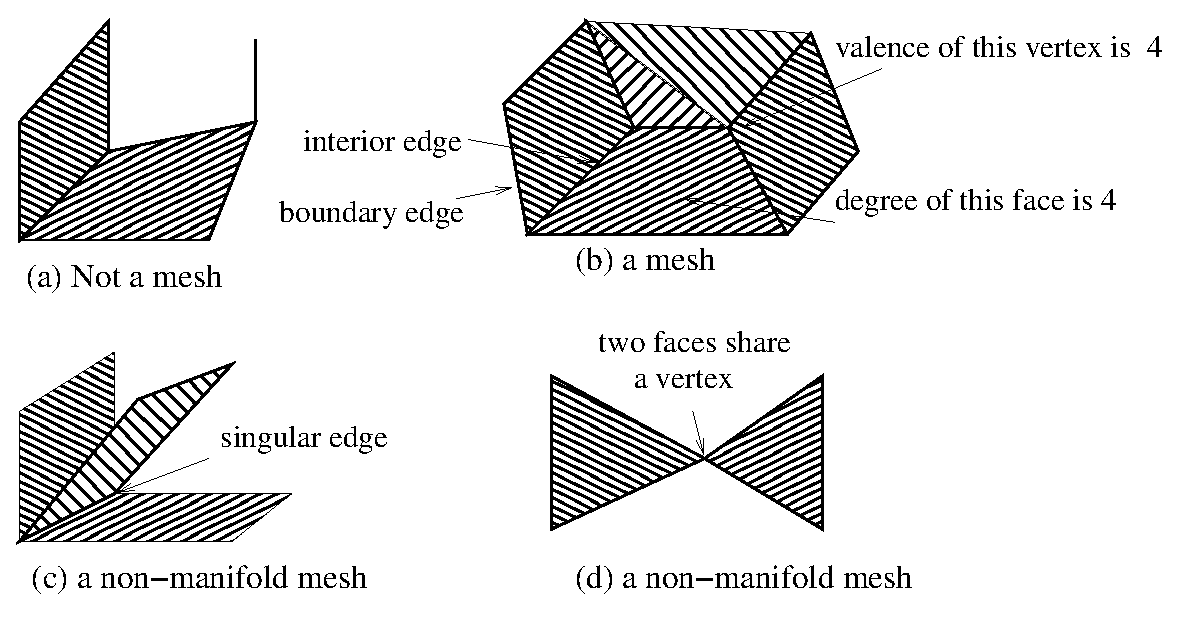
\includegraphics[width=0.8\textwidth]{figure2.1.eps}
\caption[Manifold mesh, non-manifold mesh and non-mesh]{ (a) is not
a mesh since one edge is incident to no face. (b) is a manifold
mesh. (c) is a non-manifold mesh since there is a singular edge.
(d) is a non-manifold mesh since two faces share only a
vertex.\label{mesh_non_mesh}}\
\end{figure}

    Polygonal meshes can be used as an approximation of the surfaces
    of 3D objects. In this case, some properties of the surface such
    as color and normal are often associated to the mesh. These
    properties can be categorized into two types: discrete attributes
    and scalar attributes \label{property}. Discrete attributes, such
    as material identifier, are usually associated to the faces, while
    scalar attributes, such as color, normal, and texture coordinate,
    are often associated to vertices or corners (the tuple (vertex,
    face)). The latter one is used because in the case of
    discontinuity, a vertex can have more than one scalar value. For
    example, if two smooth surface intersect at a curve, then vertices
    in this curve will have two different normal values. Therefore,
    the normal value should be associated to the tuple (vertex face).
    Then, polygonal meshes can be represented by $(K, V, D, S)$ where
    $D$ is the set of discrete attributes associated to face $f \in
    K$ and $S$ is the set of scalar attributes associated to corners $(v, f)$ in $S$.
    
    \subsection{Coding and Compression}
    A mesh is encoded first before it can be stored or
    transmitted. Coding is to represent a mesh with a sequence of
    digits. Compression is always combined with coding to save the storage space
    or the bandwidth needed in transmission. 
    There are two kinds of coding:
    single-rate coding and progressive coding. 
    Single-rate coded mesh can only be decoded when all data are available 
    whereas progressive coded mesh can be decoded with only part of data are available. 
    We will briefly introduce single-rate coding methods, and then concentrate on
    progressive coding methods, because the latter are more suitable for progressive streaming.
    
    \subsubsection{Single-rate Coding} \label{single_rate}
    In a mesh, three kind of information needs to be coded:
    connectivity, geometry and property. 
    Since most property data are associated to vertices, 
    in many compress algorithms they are treated as same as geometry data or even
    ignored. We introduce connectivity coding first, and then introduce geometry coding briefly.
    
    A triangle mesh is often represented as an array of vertex coordinates
    (geometry information) and an array of triangles (connectivity information). 
    A triangle is represented by the indices of its three vertices.
    In this representation, every vertex is indexed by all the
    triangles to which it is incident. Repeated references introduce
    redundancy. Therefore, triangle strip method is introduced to
    reduce this redundancy. In a triangle strip, a triangle fan, or a
    generalized triangle strip (a mixture of triangle strips and
    triangle fans) (see Figure \ref{strip}), 
    triangles can be represented with one index of vertex
    except the first triangle. 
    Deering \cite{218391} first introduced generalized triangular mesh, 
    which combining the generalized triangle strips with a vertex buffer,
    which is used to further reduce the bits used to represent indices. 
    Furthermore, Chow \cite{267103} introduced a method to
    decompose a mesh into triangle strips. 
    Bajaj, Pascucci and Zhuang \cite{789628} presented a coding method with layered
    decomposition. 
    Typically, a triangle layer is a generalized triangle strip. 
    \begin{figure}[ht]
    \centering
    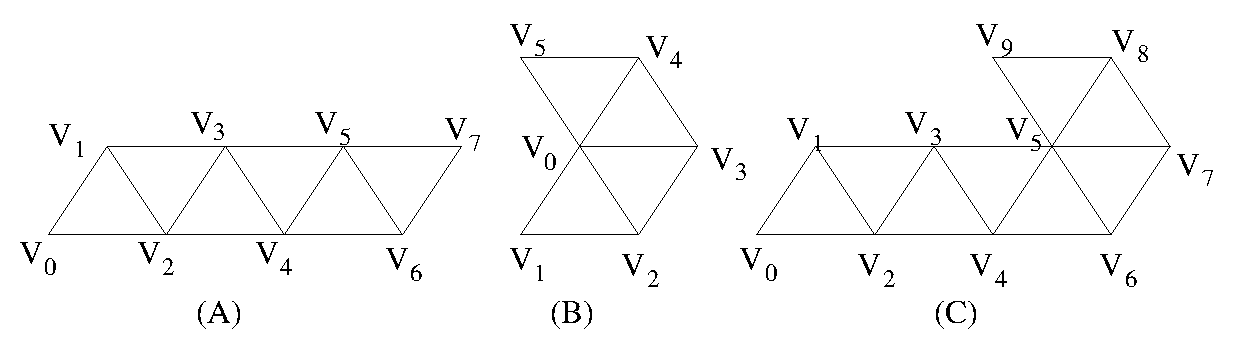
\includegraphics[width=0.6\textwidth]{strip.eps}
    \caption{(A)The triangle strip, (B)the triangle fan, and (C) the generated triangle strip.}\label{strip}
    \end{figure}

    Taubin and Rossignac \cite{274365} proposed a method named
    \emph{topological surgery}, which changes coding of a manifold
    mesh to coding of two trees: a vertex spanning tree and the dual of the triangles.
    Topological surgery has been implemented in MPEG-4 standard, and more details
    can be seen in the report of Taubin\cite{3d:Taubin}.
    
    Touma and Gotsman \cite{triangle:Touma} introduced a
    valence-driven approach to encode the connectivity by coding the
    valence of all the vertices in a specific traversing order. 
    The performance is further improved
    by Alliez and Desbrun \cite{alliez01valencedriven}, who also proved a
    upper-bound 3.24 bpv, exactly the theoretical value computed
    by Tutte \cite{census:Tutte} after enumerating all possible planar
    graphs.

    Several methods based on triangle conquest have also been
    proposed, such as \emph{cut-border machine} proposed by 
    Gumhold and Stra\ss{}er \cite{280836}.
    A significant advantage of this method is that it can be easily implemented
    in hardware and the decompression is very fast, which
    renders it to be very useful in real-time coding. 
    Another method named \emph{edgebreaker} is presented by Rossignac \cite{614421},
    and it is similar to the cut-border machine but has better
    compress efficiency and much slower decompression speed.
    
    After introduction of connectivity coding, we briefly introduce geometry
    coding. Most single-rate geometry compression methods involve three steps:
    quantization, prediction, and entropy coding.

    In VRML, geometry data is represented with 32 bit floating-point
    number, but this precision is highly beyond the perceiving
    capability of human eyes. Hence, quantization can be performed to
    compress the geometry data. Typically, each coordinate in a mesh is
    uniformly quantized to 8-16 bits integer.

    After quantization of vertex coordinates, prediction is taken in
    encoding by exploiting correlations between adjacent vertex
    coordinates. An effective prediction scheme generates prediction
    errors with highly compact distribution, which can be effectively
    encoded by entropy coders, such as Huffman coder or arithmetic
    coder. 

    More details about single-rate coding can be seen in the tutorial
    by Gotsman, Gumhold, and Kobbelt \cite{gotsman-simplification},
    the survey by Taubin \cite{3d:Taubin}, by Alliez and Gotsman
    \cite{recent:alliez}, and the survey by Peng, Kim and Kuo
    \cite{technologies:peng}.
    
    \subsubsection{Progressive Coding}
    Single-rate coded meshes can only be decoded after they are
    totally received, so they are not suitable for streaming. Therefore,
    some progressive coding schemes have been proposed. According to
    how the original mesh is simplified, these coding scheme can be
    categorized into three classes: progressive mesh based, vertex
    clustering based, and re-meshing based.
    
    \begin{description}
        \item[Vertex Clustering Based] 
            In vertex clustering based schemes, space is divided into cells
            following regular structure such as kd-tree \cite{566591} and 
            octree \cite{1073237}. All vertices inside a cell is represented
            by one delegate. Cells can be further divided into smaller cells
            and the quality of reconstructed model increases. Vertex clustering
            based coding can code geometry information efficiently, but it is 
            difficult to code connectivity information. Moreover, the quality
            of base mesh is poor.

        \item[Re-meshing Based]
            Re-meshing based method only keeps the shape of a model
            and does not keep the accurate topology. 
            A irregular mesh can be converted into a semi-regular mesh
            with similar shape. 
            %In a semi-regular
            %triangle mesh, the valence of most vertices is six, and therefore
            Because of the regularity of the new mesh,
            the connectivity information can be coded almost without cost.
            More details about these algorithms can be seen in the survey by Allienz and Gotsman
            \cite{recent:alliez}, the survey by Peng, Kim and Kuo
            \cite{technologies:peng} and the references therein.
            Besides losing the correct topology information,
            re-meshing based method usually code a mesh as a whole, 
            so there is no flexibility in streaming order.

        \item[Progressive Mesh Based]
            In this thesis, we concentrate on progressive meshes, which provide 
            the finest granularity in choosing streaming order and subset, 
            so we introduce the progressive mesh based coding in more details.
    \end{description}

    The progressive mesh (PM) \label{progressive_mesh}is first
    introduced by Hoppe in 1996 \cite{hoppe96progressive}. In this
    scheme, the simplification is based on \emph{edge collapse}, which
    collapses an edge into a vertex (see Figure \ref{split2}).
    After a series of edge collapse, a coarser \emph{base mesh} remains. 
    Then the PM is constructed by the base mesh and a series of \emph{vertex
    splits}, the inverse of edge collapse, in a reverse order.
    Rendering can be done in receiver side at any time after the base
    mesh is received. More vertex splits received, better
    approximation to the original mesh generated. After all
    the vertex split operations are received, the original mesh can be
    reconstructed without loss. \footnote{quantization error may exist
    when quantization is taken in geometry compression.}

    The base mesh can be encoded with the single-rate coding methods
    introduced in section \ref{single_rate}. Here, we introduce
    how to encode the vertex splits. 
\begin{figure}
\centering
\includegraphics[width=0.5\textwidth]{split2.eps}
\caption{Edge collapse and vertex split}\label{split2}
\end{figure}
    For connectivity
    information, we need to code $s$, $l$, and $r$, and for geometry
    information, we need to code the new position of $v_{s}$ and the
    position of $v_{r}$. If half collapse, which always collapse an
    edge to one of its ends (i.e. $v_{s}$ keeps unchanged), is used, 
    we only need to code the position of $v_r$. 
    
    If the number of vertices in current model is
    $V$, then $s$ can be any one of them, 
    and ${\lceil}log_{2}V{\rceil}$ bits are needed to encode $s$. 
    
    Many compression methods are proposed to reduce this cost.
    Hoppe \cite{efficient:hoppe} present an efficient implementation
    , in which the vertex splits is ordered such that next one
    is as close to current one as possible, and reduce the cost
    from $O(Vlog_{2}V$ to $O(V)$.
    In Karni, Bogomjakov, and Gotsman's paper \cite{602153}, 
    specific order of vertex split is also used to reduce the cost of connectivity. 
    The vertex sequence is generated by recursively cut a mesh to two
    balanced part with minimum cut. With their algorithm, the connectivity can
    be encoded with in average 4.5 bpv. 

    Another idea is to group many vertex splits together, 
    and efficiency will be improved at the cost of coarser granularity. 
    Taubin, Gu\'{e}ziec, Horn, and Lazarus \cite{280834} proposed the
    progressive forest split scheme (PFS), in which several edge
    collapse operations are combined together and the inverse operation splits a
    forest of edges and vertices. 
    Payarola and Rossignac \cite{614450}, 
    proposed compressed progressive mesh (CPM)\label{cpm} with similar
    idea. They group about $50\%$ vertex splits into one batch. To
    differentiate vertices to be split with others, one bit per vertex
    is used as indicative. 
    Some more methods have the similar idea
    but based on vertex removal (remove a vertex and triangulates the hole
    generated) \cite{319358}. 

    More methods exist to reduce the cost in encoding connectivity information.
    Some of them are extended from the single rate coding algorithms
    \cite{319426, 383281}. Some extend progressive mesh to directly
    encode non-manifold meshes \cite{258852}.

    All compression methods introduced above 
    have a common drawbacks. After compression, the 
    data become linear and they have to be decoded in a fix order. 
    Therefore, these methods improve the coding efficiency at the cost
    of losing flexibility, which is essential in streaming of high-resolution
    progressive meshes.
    
    Flexibility of choosing streaming order 
    is restricted by the dependency among the vertex splits.
    For a manifold mesh, a vertex split operation depends on the existence of
    \begin{itemize}
        \item 
    the vertex to be split ($V_s$ in Figure \ref{dstream:split}), 
        \item 
    two cut neighbors ($V_l, V_r$ in Figure \ref{dstream:split}). 
    \end{itemize}
    More dependencies exist if artificial folds are strictly forbidden \cite{258843, 258847}, 
    but in this thesis we ignore these dependencies since we can 
    tolerate temporary folds in our scheme.
     
    To et al. \cite{To1999} further remove the second dependency.
    In their method, if a cut neighbor does not exist during a vertex split,
    its ancestor will be used as the cut neighbor instead.
    Kim and Lee \cite{kim01truly} improve this method so that the final mesh
    can keep the original connectivity. 
    Kim et al. \cite{multiresolution:kim} propose a better scheme that enables
    an ordinary progressive mesh to be split in random order.

    These methods increase the flexibility, however, have a low coding efficiency.
    One solution proposed by Yang et al. \cite{progressive:Yang}
    is to divide the whole mesh into several segments and encode them
    separately to trade off between flexibility and compression efficiency.
    The weakness is that the size of the base mesh is relatively large
    since the original vertices in the border of segments are kept in the base
    mesh. Furthermore, the quality of the base mesh is uneven.

    Kim et al. \cite{multiresolution:kim}
    have proposed compression algorithms that allow random splitting of a mesh without
    sacrificing compression efficiency. This method is neat since it achieves comparable
    efficiency with other compression methods but keeps the largest flexibility.
    This algorithm, however. are not designed for 
	network transmission.  We extend it in this thesis and more details are introduced
    in Chapter \ref{c:rdstream}.  
    \subsection{3D streaming}
    \label{ss:intro:streaming}
    Given the backgrounds in modeling and coding, now we introduce some
    related works in 3D streaming. 
    The main concern in 3D streaming is how to improve the quality of the received
    mesh as fast as possible. Current studies can be categorized to three groups
    by how to achieve this objective.
    %Three main classes of work exist 
    %-- error resilient streaming, packetization, and view-dependent streaming.
    
    \subsubsection{Error Resilient Streaming}
    To improve the quality quickly, we need to mitigate distortion to the 
    rendered quality of rendered mesh in the presence of packet losses.

    At the transport layer, Al-Regib and Altunbasak \cite{3tpregib}, Li
    et al. \cite{Li2006}, and Chen et al. \cite{chen05hybrid} have
    investigated how to intelligently select either TCP or UDP for
    transmissions to trade off reliability and end-to-end delay.  Li et
    al. have also considered SCTP with partial reliability.
    Harris III and Kravets \cite{harris:design} propose a new
    transport protocol that exploits loss tolerance and
    partially-ordered property of 3D objects organized into trees of
    bounding volumes.

    At the application layer, the major error control techniques: error
    resilient coding, error protection, retransmission, and error
    concealment \cite{Park2003}, have all been applied to mesh streaming.  
    %Park et al.
    %\cite{error:Park} and Yan et al. \cite{error:Yan} focus on how to best
    %segment a progressive mesh into smaller partitions such that it is
    %more resilient to losses.  Al-Regib et al. \cite{1061349} consider a
    %joint-source channel coding method to determine appropriate level of
    %error protection to use.  Chen et al. \cite{chen05hybrid} also use
    %FEC for transmission of 3D data.  Error concealment is considered by
    %Park et al. \cite{Park2003}.  
    %Cheng et al. \cite{cheng07analytical}
    %argue for retransmissions as the main error control method, while
    %Tian \cite{Tian2006} uses selective retransmission in their system.
    
    Existing work in robust mesh compression aims to
    reduce dependencies among the mesh \cite{error:Park,error:Yan}.
    Similar to introducing key frames or restart marker in video/image
    coding, mesh segmentation is used to reduce the affected range of one
    packet loss. In robust mesh compression, a mesh is typically
    divided into several independent parts and then coded separately.
    Therefore the effect of one packet loss is confined to the part to which
    it belongs. The finer the partition is, the fewer the affected vertices
    are.  The coding efficiency, however, will decrease
    due to more redundancies and less correlation.

    Al-Regib and Altunbasak \cite{unequal:Al-Regib} proposed an
    unequal error protection method to improve the resilience of
    progressive 3D mesh based on CPM (compressed progressive meshes). 
    Forward error correction (FEC) codes are added to the
    base mesh and additional levels-of-detail information to maximize 
    the decoded mesh quality.  The method is similar to FEC protection 
    of video data.

    Chen et al. \cite{chen05hybrid} also applied FEC to streaming
    progressive meshes. They analyzed several transmission schemes:
    TCP only, UDP only, TCP with UDP, and UDP with FEC, and studied
    their effects experimentally on the transmission time and decoded
    mesh quality.
    
    Some studies use retransmission to recover the packet loss.
    For example, Tian \cite{Tian2006} uses selective retransmission in their system.
    We think retransmission is more suitable than FEC when the feedback
    channel is available, because there is no playback deadline in streaming
    of 3D meshes and data is always useful.

    Most of methods introduced above treat the meshes streamed as 
    traditional linear data. When the flexibiliy of progressive mesh
    is considered, a new questions arises: how to select a sending order
    to improve the quality quickly and mitigate the effect of packet loss.
    We call it \emph{packetization} problem.
    
    \subsubsection{Packetization}
    \label{ss:intro:packetization}
    Packetization of different model is tackled by
    Harris III and Karvets in \cite{harris:design}.   
    They proposed a protocol named On-Demand Graphic Transport Protocol (OGP)
    for transmitting 3D models represented as a tree of bounding volumes.
    A key component of the protocol is to decide which bounding volumes
    to send.  OGP begins with packing the largest possible subtree at
    the root and continues to pack the nodes in the subtree of
    acknowledged nodes in breadth-first order.  
    
    Gu and Ooi \cite{Gu:Packetization} were the first to look at
    the packetization problem for progressive meshes.  They model
    the packetization problem as a graph problem where the objective
    is to equally partition the graph into $k$ partitions with minimum
    cut size.  The problem is shown to be NP-complete and a heuristic
    is proposed.  They, however, assume that every vertex split contributes 
    to the rendered quality equally.
    
    In practice, the contribution of vertex splits can
    vary considerably. Therefore, when choose sending order, we
    need to trade off between minimize the dependency and sending 
    vertex split has higher contribution first. To achieve this objective,
    the effect of dependency needs to be quantitatively measured.
    Before us, however, there is no study is done for this problem.

    A commonly used metric of contribution of vertex splits is 
    Hausdorff distance between the original and reconstructed mesh \cite{cignoni98metro}.
    As Hausdorff distance is view independent, 
    bandwidth may be wasted in sending invisible vertex splits
    before the visible ones. Moreover, even among the visible vertex splits,
    the view-independent metric cannot reflect the real contribution to the visual quality of
    clients with different viewpoints. A vertex split that significantly
    changes a mesh may change the rendered image 
    only slightly.  A better metric for visual contribution of a vertex split,
    based on the rendered image on the screen, 
    needs to consider the receiver's viewpoint.
    Streaming of 3D models based on this metric is named \emph{view-dependent} streaming.

    \subsubsection{View-Dependent Streaming}
    The view-dependent approach first appeared as 
    a dynamic simplification method used for adaptive rendering of a complex 3D mesh
    \cite{258843, 258847}. Only vertex splits that contribute to the rendered
    image will be rendered, allowing real-time rendering of a complex mesh
    even with limited rendering capability.
    Besides progressive mesh, other multi-resolution representations, 
    such as vertex-clustering  and subdivision scheme,
    are used in view-dependent refinement systems \cite{245627, efficient:Alliez,602344}.

    Later, the view-dependent approach is used in progressive 
	streaming of 3D meshes.     
    In the scheme proposed by Southern et al. \cite{363375},  the client is stateless and
    maintains only the visible data. 
    To et al. \cite{To1999}
    and Kim et al. \cite{kim:view} proposed that received data are stored
    in the receiver even after they become invisible, 
    so they need not be resent when they are visible again. 
    In these papers, view-dependent approaches mainly aim at addressing
    limited rendering capability. 
    
    Yang et al. \cite{progressive:Yang} and
    Zheng et al. \cite{zheng:interactive}, on the other hand, use
    view-dependent streaming to address limited network bandwidth.
    Yang et al. proposed a scheme where the server chooses the appropriate resolution
    according to the available network bandwidth.
    Zheng et al. \cite{zheng:interactive} use prediction to
    reduce the effect of network latency and 
    compensate the round-trip delay with the rendering time.
     
    These systems use sender-driven approach and do not address
    server scalability issues. Due to the stateful design, 
    the sender-driven approach is difficult to be extended to
    support caching proxy and peer-to-peer techniques, two 
    common solutions to scalability. Before us, there is no study about
    how to implement a scalable 
    view-dependent streaming system without incurring high infrastructural cost.

    In a view-dependent steaming system, the streaming order of data highly
    depends on the interactivity of users. Designing a satisfying system
    requires a understanding of user behaviors in viewing 3D meshes.
    Most previous work on user interactions with 3D objects focused on design
    of specific interaction techniques (e.g., the study by Chen et al. \cite{chen88study}
    and Hinckley et al. \cite{hinckley97usability}). 
    As far as we know, there is no studies before us which study user behavior
    from the system design point of view.
    
    %\section{Problem Statement}
    %\label{s:intro:problem}
    %(summary)
    %\begin{itemize}
    %    \item No quantitative analysis has been done for 
    %        finding the effect of dependency 
    %        when progressive meshes are transmitted over lossy networks. 
    %    \item Sender-driven view-dependent streaming
    %        is not scalable to large number of receivers. 
    %    \item No peer-to-peer system 
    %        exists for view-dependent progressive mesh streaming. 
    %\end{itemize}
    \section{Objectives and Scope}
    \label{s:intro:objectives}
    To address the gaps mentioned in Section \ref{ss:intro:streaming},  
    %To address the problems introduced in Section 1.5, 
    the objectives of this thesis are listed as follows: 
    \begin{enumerate}
        \item The first objective of this thesis is
            to quantitatively analyze how sending order affects
            the rendered quality of progressive meshes 
            during transmission over lossy network. 
            To achieve this objective, 
            an analytical model is proposed
            to estimate the decoding time of
            each vertex split by considering both
            the mesh property and network condition. 
            This model could help us to find some insights
            about the effect of dependency. 
            In addition, it may be applied to find a better sending strategy, 
            and a greedy strategy is given in the thesis as an example. 
            Compared with methods based on simulation, 
            analytical model is more efficient and may be used
            in the real time so that the sending order
            can be adaptive to the network condition.
        \item The second objective is to implement view-dependent streaming
            in a more scalable way. A receiver-driven approach is proposed 
            to move the visibility decision from the sender to the receiver.
            The receiver-driven approach increase the scalability
            %not only because it reduce  overhead of the sender 
            %but also 
            because it makes the caching proxy and peer-to-peer much easier
            to be applied to remove the bandwidth bottleneck on the sender side.
            The application of receiver-driven approach could eventually
            make possible the view-dependent streaming of large meshes
            to huge number of receivers.
        \item
            The third objective of this thesis is to study user behavior from 
            the system design point of view, such as predictability (for prefetching)
            and locality of access patterns (for caching), similar to the spirit
            of the landmark studies for the Web \cite{huberman98web} and file system
            \cite {ousterhout85trace}. Moreover, we could generate random user 
            behaviors similar to real ones and use them in simulations, which 
            are useful in testing protocols and measuring system performance.
        \item 
            The last objective is to examine the possibility 
            of implementing a peer-to-peer view-dependent streaming system. 
            The receiver-driven approach proposed in this thesis 
            makes the peer-to-peer system possible, 
            but due to the flexibility of data, some new challenges exist,
            such as chunking and content discovery. 
            The prototype proposed in this thesis could give some insights
            to the future research on this area. 
            Eventually, peer-to-peer system should be an attractive way 
            to bring the streaming of large meshes into practice. 
    \end{enumerate}

    Only streaming of static 3D objects is considered in this thesis. 
    Streaming of 3D animations beyonds the scope of this thesis. 
    Moreover, streaming of 3D scenes is not concerned in this thesis.
    Instead, this thesis concentrates on streaming of one large mesh.
    Nonetheless, streaming of 3D scenes becomes easier when mature methods
    of streaming of single objects exist because a 3D scene is the collection
    of multiple single meshes. 
    Finally, this thesis focuses on the streaming of progressive meshes. 
    Streaming of other representations of 3D objects is not discussed in this thesis,
    but the methods proposed in this thesis should be possible
    extended to support streaming of other representations with some modifications.

    Following four chapters will introduce how we achieve our objectives in detail.
    Chapter \ref{c:model} introduces our analytical model and its applications, and
    Chapter \ref{c:rdstream} describes our receiver-driven view-dependent streaming
    protocol in detail. The result of our user study and its analysis is introduced
    in Chapter \ref{c:user} and topics about implementing P2P mesh streaming systems
    are discussed in Chapter \ref{c:p2p}. Finally, the whole thesis is concluded in
    Chapter \ref{c:conclusion}.
%\documentclass{acmsiggraph}
%\documentclass{acm_proc_article-sp}
\chapter{Analytical Model}
\label{c:model}
\def\tracea{UDP-High_result}
\def\traceb{UDP-Low_result}
\def\tracec{DCCP_result}
\def\mesha{Happy}
\def\meshb{Horse}
\def\meshc{Thai}
\def\mesh_h{Happy2}

\section{Introduction}
\label{s:model:intro}
    Advances in 3D scanning technology and mesh reconstruction
    algorithms have lowered the barrier in creating complex mesh
    objects and sharing them over the network.  For instance,
    software such as
    ZBrush is enabling easy creation of complex digital sculpture.
    The Stanford's Digital Michelangelo Project
    \cite{levoy00digital} digitized statues made by Michelangelo
    and provided a software, ScanView \cite{koller04protected},
    to allow users to remotely view the 3D version of the statues.
    Similar projects include the Digital Sculpture Project \cite{deroos2004dsp}
    and the project to digitize Rodin's sculptures \cite{miyazaki2006dab}. 
    Second Life, an online virtual world, is driven mostly by 
    user-created 3D objects, which are downloaded 
    on demand as users explore the virtual world.  
    These signs suggest that an increasing amount of
    3D mesh data will be available for remote viewing over
    the Internet.

    This paper targets at networked applications that require 3D meshes with high quality,
    such as virtual museum and virtual earth
    The amount of data constituting a high quality 3D mesh can be
    huge. For example, the statue of David, from the Digital
    Michelangelo Project, consists of 2 billion polygons.  After
    lossless compression, the total data size is 32 GB.  To reduce
    waiting time when downloading such a huge amount of data, a common
    technique for remote viewing is to encode a 3D mesh
    progressively \cite{lod}, allowing a low resolution version
    of the mesh to be transmitted and rendered with lower latency.
    The refinement information is continuously being transmitted,
    and the quality of the rendered model is incrementally improved
    over time.  Such progressive rendering is also useful in the
    case of virtual worlds such as Second Life. 
    In such applications, even though the models are typically smaller and simpler, 
    an arbitrary scene can contain numerous objects.
    Furthermore, such applications are interactive in nature.
    It is thus desirable for users to quickly visualize a coarse version
    of the scene first, instead of waiting for full objects to be
    downloaded before they can be displayed.
    %Note that our target applications are not 3D games, where strict high
    %interactivity is required and high quality 3D meshes are not commonly used.

    Progressive coding of meshes, much like progressive coding of
    video, introduces dependencies between data.
    Dependencies between data units can cause delay in decoding
    when sent over a lossy network -- a data unit
    cannot be decoded and displayed if one of the other data units
    it depends on is not received correctly. For example, in the
    context of video streaming, MPEG-encoded frames are inter-dependent:
        an I-frame has to be received and decoded properly
    before being able to decode the subsequent P-frames and B-frames
        referencing this I-frame (either directly or indirectly).  Another
    example is in layered coded video, where the base layer has
    to be received before the enhancement layers can be decoded.
    The effects of dependencies in the context of video streaming
    have been well studied in the literature \cite{boyce98}.   Multi-resolution 3D
    objects also have dependencies between different level of details.
        For progressive meshes, the mesh is refined by successive
    \textit{vertex splits} (see Figure~\ref{model:split}).  Thus,
    dependencies exist between the original vertex and its one
    ring (the direct neighbors of the vertex)
    and the vertices and triangles created by the vertex split.
    The effects of these dependencies on decoded mesh quality, however,
    are not well understood.  Due to the fundamentally different
    nature of progressive mesh and video data, what we learn from
    video streaming research does not apply.  This paper aims to study
    the effect of dependencies in progressive mesh streaming by
    proposing an analytical model, relating the decoded mesh quality
    of progressive mesh to packet loss rate, given the dependencies
    among vertex splits.

    The decoded mesh quality at a given time $t$ is determined by 
    the vertex splits that are decoded before $t$ and their contribution to the overall mesh quality.
    To estimate the decoded mesh quality at time $t$, our analytical model
    predicts the decoding time of each vertex split.  The total contribution of vertex
    splits decodable before $t$ gives the quality.  To predict the decoding time, we first
    express the expected time for receiving each packet
        in terms of loss rate, round trip time, and sending rate.
    A received vertex split has to wait for the vertex splits
    it depends on to arrive before it can be decoded.
    Therefore the received time of a vertex split is not always equal to its decoding
    time.  Our model gives an expression for the expected
    decoding time given the dependencies among the vertex splits.
    Furthermore, we propose
    a metric to measure the contribution of 
    vertex splits to the
    decoded mesh quality. The decoded mesh quality then can be computed 
    after we know the expected decoding time of every vertex split
    and its contribution.

    Our analytical model is useful in several ways.  First,
    we can analytically evaluate different strategies for streaming
    a progressive mesh.  For instance, packetization of vertex
    splits affects the intermediate decoded mesh quality
    at the receiver.  Evaluating different packetization scheme
    using simulation is an option, but
    it may take many experiments to obtain accurate
    expected values.  Our model computes the expected value easily.
    Second, our model can also help in developing a better sending
    strategy.  The quality of the decoded mesh depends on
    various factors, which include not only network conditions such
    as loss rate and round trip time, but also the order, the
    dependency, and the importance of the data.
    The last three factors are in turn affected by the packetization
    strategy.  Our model can estimate the effect of each factor on the
    decoded mesh quality.
    As such, we can make the right trade-off between these factors
    during transmission to improve the quality.
    Finally, we derive closed-form expressions in two extreme cases,
    giving us insights into the importance of dependencies on the
    decoded mesh quality.

    %Now we clarify the scope of this paper.
    %First, although some other representations
    %of 3D objects exist, such as pointed based representations, we concentrate on 3D meshes. 
    %We are not saying 
    %mesh is the only or the best representation, but it is the most popular one.
    %Moreover, progressive mesh supports finer granularity of progressivity compared with progressive pointed based methods.
    %Nonetheless, our model actually can be applied to any partially ordered data. 
    %For example, we successfully applied it on streaming of digitized plants \cite{plant:seb}
    %Second, in our implementation, only manifold meshes are supported. Most Statues could be represented 
    %as manifold-meshes, and every non-manifold meshes could be transformed to manifold meshes.
    %Third, we only consider static meshes in this paper, and to support the animation is an interesting 
    %future research topic.  
    %(Geraldine)Let us now clarify the scope of our paper. 
    %First, the analysis and strategy we proposed to apply to any partially ordered data 
%    (Multi-resolution 3D models are indeed partially ordered chunks), 
%    e.g. pointed based model organized as QSplat tree. 
%    Here we concentrate on progressive 3D meshes. 
%    Meshes are not necessarily the best representation, 
%    but they are the most popular one. 
%    Moreover, progressive mesh supports finer granularity of progressivity 
%    than other multi-resolution representations. 
%    Nonetheless, our model has actually being applied to other partially ordered data, 
%    digitized plants \cite{plant:seb}.

    Our analytical model is general and can be applied to any 
    partially-ordered data without playback deadline.  We
    choose to concentrate on progressive 3D meshes (which are indeed 
    partially ordered chunks) in this paper. 
    While meshes are not necessarily the best 3D representations, they 
    are popular and support finer granularity of progressivity 
    than other multi-resolution representations. 
    Other examples of such partially-ordered data include point-based models 
    organized as QSplat trees \cite{rusinkiewicz:qsplat} and digitized plants.  
    We have actually applied our analytical model to the latter \cite{plant:seb}.
    
    A preliminary version of this analytical model was previously published 
    \cite{cheng07analytical}.  In this journal version, we extended our work
    with detailed proofs and analysis, as well as extensive validation of our 
    model under a variety of network conditions using different progressive mesh models.

    The rest of the paper consists of six sections. Section~\ref{s:model:bg} provides the background on this paper.
    We describe progressive mesh and how it
    introduces dependencies (Section~\ref{s:model:mesh})
    and present related work in the area
    of 3D objects streaming (Section~\ref{s:model:related}).
    %Section~\ref{s:metric} introduces our evaluation metric
    %for intermediate decoded mesh quality.
    Section~\ref{s:model:model} introduces our analytical model.
    We then describe the applications of our model.
    In Section~\ref{s:model:effect}, we study two hypothetical extreme
    cases, and show the effect of dependencies on
    decoded mesh quality.
    In Section~\ref{s:model:quality}, we show how our
    model can be used to analytically compute the expected
    decoded mesh quality and how this expected quality
    %Section~\ref{s:expected_quality}
    %shows how our model can be used in computing the expected
    %rendering quality given the dependencies and packet loss
    %probability.
    can be used to design a packetization strategy for transmitting
    progressive mesh.  Section~\ref{s:model:experiment} presents validation
    of our model and evaluation of the proposed packetization strategy,
    using network traces using UDP and DCCP under various
    network conditions.  
    Section~\ref{s:model:conclude} concludes by
    reflecting on the insights we gain from our model and its
    implications.

\section{Background and Related Work}
\label{s:model:bg}
\subsection{Progressive Mesh}
\label{s:model:mesh}

    Progressive transmission and rendering of 3D objects
    requires multi-resolution representations of data. One such 
    representation, progressive mesh, is proposed by Hoppe
    \cite{hoppe96progressive}.
    The technique is based on an
    operation called \textit{edge collapse}, and its reverse
    operation, \textit{vertex split}.  Given a (non-progressive)
    3D mesh, the technique applies a series of edge collapses,
    simplifying the model by reducing the number of vertices and
    faces.  The final, simplified model obtained after this
    process becomes the \textit{base model}.  Given a base model,
    we can reconstruct the original model by reversing
    the edge collapse operations through \textit{vertex splits},
    incrementally adding new vertices and faces. So, a
    progressive mesh can be represented by the base
    model and a series of vertex splits.  There are
    dependencies between vertex splits and the base model, as well as
    among the vertex splits.  A vertex split
    operation might need a vertex or a face created by another
    vertex split as input.  Figure~\ref{model:split} illustrates edge
    collapse and vertex split operations.

    \begin{figure}
    \begin{minipage}[b]{0.5\linewidth}
    \centering
    \epsfig{file = figures/split2.eps, height = 0.9in}
    \caption{Edge collapse and its reverse vertex split\label{model:split}}
    \end{minipage}
    \hspace{0.2cm}
    \begin{minipage}[b]{0.5\linewidth}
    \centering
    \epsfig{file = figures/dag1.eps, height = 1.2in}
    \caption{Dependency between vertex splits represented as a DAG.\label{model:dag2}}
    \end{minipage}
    \end{figure}

    %% Here we added the paragraph to justify the choice of the model
  Progressive meshes are well adapted for streaming since
  they offer the finest level of progressivity --
  it allows refinement at the granularity of vertices. 
  This progressivity is crucial for our
  application since a streamed vertex split only depends on
  the vertex splits that generated its neighbors, and not on other
  refinement operations of the same level (like for
  subdivision surfaces). Therefore, only dependencies among
  the vertex splits are crucial.

    Many extensions and variations to Hoppe's
    progressive mesh have been proposed (e.g.,
    \cite{614450,319358,383281,multiresolution:chen}).  The main idea
    behind these extensions is to combine multiple
    operations into one, thereby further reducing the
    redundancy and improving the efficiency. In particular, Pajarola and 
    Rossignac proposed a compressed progressive mesh (CPM) representation to reduce
    the size of a progressive mesh \cite{614450}. While this paper
    only considers the original progressive mesh, our
    model is general enough to model many of these
    extensions. 

    Significant differences exist between progressive mesh
    streaming and video streaming.  First, in video streaming,
    every packet should be received in time, or it will not
    be played back.  Hence, generally sending new data is more
    important than re-sending old data. On the contrary,
    in streaming of a progressive mesh, old data is
    usually more important than new one, since the
    reconstruction begins with the most significant refinement.
    Given this observation, retransmission of a lost packet is
    not only useful, but it should also take priority
    over transmission of new packets.

    Second, in progressive mesh, there is no strict order
    of vertex splits rendering order, unlike in video where
    frames must be displayed in sequence. A received vertex split
    can be rendered immediately as long as all the vertex splits
    it depends on have been received.  When a packet is lost, the
    subsequent received packets may still be decodable.  Those
    vertex splits received afterwards that depend on the
    lost packet, however, have to wait until the lost packet
    is retransmitted successfully before they can be displayed.
    This observation hinted that we should reduce the dependencies
    between packets as much as possible, since dependencies cause
    delay in rendering details generated by vertex splits.

    Third, a video frame is usually larger than a packet,
    causing the streaming application to split the video frame
    into several packets.  On the other hand, in progressive mesh,
    a vertex split is small (in the order of 10 - 15 bytes).  Thus,
    before the application transmits the mesh, it needs to group
    vertex splits into packets.   This \textit{packetization}
    process affects the dependencies among the packets, which in
    turn affects the delay in rendering if some packets are lost.
\\
\subsection{Related Work}
\label{s:model:related}

    Given the background in progressive mesh, we now describe
    related research in network transmissions of progressive mesh. 
    Three main classes of work exist 
    -- error resilient compression, error control, and
    packetization.

    Existing work in robust mesh compression aims to
    reduce dependencies among the mesh \cite{error:Park,error:Yan}.
    Similar to introducing key frames or restart marker in video/image
    coding, mesh
    segmentation is used to reduce the affected range of one
    packet loss. In robust mesh compression, a mesh is typically
    divided into several independent parts and then coded separately.
    Therefore the effect of one packet loss is confined to the part to which
    it belongs. The finer the partition is, the fewer the affected vertices
    are.  The coding efficiency, however, will decrease
    due to more redundancies and less correlation.

    Al-Regib and Altunbasak \cite{unequal:Al-Regib} proposed an
    unequal error protection method to improve the resilience of
    progressive 3D mesh based on CPM (compressed progressive meshes). Forward error
    correction (FEC) codes are added to the
    base mesh and additional levels-of-detail information to maximize 
    the decoded mesh quality.  The method is similar to FEC protection 
    of video data.
    As argued in the previous section, we believe that for streaming
    of 3D meshes, retransmission is always a better choice (except in
    cases such as multicast where retransmission is not scalable).
    Chen et al. \cite{chen05hybrid} also applied FEC to streaming
    progressive meshes. They analyzed several transmission schemes:
    TCP only, UDP only, TCP with UDP, and UDP with FEC, and studied
    their effects experimentally on the transmission time and decoded
    mesh quality.
    Al-Regib et al. proposed an application layer protocol, 3TP,
    for streaming of 3D models \cite{3tpregib}, combining both TCP 
    and UDP.  In 3TP, important packets are sent using
    TCP, while the rest are sent with UDP to minimize delay.

    
    Packetization of different model is tackled by
    Harris III and Karvets in \cite{harris:design}.   They proposed
    a protocol named On-Demand Graphic Transport Protocol (OGP)
    for transmitting 3D models represented as a tree of bounding volumes.
    A key component of the protocol is to decide which bounding volumes
    to send.  OGP begins with packing the largest possible subtree at
    the root and continues to pack the nodes in the subtree of
    acknowledged nodes in breadth-first order.  
    Gu and Ooi \cite{Gu:Packetization} were the first to look at
    the packetization problem for progressive meshes.  They model
    the packetization problem as a graph problem where the objective
    is to equally partition the graph into $k$ partitions with minimum
    cut size.  The problem is shown to be NP-complete and a heuristic
    is proposed.  They, however, assume that every vertex split is
    equally important.  In practice, the importance of vertex splits can
    vary considerably.  

    These existing studies are mainly concerned with dependencies
    (packetization and mesh segmentation) and importance
    of mesh data (unequal error protection and use of reliable protocol), 
    two factors that affect the quality of decoded meshes.  None, however,
    have looked at both factors and characterize 
    their effect on quality.  We aim at achieving this by proposing
    an analytical model.

\section{Analytical Model}
\label{s:model:model}
    We now develop an analytical model for transmission of
    progressive mesh over lossy networks.  We first need to model
    the progressive mesh and the network.  Since typically
    the base model is small (less than 1\% of the total size) 
    and is transmitted using reliable
    transport protocols \cite{3tpregib}, we assume that the
    base model has been received by the
    receiver. We will focus on modeling the vertex splits,
    which can be represented as a directed acyclic graph (DAG)
    (see Figure~\ref{model:dag2}). In the DAG, nodes represent
    the vertex split operations, and edges represent the dependency
    between these operations. We assign each node a weight,
    which corresponds to the importance of the vertex split.
    We will use the terms node and vertex split interchangeably
    in this paper.

    On the sender, vertex splits are grouped into packets,
    each containing equal number of vertex splits.  We say packet $P$ is a \textit{parent packet}
    of the vertex split $v$ if %the vertex split 
    $v$ 
    depends on at least one vertex split in $P$.  Therefore, a vertex split
    can be decoded only after the packet containing it and all its
    parent packets are received.

\if0
\begin{figure}
\centering
\epsfig{file = figures/dag1.eps, height = 1.2in}
\caption{Dependency between vertex splits represented as a DAG.\label{model:dag2}}
\end{figure}
\fi

    Let $B$ be the average
    sending rate\footnote{decided either by the available bandwidth or by TCP friendly requirement} and $p$ be the packet loss rate.
    In the model, we assume that packet losses are independent to each other for simplicity.
    In Section \ref{s:model:experiment}, we %will
    show that our model still works well under realistic packet losses (more bursty).
    We assume a retransmission-based protocol -- the sender resends a packet when its loss is detected.
    %a retransmission request (NACK) is sent back to the sender,
    %triggering a retransmission.  
    %the sender resends this packet. 
    Let $T_d$ be the
    average period between the time a packet %$P$ 
    is sent and the
    time %$P$'s 
    its loss is detected at the sender.
    %$T_d$ is the round trip time plus some constant.
    While $B$, $p$, and $T_d$ are likely to varies in practice during to network dynamics, 
    we adopt a common technique in performance modeling by constructing our model using 
    their average values and assuming that they are constants.
    We study the effects of this assumption in Section \ref{s:model:experiment}.

    We discretize time into slots.  Each slot is the time to
    send one packet.  Thus, one time unit is $L/B$ seconds, where $L$ is the
    packet size.  
    The time $T_d$ is normalized to this
    time unit.  Thus, $T_d$ can also be interpreted as the number
    of packets transmitted between sending a packet $P$ and detecting
    the loss of $P$.  Moreover, at the sender,
    we define the time the first packet is sent as time $0$, whereas, at
    the receiver, we define the time the first packet is received (if it
    is not lost) as $0$.  Therefore, a packet sent at time $t$ will be 
    received at time $t$ if it is not lost.  Thanks to the different 
    timeline at the
    receiver, we avoid an additional term, $RTT/2$, in
    equations related to the received time and decoded time. 
    We denote the $i$-th packet sent (and not retransmitted) as $P_i$, where $i = 0, 1, ...$.
    Table~\ref{t:model:notation} summarizes these notations as well as
    other major notations used in this paper.

% NOTATION

    \begin{table}
    \begin{centering}
    \begin{tabular}{|r|l|}
    \hline
    $L$ & packet size \\
    $B$ & sending rate \\
    $p$ & packet loss rate \\
    $T_d$ & time between sending a packet and \\
          & receiving its NACK\\
    $S_i$ & sending time of $P_i$ (wrt. sender time)\\
    $R_i$ & received time of $P_i$ (wrt. receiver time)\\
    $D_j$ & the time vertex split $j$ is decoded at the receiver \\
    $w_j$ & the importance of vertex split $j$ \\
    $N_{d,t}$ & number of packets decoded at time $t$ \\
    $N_{r,t}$ & number of packets received at time $t$ \\
    $\Delta_t$ & increase in expected number of decodable packet at time $t$\\
    \hline
    \end{tabular}
    \caption{Notations used in our model\label{t:model:notation}.}
    \end{centering}
    \end{table}

    With that background, we are able to explain how we obtain the
    expected value of sending time, received time, and decoding time
    of a vertex split.
\if\showproof0
    Due to space constraints, we will only sketch the proofs in this
    paper.
\fi

\subsection{Sending Time and Receiving Time}
%\newtheoremstyle{definition}
Let $S_i$ be the time when $P_i$ is sent. %If $k$ packets have been lost and retransmitted before $S_i$ then packet $i$ is sent at time $S_i=i+k$. Lemma~\ref{theorem_ts} computes the probability of this event and the expected value $E[S_i]$ of the time when the packet $i$ is sent.
Lemma~\ref{model:theorem_ts} computes the distribution of $S_i$ and the expected value $E[S_i]$.
\begin{lemma} \label{model:theorem_ts}
If $i \geq T_{d}$, %then for any $k \geq 0$,
\begin{eqnarray*}
E[S_i]          &=& (i - T_d + 1)\frac{1}{1-p} + T_d - 1.
%$E[S_i]          = (i - T_d + 1)\frac{1}{1-p} + T_d - 1$.
\end{eqnarray*}
%Pr(S_i = i+k)     &=& \binom{i-T_d+k}{k}p^k(1-p)^{i-T_d+1}\\
%ooiwt - no need pdf in the lemma since not using it elsewhere.
Otherwise, %if $i < T_d$, then 
$S_i = i$.
\end{lemma}
\if\showproof1
\begin{proof}
    If $i<T_d$, then $S_i = i$ since no retransmission exists.
    Now we consider the case when $i \geq T_d$.
    The number of transmissions before one successful transmission
    is a random variable with geometric distribution and its
    expected value is $1/(1-p)$.  Therefore, the expected value of
    total transmissions after time $T_d$ when there are
    $i - T_d + 1$ known successful transmissions is $(i - T_d +1)/(1-p)$.
    Hence, we have 
    %\begin{displaymath}
        $E[S_i]          = (i - T_d + 1)\frac{1}{1-p} + T_d - 1$.
    %\end{displaymath}
    %Between time $0$ and time $i+k$ there are $i+k+1$ time slots.
    %Among them, $i+1$ slots are used to send new packets (packet $0$
    %to packet $i$) and $k$ slots are used for retransmissions.
    %Retransmissions cannot happen before time slot $T_d$ because the earliest
    %time to detect a packet loss is $T_d$. Moreover, time slot
    %$i+k$ is used to send the new packet $i$. Hence, the $k$ retransmissions
    %only happen in $i+k-T_d$ time slots 
    %(from time slot $T_d$ to time slot $i+k-1$), so there are in total
    %$\binom{i-T_d-k}{k}$ possible situations. 
    %
    %Since packet $i$ is sent at time $i+k$, $i+1$ slots are used for
    %sending new packets and $k$ are used for retransmissions.
    %Retransmissions cannot happen at the first $T_{d}$ slots (no packet
    %loss can be detected before time $T_d$), and the time slot $i+k$ is
    %used for transmission of new packet $i$. 
    %Therefore, the $k$ retransmissions can only happen between $T_d$ and
    %$i+k-1$, in total $i-Td+k$ slots. 
    %Moreover, 
    % 
    %%Time slot $t$ is used for retransmission if and only if the packet sent
    %%at time $t-T_d$ is lost, so the probability for a time slot to be used
    %%for retransmission is also $p$. From $T_d$ to $i+k$, $k$ time slots
    %%are used for retransmissions and $i-T_d+1$ time slots are used to send
    %%new packets. Therefore, for each possible situation,
    %%the probability is $p^{k}(1-p)^{i-T_d+1}$.
    % 
    %A retransmission corresponds to a packet loss happens $T_d$ before,
    %so a slot. 
    %Therefore, among the $i+k-T_d+1$ time slots from $T_d$ to $i+k$, 
    %a time slot is used for retransmission in probability $p$ and 
    %sending new packet in probability $1-p$. 
    %Since the time slot $i+k$
    %is used to send packet $i$, so the $k$ retransmissions can only
    %happen in the rest $i-T_d+k$ time slots.
    %
    %%Hence, we have
    %%\begin{displaymath}
    %%Pr(S_i = i+k)     = \binom{i-T_d+k}{k}p^k(1-p)^{i-T_d+1}.
    %%\end{displaymath}
    %
    %%The number of transmissions before one successful transmission
    %%is a random variable with geometric distribution and its
    %%expected value is $1/(1-p)$.  Therefore, the expected value of
    %%total transmissions after time $T_d$ when there are
    %%$i - T_d + 1$ known successful transmissions is $(i - T_d +1)/(1-p)$.
    %%Hence, we have 
    %%\begin{displaymath}
    %%    E[S_i]          = (i - T_d + 1)\frac{1}{1-p} + T_d - 1.
    %%\end{displaymath}
    \end{proof}
\else
    % Proof sketch
    %\textbf{Proof sketch}
    
    \begin{proof}
    Whether a packet is sent successfully or not can be known only after $T_{d}$.  
    At time $i + k$ ($k \geq 0$),  the result of first $i + k - T_d + 1$ transmissions are
    known (we call them \textit{known transmissions}), but the result of the following $T_d - 1$
    transmission remains unknown (we call it \textit{unknown transmission}).  For $t \geq T_d$,
    a new packet is sent at $t$ only when the
    transmission at $t-T_d$ is known to be successful.  Hence, if packet $i$ is sent at
    $i+k$, then among the $i + k - T_d + 1$ known transmissions, $i - T_d + 1$
    transmissions are successful and $k$ transmissions fail.
    The variable $k$ has a negative binomial distribution,
    and the expression for $Pr(S_i = i+k)$ follows.
    \end{proof}

    The total number of transmissions until a packet is successfully sent is
    a random variable following geometric distribution with expected value of
    $1/(1-p)$. Therefore, the expected value of total transmission number
    until $i - T_d + 1$ packets are successfully sent is $(i-T_d+1)/(1-p)$.
    Including the subsequent $T_d - 1$ unknown transmissions, we have the expression
    for $E[S_i]$.  \QED
\fi

    
Let $R_i$ denote the time a packet $i$ is received.
The probability that a packet $i$ is received at time $t$
is given as follows.
\begin{lemma}
\label{l:model:preqt}
  \begin{equation*}
    Pr(R_i = t) = \left\{
   \begin{array}{ll}
    (1-p)p^{n_{i,t}} & \mbox{if } (t-S_i) \mod T_d = 0  \\
        0                & \mbox{otherwise}
   \end{array}
   \right.
\end{equation*}
    where $n_{i,t}=\lfloor(t - S_i)/T_d\rfloor$ is the number of times packet $i$ was lost when $R_i = t$.
\end{lemma}

    %\textbf{Proof sketch}
    \begin{proof}
    The lemma follows from the fact that a packet can only be
    received at a time that is a multiple of $T_d$ after the
    first time it was sent. %\QED
    \end{proof}

    Note that here $S_i$ is a random variable but we approximate
    the decoding time by using the expected value of $S_i$ computed
    from Lemma~\ref{model:theorem_ts}.  This approximation is accurate
    enough (as shown in the next subsection) as long as the variance
    of $S_i$ is small.
    %\footnote{This approximation
    %leads to the possibility of two packets arriving at exactly
    %the same time.  In this case, we break ties by randomly reordering
    %the arrival of the packets}.

\begin{lemma}
\label{l:model:prlet}
\begin{equation*}
Pr(R_i \leq t) = 1 - p^{n_{i,t}+1}.
%$Pr(R_i \leq t) = 1 - p^{n_{i,t}+1}$.
\end{equation*}
\end{lemma}

    %\textit{Proof sketch}
    \begin{proof}
    A packet is received strictly after time $t$ if and only if the packet
    is lost at least $n_{i,t}+1$ times and the probability is
    $p^{n_{i,t}+1}$. 
    %Given $t$, the probability that a packet is received strictly after
    %time $t$ is the same as the probability that the packet has been
    %lost $n_{i,t} + 1$ times, or $p^{n_{i,t}+1}$.  
    Lemma~\ref{l:model:prlet} follows. %\QED
    \end{proof}

\subsection{Decoding Time of a Vertex Split}

    Once we expressed both sending time and receiving time,
    we can approximate the decoding time of a vertex split $v$, denoted
    as $D_v$.

    Let $\mathcal{P}(v)$ be the set of
    all parent packets of the vertex split $v$ and the packet including $v$, then the
    probability that vertex split $v$ can be decoded at time $t$
    is given by the probability that one of the packet in $\mathcal{P}(v)$
    is received at time $t$ and all other packets in $\mathcal{P}(v)$
    is received before time $t$.
    \begin{eqnarray}
    \label{e:model:pdvt}
        Pr(D_v = t) = \sum_{i \in \mathcal{P}(v)} \frac{Pr(R_i = t)}{Pr(R_i < t)} \prod_{k \in \mathcal{P}(v)} Pr(R_k < t).
    \end{eqnarray}

    Lemma~\ref{l:model:preqt} and \ref{l:model:prlet} give the expression
    for $Pr(R_i=t)$ and $Pr(R_i<t)$ respectively.
    Once we have the probability distribution of $D_v$, we can
    estimate the expected decoding time of a vertex split $v$
    with
    \begin{equation}
    \label{e:model:e_et}
        E[D_v] = \sum_{j=t}^{\infty}jPr(D_v = j).
    \end{equation}

    Since the probability $Pr(D_v = t)$ decreases exponentially
    as $t$ increases, in practice we can numerically estimate the
    expected decoding time by considering only the first few
    terms of the sum.  In this paper, we consider $j$ from $S_i$ to $S_i + 3T_d$,
    which we found to be accurate enough for practical purposes.
    That is,
    a packet is considered to be lost at most three times in a row.
    For larger loss rate, one can consider more terms to trade-off
    computation time and accuracy.


    Our analytical model is useful in several ways.  
    These equations can help us in understanding the effect of dependency (see Section \ref{s:model:effect}) when transmitting 
    a progressive mesh over a lossy network.  Our model can lead to some simple close form equations in two special cases.  
    We can also compute the expected decoded quality analytically, leading to a faster alternative to 
    simulation (see Section \ref{s:model:analytical_quality}) as a way to evaluate the effects of network conditions on
    progressive mesh streaming.
    Moreover, a better packetization algorithm can be designed based on this analytical model (Section \ref{s:model:scheduling}). 
    We introduce these applications of our model next.


\section{Effects of Dependencies}
\label{s:model:effect}

    This section discusses the effects of dependencies
    on the number of decodable packets, as a function of
    $p$ and $T_d$.  As mentioned in Section~\ref{s:model:mesh},
    packetization at the sender may affect
    decoded mesh quality.  We quantify 
    this effect by estimating the number of
    decodable packets at a given time for two extreme cases
    of dependencies.  The effects of any other dependency
    will be bounded by what we obtained for these two extreme cases.

    In the first case (ideal
    case), there is no dependency among packets.
    In the second case (worst case), a packet depends on all other packets
    sent previously.  Note that these two dependency models are
    independent of any packetization scheme.
    Moreover, we are computing the number of decodable \textit{packets} rather
    than \textit{vertex splits}.  This simplification does not affect
    the accuracy of our model
    since in the ideal case, we can assume that all vertex splits
    in a packet are decodable as soon as the packet is received (no dependencies
    among packets).  In the worst case, if a packet's dependency is not
    satisfied, then all vertex splits contained in that packet are
    not decodable.  Thus, the number of decodable packets is
    proportional to the number of decodable vertex splits in these two extreme
    cases.

    Let $N_{r,t}$ be the number of received packets at time $t$ and
    $N_{d,t}$ be the number of decoded packets at time $t$.   We show
    how to compute the expected value of $N_{d,t}$ for the two
    extreme cases in the next two subsections.

\subsection{Ideal Case}
\begin{theorem}
\label{t:model:ideal}
    In the case with no dependencies among the packets,
    \begin{eqnarray*}
%    Pr(N_{r,t} = k) &=& \binom{t+1}{k}p^k(1-p)^{t+1-k},\\
    E[N_{r,t}] &=& E[N_{d,t}] = (t+1)(1-p).
    \end{eqnarray*}
\end{theorem}
    %\textbf{Proof Sketch}
    \begin{proof}
    In the ideal case, each packet can be decoded independently
    regardless of other packets.  Thus, at any time $t$,
    $N_{d,t} = N_{r,t}$.
    Let $a_i$ represents the result of a transmission at time $i$,  
    that is
    \begin{displaymath}
    a_i = \left\{\begin{array}{ll}
    1 & \textrm{if transmission is successful}\\
    0 & \textrm{if transmission is failed}\\
    \end{array}\right.
    \end{displaymath}
    The expected number of successful transmissions at time $t$ is
    \begin{eqnarray*}
    E\big[\sum_{i=0}{t}a_i\big] = \sum_{i=0}{t}E[a_i] = \sum_{i=0}{t}(1-p) = (t+1)(1-p)
    \end{eqnarray*}
    %The number of successful transmission at time $t$ is equivalent to
    %the number of successful Bernoulli trials out of $t+1$
    %transmission\footnote{recall that the first transmission is at time 0}.
    %Theorem~\ref{t:ideal} follows.
    %\QED
    \end{proof}

\subsection{Worst Case}

    

    In the worst case, a packet depends on all previous packets (packets
    with smaller index).  The expected number of packets decodable at
    time $t$, is given by the following equation:
    \begin{eqnarray}
    \label{e:model:endt}
    E[N_{d,t}] = \sum_{i=0}^{m} \prod_{j=0}^i Pr(R_j \le t),
    \end{eqnarray}
    where $m$ is the total number of packets\footnote{When $p=0$, $N_{d,t}$ is always $t+1$.  We assume non-zero $p$ in this section.}.

    Obtaining a close form formula for $E[N_{d,t}]$ is more tricky.
    
    We therefore first derive a close form formula for $\Delta_t$, which is 
    the increase of the expected number of packets decodable at time $t$,
    that is, $\Delta_t = E[N_{d,t}] - E[N_{d,t-1}]$. 
    We let $\Delta_0$ be $(1-p)$ since
    the expected number of packets decodable at time 0 is $(1-p)$.

    Suppose $P_0$ is successfully received at time $0$.  We remove $P_0$
    from the dependency graph, reducing the dependency graph to a 
    graph with the same dependency structure
    but with one less packet.  The expected number of decodable
    packets from time $1$ to time $t$ is the same as the expected
    number of decodable packets from time $0$ to time $t-1$.  Therefore,
    when $t>0$, we have
    \begin{eqnarray}
    \label{e:model:p0received}
    E[N_{d,t}|_{\textrm{$P_0$ received}}] - E[N_{d,t-1}] &=& 1.%\\
    %\Delta_t|_{\textrm{$P_0$ received}} &=& 1.
    \end{eqnarray}
    %when $t>0$.

    Now consider what happens if $P_0$ is lost in its first transmission. 
\begin{figure}[htbp]
\centering
\epsfig{file = figures/comparison.eps, height = 1.5in}
\caption{If packet $0$ is lost, compared with the transmissions begin from time slot 1, only the sending order of first $T_d$ packets is different.}\label{f:model:comp}
\end{figure}
    $P_0$ will be retransmitted at time $T_d$. If we view time $t=1$ as
    the new starting time of transmission, then the only difference between the new
    sending order and the original one is that in the new sending order, $P_0$ is
    sent at time $T_d-1$ and $P_1$ to $P_{T_d-1}$ will be 
    sent one slot earlier (see Figure~\ref{f:model:comp}). The sending time 
    and receiving time of other packets will be the same. 
    Therefore we have:
    \begin{eqnarray}
    \label{e:model:p0notreceived}
        Pr(R_i \le t|_\pOlost)= \left\{\begin{array}{ll}
        Pr(R_{T_d-1} \le t-1)             & \textrm{if $i = 0$}\\
        Pr(R_{i-1}   \le t-1)             & \textrm{if $1 \le i \le T_d - 1$}\\
        Pr(R_i       \le t-1)             & \textrm{if $i \ge T_d$} \\
        \end{array}\right.,
    \end{eqnarray} 
    and hence
    \begin{eqnarray}
    \label{e:model:equal}
       \prod_{i=0}^{m}Pr(R_i \le t|_\pOlost) = \prod_{i=0}^{m}Pr(R_i \le t-1) & \textrm{for any $n \ge T_d$},
    \end{eqnarray}
    where $m$ is the total number of packets.
    %Also, we note that 
    %\begin{eqnarray}
    %\label{e:zero}
    %   Pr(R_t \le t|_\pOlost) = 0
    %\end{eqnarray}

    Moreover, from Lemma~\ref{l:model:prlet}, we have the following Lemma: 
    \begin{lemma}
    \label{l:model:recv_td}
    At time $t = nT_d$, we have
    \begin{eqnarray*}
    Pr(R_i \leq t - 1) = 1 - p^n \textrm{when $0 \leq i \le T_d$.}
    \end{eqnarray*}
    At time $t = nT_d + b$ and $b>0$, we have
    \begin{eqnarray*}
        Pr(R_i \le t-1) = \left\{\begin{array}{ll}
        1 - p^{n+1} & \textrm{when $0 \le i < b$}\\
        1 - p^n     & \textrm{when $b \le i < T_d$ }\\
        \end{array}\right.
    \end{eqnarray*}
    \end{lemma}
    \begin{proof}
    The sending time of packet $i$ ($ 0 \leq i \le T_d$) 
    is always $i$ (recall that the time unit is the time to transmit a packet). Before time $nT_d$, 
    they all have $n$ chances to be transmitted, and the probability to
    be received before time $nT_d$ is $1 - p^n$.
    At time $nT_d + b$ and $b >0$. The packet $0$ to packet $b-1$ will
    have $n+1$ chances to be transmitted, therefore the probability to be
    received before time $nT_d + b$ is $1 - p^{n+1}$. The others have only
    $n$ chances to be transmitted, and hence the probability to be
    received before time $nT_d + b$ is $1-p^n$. 
    \end{proof}

    Then we can prove the following lemma:
    \begin{lemma}
    \label{l:model:p0lost}
    \begin{eqnarray*}
    E[N_{d,t}|_\pOlost] - E[N_{d,t-1}] = \dfrac{p-1}{p}(1-(1-p^{n+1})^b) \\
    \textrm{where $t = nT_{d}+b > 0$ and $n,b \in\mathbb{Z^+}; 0 \le b<T_d$.}
    \end{eqnarray*}
    \end{lemma}
    \begin{proof}
    \begin{align*}
     &E[N_{d,t}|_\pOlost] - E[N_{d,t-1}] & \\
    =& \sum_{i=0}^{m}\prod_{j=0}^{i}Pr(R_{j} \le t|_\pOlost) - \sum_{i=0}^{m}\prod_{j=0}^{i}Pr(R_{j} \le t-1) & 
        \text{(from Eqn. \ref{e:model:endt})} \\
    =& \sum_{i=0}^{T_d - 1}\big[\prod_{j=0}^{i}Pr(R_{j} \le t|_\pOlost) - \prod_{j=0}^{i}Pr(R_{j} \le t-1)\big] &
        \text{(from Eqn. \ref{e:model:equal})}\\
    =& \sum_{i=0}^{T_d - 1}\big\{[Pr(R_{T_d-1} \le t-1) - Pr(R_{i} \le t-1)]\prod_{j=0}^{i-1}Pr(R_{j} \le t-1)\big\} 
        & \text{(from Eqn. \ref{e:model:p0notreceived})}\\
    \end{align*}

    We now consider two cases.  First, suppose $b = 0$.  From Lemma~\ref{l:model:recv_td}, the receiving probability of 
    all packets from 0 to $T_d - 1$ are the same. So $[Pr(R_{T_d-1} \leq t-1)
    - Pr(R_i \leq t-1)]$ is always 0 and hence $E[N_{d,t}|_\pOlost] - E[N_{d,t-1}] = 0$. 
    Since $\dfrac{p-1}{p}(1- (1-p^{n+1})^b) = 0$ when $b = 0$, the lemma holds.

    Now, consider the case where $0 < b < T_d$.
    From Lemma~\ref{l:model:recv_td}, packet $0$ to packet $b-1$ has $n+1$ chances to
    be transmitted, while packet $b$ to packet $T_d - 1$ has $n$ chances to
    be transmitted. Therefore, 
    \begin{align*}
     &E[N_{d,t}|_\pOlost] - E[N_{d,t-1}] & \\
    =&\sum_{i=0}^{b-1}[(1-p^{n})-(1-p^{n+1})](1-p^{n+1})^{i} = \dfrac{p-1}{p}(1- (1-p^{n+1})^b) \\
    %=& \dfrac{p-1}{p}(1- (1-p^{n+1})^b)\\
    \end{align*}
    Hence, the lemma still holds in this case.
    \end{proof}
    
    Combining the results in this section, we have the following:
    %\begin{theorem}
    \begin{lemma}
    %\label{t:worst}
    \label{l:model:worst}
    %\[
        %\Delta_t = (1-p)(1-p^{n+1})^b,
        $\Delta_t = (1-p)(1-p^{n+1})^b$,
    %\]
where $t=nT_d+b$ and $n,b\in\mathbb{Z^+}; 0 \le b<T_d$.
    %\end{theorem}
    \end{lemma}
    \if\showproof1
    \begin{proof}
    \begin{align*}
    %\Delta_t &= (1-p)\Delta_t|_\textrm{$P_0$ received} + p\Delta_t|_\pOlost \\
    \Delta_t &= (1-p)E[N_{d,t}|_\textrm{$P_0$ received}] + pE[N_{d,t}|_\pOlost]
    - E[N_{d,t-1}]\\
             &= (1-p)\{E[N_{d,t}|_\textrm{$P_0$ received}] - E[N_{d, t-1}]\} 
             + p\{E[N_{d,t}|_\pOlost] - E[N_{d, t-1}]\}\\
    \intertext{when $t>0$, from Eqn \ref{e:model:p0received} and Lemma~\ref{l:model:p0lost}}
             %&= (1-p) + (p-1)(1-(1-p^{n+1})^b) \\
             %&= (1-p)(1-p^{n+1})^b.
             &= (1-p)+(p-1)(1-(1-p^{n+1})^b)=(1-p)(1-p^{n+1})^b.
    \end{align*}
    when $t=0$, the above formula still holds because $\Delta_0 = 1-p$.
    \end{proof}
    \fi

    Then, finally we could obtain $E[N_{d,t}]$ as
    follows:
    \begin{theorem}
    \label{t:model:worst}
    %if $t < T_d$ then
    %\[
    \begin{eqnarray*}
       \textrm{if $t<T_d$ then, } E[N_{d,t}] &=& (1-p)\Big[\dfrac{1-(1-p)^{t+1}}{p}\Big]\\ 
    %\]
    %else 
    %\[
       \textrm{else, } E[N_{d,t}] &=& (1-p)\Big\{\sum_{i=1}^n\Big[\dfrac{1-(1-p^i)^{T_d}}{p^i}\Big] +
       \dfrac{1-(1-p^{n+1})^{b+1}}{p^{n+1}}\Big\}
    %\]
    \end{eqnarray*}
    where $t=nT_d+b$ and $n,b\in\mathbb{Z^+}; 0 \le b<T_d$.
    \end{theorem}
    %\textbf{Proof sketch}
    \begin{proof}
    We have $E[N_{d,t}] = \sum_{i=0}^{t}\Delta_t$, and from Lemma~\ref{l:model:worst}, we
    find that the $\Delta_t$ during each $T_d$ is a part of geometric series. From
    $\sum_{i=0}^nq^i = \dfrac{1-q^{n+1}}{1-q}$, we can prove this theorem.
    \end{proof}

\subsection{Insights}
    We have derived the expected decodable number of packets for
    two cases of dependencies: the ideal case where there are no
    dependencies between the packets, and the worst case, where
    a packet always depends on previously sent packets.  Any
    packetization algorithms will lead to a
    dependency structure between the packets that lies between
    these two extreme cases.  The difference between the number of
    decodable packets for these two cases therefore gives us an
    indication of how much improvements we can get if we intelligently
    group the vertex splits into packets.  
    
    The next question is how big is the
    gap between the two extreme cases.
    Let $f(i)$ be the difference of average decodable number of packets in time $iT_d$. Then
    from Theorem \ref{t:model:ideal} and Theorem \ref{t:model:worst}, we have
    \begin{eqnarray*}
    f(1)         &=& (1-p)T_d - (1-p)\frac{1}{p}[1-(1-p)^{T_d}]\\
        f(i)-f(i-1)  &=& (1-p)T_d - (1-p)\frac{1}{p^i}[1-(1-p^i)^{T_d}],
    \end{eqnarray*}
    where $i \geq 1$. After some mathematical manipulations, we have
    \begin{eqnarray*}
    f(i) - f(i-1) &=& (1-p)\sum_{j=2}^{T_d}\Big[(-1)^j\binom{T_d}{j}p^{(j-1)i}\Big];\\
    f(i)          &=& (1-p)\sum_{j=2}^{T_d}\Big[(-1)^{j}\binom{T_d}{j}\sum_{k=1}^i p^{(j - 1)k}\Big];\\
    f(\infty)     &=& (1-p)\sum_{j=2}^{T_d}\Big[(-1)^{j}\binom{T_d}{j}\frac{p^{j-1}}{1-p^{j-1}}\Big]\\
                  &\leq& \sum_{j=2}^{T_d}\Big[\binom{T_d}{j}\frac{(-p)^{j}}{p}\Big] = \frac{1}{p}[(1-p)^{T_d} -1 + T_{d}p]\\
    %              &=& \frac{1}{p}[(1 - p)^{T_d} - 1 + T_{d}p]
    \end{eqnarray*}
    Therefore, we can see the difference is upper-bounded.
    Since when $p$ is small, $\sum_{k=1}^i p^k$ converges to $\frac{p}{1-p}$ quickly,
    so the difference after 2 to 3 $T_d$ is already very close to the upper-bound value.
    
    
    The main observation from our analysis is that \textit{
    dependencies matters only during the first few $T_d$s.}
    In Theorem~\ref{t:model:worst}, if $t$ is large, and $p$ is small
    enough, then the factor $1-p^{n+1}$ tends to 1.  Hence, as
    time progresses, the increase in number of decodable packets
    for the worst case becomes close to $1-p$ for each time slot.
    If we plot two curves, showing expected number of decodable
    packets versus time, for the ideal and worst case, then the
    two curves become almost parallel for large values of $t$.  In fact,
    if we consider the difference between the curve at time $xT_d$,
    then the difference tends to a constant that depends only on
    $T_d$ and $p$ as $x$ tends to infinity.
    Figure~\ref{model:extreme} shows an example of such two curves, with
    $p = 0.1$ and $T_d = 40$.

    This observation leads us to believe that optimization of
    packet dependencies only matters during the first few $T_d$s. 
    After that, the dependencies among the packets will not affect
    the number of decodable packets.  Further, in progressive mesh,
    the importance of the vertex splits decreases as the model becomes
    incrementally refined.  Thus, the contributions of the later vertex
    splits to the decoded quality of the mesh are less than the contribution
    of previous vertex splits.

    This observation is good news -- regardless of how large the
    progressive mesh is, only dependencies among vertex splits sent during the
    first few $T_d$s matter.  Thus, any packetization
    algorithm only needs to focus on the vertex splits sent during
    this initial period, reducing the computational costs significantly.

\begin{figure}[htbp]
\centering
\epsfig{file = figures/extreme40_1.eps, height = 2.5in, angle = 270}
\caption{The number of decodable packets for ideal case and worst case. $T_d= 40$, Loss rate $p =0.1$. In the figure, we assume the first packet arrives at time 1.}\label{model:extreme}
\end{figure}

%including what is maximum delay. Hong long is the critical range, in which the optimization is meaningful.

\section{Improving Mesh Quality}
\label{s:model:quality}
    Using our analytical model, we can now analytically compute the
    expected decoded mesh quality given the dependencies among %the
    vertex splits and %the order the packets are sent.
    the sending order of the packets.
    We first explain how we measure the
    quality of a progressive mesh.
\subsection{Expected Decoded Mesh Quality}
\label{s:model:analytical_quality}
    The quality of a simplified mesh represents how close it
    is compared to the original mesh. Some objective
    metrics have been proposed. Many of them are based on the
    Hausdorff distance between a set of sample points on the original
    mesh and the corresponding ones on the simplified one.
    For example, Metro \cite{cignoni98metro} and M.E.S.H \cite{mesh:aspert}
    can be used to obtain both the mean and the maximum face to face distances
    between two models.
    %\cite{cignoni98metro}.

    %Some survey needed here.
    In the case of a progressive mesh, the base mesh has the
    lowest quality, and each vertex split increases the
    quality by a certain amount. We define the \textit{importance} of
    a vertex split as the  increase in decoded mesh
    quality due to this vertex split.  
    This value can be determined by comparing the quality
    of the model before and after the vertex split operation.
    Strictly speaking, the importance value may depend on the split order,
    but, for simplicity, we assume that a refinement
    always improves the quality of the model by a value,
    independently of other refinements.  Then, the quality of a
    received model at time $t$ (or, \textit{intermediate
    quality}) can be represented as the summation of
    importance of all vertex splits decodable at $t$.
    Since the simplification process typically prefers collapsing an edge with low
    quality loss, edges with lower importance are collapsed earlier during the
    simplification and split later during the reconstruction.  Therefore, in 
    a progressive mesh, vertex splits operations are typically performed in 
    decreasing order of importance.

    This model of decoded mesh quality is general -- one can
    define different importance metric for a vertex split depending
    on how mesh quality is measured.
    %on the objective metric.  \todo{not so clear what the objective metric is here}. 
    For instance, if the mesh quality is view dependent, one
    can set the importance of a vertex split to zero if the vertex
    split is outside of the user's viewpoint \cite{258843}. 


    In progressive streaming, the quality of the mesh on the receiver
    increases over time, and plotting this quality versus time gives us
    a \emph{quality curve}.  
    We evaluate and compare different streaming strategies 
    of the same progressive mesh by comparing the quality curve.
    Because vertex splits contribute differently
    to the quality, the quality curve depends on the decoding time and decoding order
    of the vertex splits. %Therefore, decoding time of each vertex split
    %is needed in deciding the quality curve.
    %\todo{Is the last sentence not redundant: what differ between decoding time and
    %decoding order since time unit is a tick between receiving 2 packets?}
 
    %We evaluate and compare different streaming strategies of the
    %same progressive mesh
    %by examining the intermediate quality.  Note that as long as
    %the sending rate is the same, the complete mesh will be
    %received at the same time.  We are more interested in
    %intermediate quality, since in progressive transmission,
    %we want the users to view a mesh with the best possible quality
    %before the whole mesh is transmitted.  This intermediate
    %quality is important especially in interactive applications,
    %where what a user sees initially matters.

    Now we explain how our model can be used to estimate the quality 
    curve. The quality at time $t$ is the sum of importance of 
    decoded vertex splits. That is
    \begin{displaymath}
    q_t =  \sum_i w_i, \textrm{for all vertex split $i$ decoded before or at time $t$}.
    \end{displaymath}
    We define $s_i$ such that
    $s_i = 0$ if vertex split $i$ is not decoded yet at time $t$, and
    $s_i = 1$ if vertex split $i$ is already decoded at time $t$.
    Suppose we have $n$ vertex splits in total.
    Then we have
    %\begin{eqnarray*}
    %q_t    &=& \sum_{i=0}^{n}s_{i}w_{i}\\
    %E[q_t] &=& \sum_{i=0}^{n}w_{i}E[s_{i}] = \sum_{i=0}^{n}w_{i}Pr(D_i \leq t)\\
    $q_t    = \sum_{i=0}^{n}s_{i}w_{i}$, so
    $E[q_t] = \sum_{i=0}^{n}w_{i}E[s_{i}] = \sum_{i=0}^{n}w_{i}Pr(D_i \leq t)$.
    %       &=& \sum_{i=0}^{n}w_{i}Pr(D_i \leq t)
    %\end{eqnarray*}
    Since $Pr(D_i \leq t)$ can be obtained from Equation \ref{e:model:pdvt}, we are able to compute $E[q_t]$. 
    Therefore, we can evaluate a sending order by predicting the expected
    quality curve with our analytical model given the network condition
    and the mesh property. Moreover, in next section, we introduce that
    the predicted quality can also be used in designing streaming strategies, 
    particularly, packetization of vertex splits.

\subsection{A Packetization Algorithm}
\label{s:model:scheduling}

%    Recall that $T_d$ is
%    the time between sending a packet and detecting its loss at 
%    the sender, expressed in units of a packet transmission time.
%    If we assume a typical RTT of 250 ms, a packet size of 1500 bytes,
%    and a sending rate of 1.5Mbps, then the value of $T_d$ is 30.  With a
%    5\% loss rate, the gap between the two cases is about 15 packets.
%%    If we have about 100 vertex splits in each packet, then there is a
%%    1500 vertex splits difference between the two cases, which is significant.
%    The gap, however, decreases if the sending rate is
%    smaller or RTT is smaller ($T_d$ decreases).  The gap also decreases
%    when $p$ decreases.

%    During our experiments, we have observed instances with 
%    significant quality differences in the
%    rendered mesh with the same packet dependencies, with some 
%    instances giving much worse quality than what would
%    be predicted by the analysis in Section \ref{s:effect}.
%    The reason %for this mismatch 
%    is that our model analyzes the average behavior and gives us the
%    \textit{expected} number of decodable packets.  %Therefore, the
%    %average quality of the decoded mesh over a large number of
%    %streaming sessions will not differ too much.  
%    But, the
%    \textit{variance} for the number of decodable packets can be
%    large.  Thus, a viewer who receives a progressive 3D mesh
%    stream (a single sample) might still observe a significant
%    difference initially with different packet dependencies.
%    This fact motivates us
%    to apply our model to reduce the dependencies among packets splits during 
%    streaming of progressive meshes during the \textit{packetization} process.

Packetization refers to the process of grouping vertex splits into packets
before transmitting them over the network.  Due to dependencies among nodes,
packetization may introduce dependencies among packets (if a vertex split and
its parent are packed in different packets).  Therefore dependencies
affect the decoding time of the vertex splits and the intermediate quality of the
decoded model.  The intermediate quality of the rendered model can be 
important in interactive applications, especially during the initial stage of
streaming, since users may need to react to what they see quickly.

To improve the intermediate quality of the decoded model, we need to consider two
factors in the packetization: the importance of each vertex split, or node,
and the dependencies among nodes.  One strategy is to always send the most
important node first; the other is to packetize the packets to minimize its
dependency \cite{Gu:Packetization}.   If there is no packet loss, 
these two objectives can be achieved at the same time.  Since the vertex split operations
in a progressive mesh are typically executed in the decreasing order, we can simply
send the vertex splits in the first-in-first-out (FIFO) order, in the reverse order
of the edge collapse operations.  Since a node's parent packets are
always sent before the packet containing the node, a node can be decoded as
soon as it is received.  When packet loss exists, however, there is a conflict
between maximizing importance and minimizing dependencies.
FIFO satisfies the first objective, but may increase dependency among packets;
whereas to reduce dependency, one may send a node with lower importance
before a more important node. To trade-off between these two
objectives, we need to know the exact effect of both factors. In this section,
we show how we use our model developed in Section~\ref{s:model:model} to
help us select which node to pack.

    Before introducing our method called greedy, 
    we need to quantify the quality at 
    a given time $t$. 
    %One simple metric is to compare the intermediate quality at
    %a given time $t$; the other is to compare the time it 
    %takes for two streaming strategies to reach a given
    %intermediate quality.  These simple metrics are
    %nonetheless too restrictive.  
    Simply comparing the %intermediate 
    quality at time $t$ 
    %or comparing how fast two streaming strategies reach a given 
    %intermediate quality are too restrictive.
    is too restrictive.
    For instance, in Figure
    \ref{model:two_views}(a), although the quality at time $t$ is
    the same for both strategies, we think that Strategy 2 is
    better since it can achieve a higher quality earlier.

    Based on this observation, we propose an evaluation
    metric that measures the intermediate quality over a
    period of time (rather than instantaneous).  The metric
    sums up the intermediate quality of the mesh over a
    given time period.  Imagine plotting the quality of the
    received mesh versus time, as in Figure
    \ref{model:two_views}.  This metric is equivalent to the
    area between the curve and the time axis.  We can interpret
    the meaning of this metric in two
    ways .  We view
    the metric as the sum of decoded quality from time $0$ to
    $t$.  Discretizing the time, we let $q_t$ be the decoded
    quality of the progressive mesh at time $t$, and let
    $a_t$ be the area under the curve at time $t$.  Then,
    $a_t = \sum_{i=0}^t q_i$.  Here, the area under the curve
    is computed as the area sum of vertical slices.
    We can also compute the area as the area sum of
    horizontal slices (see Figure~\ref{model:two_views}).  Thus,
    to compute the area, we can sum up the product of a
    vertex split's importance and the amount of time since
    it was decoded.
    %decoded length
    Let the importance of a vertex split $v$ be $w_v$ and the time when
    it was decoded be $D_v$.  Then
    \begin{eqnarray}\label{e:model:quality}
    a_t = \sum_{v \in K_t} w_v (t - D_v),
    \end{eqnarray}
    where $K_t$ is the set of vertex splits that
    have been decoded at time $t$.
    %To compute the expected rendering quality using Equation~\ref{e:quality},
    %it is crucial to compute the expected decoding time of a given
    %vertex split.  We show how we model this value next.

    \begin{figure*}
    \centering
    \begin{tabular}{cc}
    \epsfig{file = figures/point_period.eps, height = 1.0in}
    &
    \epsfig{file = figures/point_period2.eps,height = 1.0in}
    \end{tabular}
    \caption{Intermediate quality of decoded mesh.  From left to right: (a) Strategy 2 is better than Strategy 1 since the area under the curve is larger. (b) Area sum of vertical slices.  (c) Area sum of horizontal slices.}\label{model:two_views}
    \end{figure*}

Consider a node $v$.  We need to decide whether we should pack $v$ into
the current packet.  First, note that if there exists a parent of $v$ that
has not been packed, then we should not have packed $v$ (if a parent of $v$ arrives
later than $v$, $v$ cannot be decoded anyway). Thus, we only consider nodes
whose parents have all been packed.  Now, consider what would happened if
we pack $v$ into the current packet, versus the subsequent packet.  From Equation
\ref{e:model:quality}, the difference in quality, $\delta_v$, between the two cases is given by
\begin{eqnarray}
\label{e:model:penalty}
    \delta_v = w_v(E[D_v^{next}] - E[D_v^{curr}]),
\end{eqnarray}
where $D_v^{curr}$ and $D_v^{next}$ are the decoding time of $v$ if $v$ is
packed in the current packet and next packet respectively.  We call the
metric $\delta_v$ as the \textit{penalty}.  To compute the penalty, we use Equation~\ref{e:model:e_et}
from our model, which give us the expected decoding time for these two cases.
Minimizing the penalty maximizes the difference in decoded mesh quality
(Equation \ref{e:model:quality}).

Equation~\ref{e:model:penalty} succinctly captures the
trade-off between the importance of $v$ and the dependencies.  The penalty
increases as $w_v$ increases. Consider the case where $v$ has a parent in
the current packet. If we pack $v$ in the next packet, then the (expected)
decoding time for $v$ increases -- not only because it will arrive later, but
also because this packing introduces a dependency between the current and the
next packet.  From Equation~\ref{e:model:e_et}, we can see that additional dependencies
increase the decoding time since both packets have to be received before $v$
can be decoded.  Therefore, increasing dependencies increases the penalty.

We can now describe a greedy algorithm to packetize progressive meshes.
The algorithm simply packs the node with highest penalty
at each step\footnote{Technically this is a heuristic since it does not
guarantee an optimal packetization.  The packetization problem has been
shown to be NP-complete \cite{Gu:Packetization}.}.
Algorithm~\ref{a:model:algo} shows the pseudo-code for packing one packet using
our algorithm.

\begin{algorithm}
\caption{Greedy Packetization\label{a:model:algo}}
\begin{algorithmic}
\FORALL{node $v$ whose parents are already packed}
    \STATE calculate its penalty $\delta_v$ if it is moved to the next packet;
    \STATE insert $v$ into a maximum heap $H$ with $\delta_v$ as key;
\ENDFOR
\WHILE{$H$ is not empty and packet is not full}
\STATE Pop $j$ from $H$;
\STATE Pack $j$ into current packet;
\FORALL{children $k$ of $j$ whose parents are already packed}
    \STATE calculate $\delta_k$ if $k$ is moved to the next packet;
    \STATE insert $k$ into $H$ with $\delta_k$ as key;
\ENDFOR
\ENDWHILE
\end{algorithmic}
\end{algorithm}

To reduce the computation cost, we approximated $\delta_v$ by computing $E[D_v^{next}]$
and $E[D_v^{curr}]$ up to a limited number of terms.  We chose to use up to $3T_d$
terms in our implementation.  Further, from our observation in Section \ref{s:model:effect},
since the effect of dependencies diminishes with time, we stop running the algorithm
after time $3T_d$ and simply send the vertex splits in decreasing
order of their importance.  We evaluate the effectiveness of our proposed greedy packetization in Section \ref{s:model:evaluation}.

\section{Model Validation}
\label{s:model:experiment}

In deriving our analytical model, we made several 
simplification to make the model tractable.  We use the average
packet loss rate, sending rate, and RTT in modeling the network conditions.
When we model the mesh, we assume that the importance of a vertex split is 
independent of the order and is additive.  In this section, we validate the
accuracy of our analytical model to show that, despite the simplifications,
our model is still accurate (i) under realistic network conditions, (ii) when
using a non-additive, order-dependent quality metric to represent the importance
of a vertex split, and (iii) using different progressive meshes.

\subsection{Experimental Setup}

    
\paragraph*{Network Traces}
For reproducibility, we recorded packet traces of a lengthy transmission 
between Singapore and Toulouse over the Internet during the summer of 2008 
and simulate mesh transmissions using the recorded traces.  The traces allow 
us to validate the predicted expected values against the averages from 
multiple runs under the same network conditions.    
We use both UDP and DCCP CCID2 \cite{dccp06}.  UDP packets are sent at a constant 
rate as required by our analytical model.  However, losses are bursty and packet 
loss rate fluctuates over time.  DCCP transmissions give variable sending rate
(due to congestion control)
but experiences very few losses.
%\footnote{DCCP also implemented a TFRC-based congestion control mechanism (CCID3), 
%but we found the implementation buggy as of Linux kernel 2.6.24.
%We think the results with CCID3 may be more close to our model since it generates less fluctuate traffic.}) 
DCCP also implemented a TFRC-based congestion control mechanism (CCID3), 
but we found the implementation buggy as of Linux kernel 2.6.24.
CCID3, however, generates a smoother sending rate than CCID2, so if our model works for CCID2,
it will work even better for CCID3.

%   Two main congestion control mechanisms have been implemented in DCCP (CCID2 and
%   CCID3 in DCCP's RFC \cite{kohler06dccp}). CCID2 implements TCP-like congestion
%    control whereas CCID3 uses TFRC (TCP-friendly Rate Control,
%    \cite{handley03rfc3448}).  We use DCCP CCID2
%   only for our experiments, as we found that the CCID3 implementation is still
%   buggy (as implemented in Linux kernel 2.6.24)
    %UDP sending with constant rate fits at best our model, DCCP using
    %TCP-like congestion control shows the effects of variable sending rate for the
    %analysis.

%    Two main congestion control mechanisms have been implemented in DCCP (CCID2 and
%    CCID3 in DCCP's RFC \cite{kohler06dccp}). CCID2 implements TCP-like congestion
%    control whereas CCID3 uses TFRC (TCP-friendly Rate Control,
%    \cite{handley03rfc3448}).  We used the DCCP implementation of the Linux kernel,
%    and only the CCID2 behaviour showed robust enough for long experiments. 

Possibly due to firewall or backbone routers, DCCP does not work between Toulouse and Singapore,
%that do not route DCCP traffic, 
so we implemented a UDP tunnel that encapsulates
DCCP packets.
%
%    Collecting DCCP traces turned out to be challenging. 
%    We found that
%    some backbone routers between Toulouse and Singapore do not route DCCP traffic.
%    We thus implemented a UDP tunnel that encapsulates DCCP packets.  
Tunnelling with UDP 
allows us to preserve the loss rate and the RTT of the underlying network.
At the sender, our tunnel captures the outgoing packets (using \texttt{libpcap} and filtering),
encapsulates them in UDP packets and transmits the packets.  At the receiver, 
the tunnel decapsulates the UDP packet and sends the DCCP packet through raw socket
to the DCCP receiver.  %To avoid duplicated packets we block totally de actual DCCP connection by fire-walling
%    (using \texttt{iptables}).  [\textcolor{red}{Add tunnel figure ??}]
    Moreover, we use our tunnel to \emph{spy} on the DCCP protocol by decoding
    the packet headers. We can therefore use DCCP's acknowledgement
    mechanism to compute the RTTs (acknowledgements are,
    otherwise, not visible from user-level applications).

    From the large set of collected traces we chose three main traces for our validation:
 (i) \textsf{UDP-Low} -- a UDP trace with low loss rate ;
(ii) \textsf{UDP-High} --  a UDP trace with high loss rate, observed during the 2008 Olympic Games; and 
(iii) \textsf{DCCP} -- a DCCP CCID2 trace. We plot the loss rate, RTT, and throughput of a 90-second segment from each of the three traces in Figure~\ref{f:model:traces}.  
Table \ref{t:model:traces} shows the main characteristics of the traces.

\begin{table*}[htb!]
\centering
\begin{tabular}{|c|c|c|c|c|c|}
\hline
Trace    & Length  & Loss Rate& Sending Rate & RTT & $T_d$\\
         & (second)&     $p$ (\%)         &   (kbps)              & (ms) & \\
\hline
\textsf{UDP-High} &  537.1  &  14.53    &  2,087 & 412 & 77\\
\textsf{UDP-Low}  &  85.2   &  3.6      & 13,204 & 717 & 845\\
\textsf{DCCP}     &  460.3  &  0.085    &    488 & 660 & 29\\
\hline
\end{tabular}
\caption{Main characteristics of the transmission traces.}
\label{t:model:traces}
\end{table*}

\begin{figure*}[htb!]
\def\picwidth{1.7in}
\centering
\begin{tabular}{ccc}
\epsfig{file = figures/plots/traces/lossrate.eps, width=\picwidth, angle=270}
&
\epsfig{file = figures/plots/traces/rtt.eps, width=\picwidth, angle=270}
&
\epsfig{file = figures/plots/traces/bandwidth.eps, width=\picwidth, angle=270}
\\
\end{tabular}
\caption{Loss rate, RTT, and throughput of our traces}.
\label{f:model:traces}
\end{figure*}

\paragraph*{Meshes}
We chose three meshes with different characteristics and complexity to validate our model.  The meshes we picked 
are \textit{Horse},
(from Georgia Tech\footnote{http://www.cc.gatech.edu/data\_files/large\_models/horse.ply.gz}), 
\textit{Happy Buddha}, and \textit{Thai Statue} (from Stanford 
3D scanning repository\footnote{http://www-graphics.stanford.edu/data/3Dscanrep.  The \textit{Thai Statue} we used is a simplified version of the original one.}).  
Characteristics of these meshes are listed in Table \ref{t:model:meshes}.
\begin{table*}[htb!]
\centering
\begin{tabular}{|c|c|c|c|c|c|c|}
\hline
Mesh    & Vertices & Faces &  Vertices & Faces & Base Mesh&  Vertex Splits\\
        & (total)  & (total)  & (base)  & (base) & KBytes & MBytes\\
\hline
\textsf{Horse} &  48485    &  96966      &  227  & 450 & 8.14 & 1.567\\
\textsf{Happy Buddha} &  543652   &  1631574    &  4703 & 9818 & 174.268 & 19.565\\
\textsf{Thai Statue}  &  1000024  &  2000056    &   610 & 1228 & 22.072 & 36.545\\
\hline
\end{tabular}
\caption{The characteristics of the different meshes.}
\label{t:model:meshes}
\end{table*}

\subsection{Validation of Receiving Time and Decoding Time}
\label{ss:model:rdtime}
    To validate the accuracy of our prediction of receiving time of each packet $E[R_i]$ and decoding time of each vertex split, $E[D_v]$, we measure the actual receiving time and decoding time of vertices during transmission of our meshes.  
Note that the receiving time of a vertex is just the receiving time of the packet that contains this vertex.
The measured values are then compared to the expected value predicted by our model.  We detail this validation process in this section.

\paragraph*{Different Network Traces}

    To compute the expected value of receiving time and decoding time from our model, we plug in
    the average $p$ and $T_d$ for different traces from Table~\ref{t:model:traces}.
    To obtain the receiving time and decoding time from the packet traces,
    we simulate the mesh transmission and log the receiving time and decoding time of each vertex.  For each trace, we transmit the mesh 10 times (i.e., 10 runs)
    and in each run, we randomly pick a time in the trace as the starting point.  We average
    the value of receiving time and decoding time over 10 runs and plot the measured average values
    along with the predicted values from our model (using the mesh \textit{Happy Buddha}) in Figure~\ref{f:model:r_dtime_comp}.  

\begin{figure*}[htb!]
\def\picwidth{1.7in}
\centering
\begin{tabular}{ccc}
\epsfig{file = figures/plots/\tracea/\mesha/f/10/rec_comp_s_z.eps, width=\picwidth, angle=270}
&
\epsfig{file = figures/plots/\traceb/\mesha/f/10/rec_comp_s_z.eps, width=\picwidth, angle=270}
&
\epsfig{file = figures/plots/\tracec/\mesha/f/10/rec_comp_s_z.eps, width=\picwidth, angle=270}
\\
\epsfig{file = figures/plots/\tracea/\mesha/f/10/dec_comp_s_z.eps, width=\picwidth, angle=270}
&
\epsfig{file = figures/plots/\traceb/\mesha/f/10/dec_comp_s_z.eps, width=\picwidth, angle=270}
&
\epsfig{file = figures/plots/\tracec/\mesha/f/10/dec_comp_s_z.eps, width=\picwidth, angle=270}
\\
\end{tabular}
\caption{Comparing the values of receiving time $E[R_v]$ and decoding time $E[D_v]$ as predicted by our model and as measured from our experiments, using the \textit{Happy Buddha} mesh averaged over 10 runs.
\label{f:model:r_dtime_comp}}
\end{figure*}
    Figure~\ref{f:model:r_dtime_comp} shows that the predicted values based on our model
    is reasonably close to the measured values from the experiments in 
    all three traces. 
    The predicted receiving time is more accurate
    than the predicted decoding time since
    the decoding time of a vertex split depends
    on the receiving time of all its parent packets, thus an error in the receiving time propagates to the prediction of decoding time.
    The result of \textsf{DCCP} trace shows that despite large variation in sending rate, our
    model, which assumes constant sending rate, still works well. 
    
    Figure~\ref{f:model:r_dtime_comp} also shows that the predicted decoding time for trace \textsf{UDP-Low} is 
    considerably larger than the measured value in the first $T_d$. 
    This discrepancy is caused by many bursty packet losses in trace \textsf{UDP-Low}. 
    A vertex split %with parent packets %sent in the first $T_d$ 
    can be decoded only after \emph{all} its parent packets are received.
    For vertex splits sent in the first $T_d$, their parent packets
    are typically sent close to each other. Compared to traces
    with independent packet losses, 
    bursty traces with the same average loss rate have higher chances
    of having long continuous sequence of successful transmissions. 
    Hence, a vertex split with many parent packets sent in a short period is
    more likely to have all its parent packets successfully received, 
    leading to smaller average decoding time. 
    On the other hand, our model assumes independent packet losses. 
    With a more evenly distributed loss pattern,
    a vertex split has a higher chance of losing one or more of its parent
    packets, hence leading to larger predicted decoding time.
    This discrepancy becomes negligible for the vertex splits
    sent after the first $T_d$ because their parent packets have 
    chances to be retransmitted, and, moreover, their parent packets
    are sent further apart compared with the parent packets of the vertex splits sent in
    the first $T_d$. 
    %Therefore, vertices has higher changes of being decoded 
    %in a trace with bursty losses than one with evenly 
    %distributed packet loss. 
    %Since our model assumes the packet loss is evenly distributed,
    %it overestimates the decoding time under bursty losses.
    %in the first $T_d$.  

    \paragraph*{Different Meshes}
    We repeat the comparisons above using two other meshes
    \textit{Horse} and \textit{Thai Statue}.  We present the results
    for \textsf{UDP-High} in %Figure~\ref{f:horse_thai_1}. 
    Figures~\ref{f:model:other_time_comp} (a)-(d).
    Results for other traces are similar and are therefore omitted. 

   \begin{figure*}[htb!]
\def\picwidth{1.7in}
\centering
\subfigure[]{
%\begin{tabular}{ccc}
\epsfig{file = figures/plots/\tracea/\meshb/f/10/rec_comp_s_z.eps, width = \picwidth, angle=270}
}
%&
\subfigure[]{
\epsfig{file = figures/plots/\tracea/\meshb/f/10/dec_comp_s_z.eps, width = \picwidth, angle=270}
}
%&
\subfigure[]{
\epsfig{file = figures/plots/\tracea/\meshc/f/10/rec_comp_s_z.eps, width = \picwidth, angle=270}
}
%\\
\subfigure[]{
\epsfig{file = figures/plots/\tracea/\meshc/f/10/dec_comp_s_z.eps, width = \picwidth, angle=270}
}
%&
\subfigure[]{
\epsfig{file = figures/plots/\tracea/\mesha/f/1/rec_comp_s_z.eps, width = \picwidth, angle=270}
}
%&
\subfigure[]{
\epsfig{file = figures/plots/\tracea/\mesha/f/1/dec_comp_s_z.eps, width = \picwidth, angle=270}
}
%\\
\subfigure[]{
\epsfig{file = figures/plots/\tracea/\mesha/f/1000/rec_comp_s_z.eps, width = \picwidth, angle=270}
}
%&
\subfigure[]{
\epsfig{file = figures/plots/\tracea/\mesha/f/1000/dec_comp_s_z.eps, width = \picwidth, angle=270}
}
%&
%\end{tabular}
\caption{Comparing the values of receiving time $E[R_i]$ and decoding time $E[D_i]$ as predicted by our model and as measured from our experiments, 
using various meshes and number of runs.}
%using the meshes \textit{Horse} and \textit{Thai Statue}, averaged over 10 runs, using the \textsf{UDP-High} trace.}
%\label{f:horse_thai_1}
\label{f:model:other_time_comp}
\end{figure*}
  %we can interpret the meaning of this metric
    \paragraph*{Single Run}
    %Figure~\ref{f:1_run} 
    Figures~\ref{f:model:other_time_comp}(e)-(f) shows the predicted values of receiving time and decoding time compared to the measured ones 
    %values of receiving time and decoding time 
    for a single run.
    We can see that most measured values are slightly smaller
    than the predicted ones, while some measured values
    are considerably larger than the predicted ones. 
    For receiving time, larger values are observed when the corresponding
    vertex splits is lost.
    For decoding time, the larger measured values corresponds to cases
    when a vertex split or its parents packets are lost. 

%\begin{figure*}[htb!]
%\def\picwidth{1.75in}
%\centering
%\begin{tabular}{cc}
%\epsfig{file = figures/plots/\tracea/\mesha/f/1/rec_comp_s_z.eps, width = \picwidth, angle=270}
%&
%\epsfig{file = figures/plots/\tracea/\mesha/f/1/dec_comp_s_z.eps, width = \picwidth, angle=270}
%\\
%\epsfig{file = figures/plots/\tracea/\mesha/f/1000/rec_comp_s_z.eps, width = \picwidth, angle=270}
%&
%\epsfig{file = figures/plots/\tracea/\mesha/f/1000/dec_comp_s_z.eps, width = \picwidth, angle=270}
%\end{tabular}
%\caption{Comparing the values of receiving time $E[R_i]$ and decoding time $E[D_i]$ as predicted by our model and as measured from our experiments, using the \textit{Happy Buddha} mesh, for a single run and 1000 runs.}
%\label{f:1_run}
%\end{figure*}

    \paragraph*{Large Number of Runs}
    Figures~\ref{f:model:other_time_comp}(g)-(h) compares the predicted values of
    receiving time and decoding time to the measured
    ones, averaged over 1000 runs.
    %The average measured value fits our prediction very well.  
    The close match of the results shows that our model accurately predicts the expected value of 
    receiving time and decoding time.

\subsection{Validation of Quality Curve}
    We now validate the accuracy of the quality curve.  First, we compare
    the predicted mesh quality with the measured quality under 
    different traces and different meshes.  For these experiments,
    we use the length of the collapsed edge as the importance of the vertex 
    split.  We use this metric because 
    (i) it is used by the library we use in our experimental testbed (GTS \footnote{www.gts.org}),
    ; and
    (ii) it is strictly independent of the decoding order. 
    We then compare the quality curve measured using split
    edge length with another commonly accepted metric, 
    the mean face-to-face Hausdorff distance, to show that
    our model is still accurate when a different metric is used.
    
    \paragraph*{Different Traces}
\begin{figure*}[htb!]
\def\picwidth{1.7in}
\centering
\begin{tabular}{ccc}
\epsfig{file = figures/plots/\tracea/\mesha/10/quality_curve_a_s.eps, width=\picwidth, angle=270}
&
\epsfig{file = figures/plots/\traceb/\mesha/10/quality_curve_a_s.eps, width=\picwidth, angle=270}
&
\epsfig{file = figures/plots/\tracec/\mesha/10/quality_curve_a_s.eps, width=\picwidth, angle=270}
\\
\end{tabular}
%\caption{Comparing the quality curve as predicted by our model and as measured from our experiments, using the \textit{Happy Buddha} mesh and three different traces, averaged over 10 runs.}
\caption{Comparing the quality curve as predicted by our model and as measured from our experiments, using three different traces.}
\label{f:model:udps}
\end{figure*}
    First, we compare the predicted quality curve from our model and
    the measured quality curve, averaged over 10 runs, using the three traces.
    We can see that the two curves fit reasonably well in all cases, except
    the first $T_d$ for Trace \textsf{UDP-Low} due to the high bursty packet loss. 
    We have explained that the decoding time of vertices sent in the first $T_d$ 
    tends to be smaller than predicted value due to the high bursty packet loss. 
    As a result, the measured quality curve is higher in the first $T_d$ than the predicted value. 
    At multiples of $T_d$, we can see a sudden increase in the quality
    curve when we validate using the UDP traces.  
    %This jump is caused by retransmission and is discussed
    %in depth in Section \ref{s:effect}.  
    The increase %can be explained 
    is explained by Lemma 6. 
    When $t$ is a multiple of $T_d$, the number of decodable packets increases by $1-p$, 
    which is significantly larger than the previous increase $(1-p)(1-p^{n+1})^{T_d -1}$
    (when $n$ is small and $T_d$ is large). 
    For \textsf{DCCP}, however, packet losses are rare, and thus, 
    the number of decodable packets increases smoothly.

    \paragraph*{Different Meshes}
\begin{figure*}[htb!]
\def\picwidth{1.7in}
\centering
\begin{tabular}{cc}
\epsfig{file = figures/plots/\tracea/\meshb/10/quality_curve_a_s.eps, width=\picwidth, angle=270}
&
\epsfig{file = figures/plots/\tracea/\meshc/10/quality_curve_a_s.eps, width=\picwidth, angle=270}
\\
\end{tabular}
%\caption{Comparing the quality curve as predicted by our model and as measured from our experiments, using the \textsf{UDP-High} trace, using \textit{Horse} and \textit{Thai Statue}, averaged over 10 runs.}
\caption{Comparing the quality curve as predicted by our model and as measured from our experiments, using \textit{Horse} and \textit{Thai Statue}.}
\label{f:model:horse_thai}
\end{figure*}
    Next, we verify the accuracy of our model using different meshes. 
    Using the trace \textsf{UDP-High}, we repeat the experiments for two other meshes,
    \textit{Horse} and \textit{Thai Statue}.   The result is shown in Figure~\ref{f:model:horse_thai}.
    Again, the predicted and measured curves are close together, indicating that our model can be applied to other meshes.

    \paragraph*{Different Metrics}
    Our model assumes that the quality metric is additive and is independent of 
    the decoding order.  In the validation above, we use the split edge length,
    which satisfies both properties, as the metric.  To verify that our model is accurate under
    different metrics, we plot the quality curve with another commonly accepted
    metric -- the Hausdorff distance between the reconstructed mesh and the 
    original mesh.  We use the difference of mean face-to-face Hausdorff distance 
    between these two meshes before and after split 
    as the importance of a vertex split.  This metric is neither additive, nor 
    order-independent.  We use M.E.S.H \cite{mesh:aspert} to compute this
    mean face-to-face distance.
    
    Figure~\ref{f:model:hausdorff_and_1run}(a) shows the quality curve plotted with Hausdorff
    distance, using the \textsf{UDP-High} trace on \textit{Happy Buddha}.
    The Hausdorff distance-based metric depends 
    on the decoding order, which depends on packet loss patterns. 
    To obtain the quality curve, we re-compute the Hausdorff distance
    after every packet for each experiment, and compute the average
    curve over 10 runs.

    The results shows that, in the first $T_d$, 
    the curve for Hausdorff distance is slightly higher than 
    the predicted curve from our model.  This difference is due
    to the change in the decoding order caused by packet losses.  
    Since the decrease in Hausdorff distance is often larger when a 
    vertex split is decoded earlier, the importance becomes
    higher than what we predicted.
    The two curves, however, are still close to each other,
    indicating that our model is reasonably accurate even if we 
    use a quality metric that is not additive and depends on the 
    decoding order.


%\begin{figure*}[htb!]
%\def\picwidth{1.7in}
%\centering
%\epsfig{file = figures/plots/\tracea/\mesh_h/10/quality_curve_a_s.eps, width = \picwidth, angle=270}
%\caption{Predicted quality curve and measured quality curve from our experiments (using Hausdorff distance as quality metric), averaged over 10 runs.}
%\label{f:hausdorff}
%\end{figure*}
\begin{figure*}[htb!]
\def\picwidth{1.7in}
\centering
\subfigure[]{
\epsfig{file = figures/plots/\tracea/\mesh_h/10/quality_curve_a_s.eps, width = \picwidth, angle=270}
}
\subfigure[]{
\epsfig{file = figures/plots/\tracea/\mesha/1/quality_curve_a_s.eps, width=\picwidth, angle=270}
}
\subfigure[]{
\epsfig{file = figures/plots/\tracea/\mesha/2/quality_curve_a_s.eps, width=\picwidth, angle=270}
}
\caption{Predicted quality curve and measured quality curve from our experiments. (a): using Hausdorff distance as quality metric, averaged over 10 runs; (b, c): quality curves from two different single runs.}
%\label{f:hausdorff}
\label{f:model:hausdorff_and_1run}
\end{figure*}
    \paragraph*{Single Run}
    We also validate the accuracy of the quality curve from a single run.  
    We pick two sample runs here.  The predicted curve is higher than the measured
    curve for one run and is lower for the other
    (see Figure \ref{f:model:hausdorff_and_1run}(b, c)).  The measured quality is lower for the second sample
    since it suffers from some early packet losses.  Our model, however, still
    matches the overall shape of the curve fairly well.

%\begin{figure*}[htb!]
%\def\picwidth{1.7in}
%\centering
%\begin{tabular}{cc}
%\epsfig{file = figures/plots/\tracea/\mesha/1/quality_curve_a_s.eps, width=\picwidth, angle=270}
%&
%\epsfig{file = figures/plots/\tracea/\mesha/2/quality_curve_a_s.eps, width=\picwidth, angle=270}
%\end{tabular}
%\caption{Predicted and measured quality curve from two different runs.} 
%, using \textsf{UDP-High}.}
%\label{f:1run}
%\end{figure*}
\subsection{Validation of the Greedy Method}
\label{s:model:evaluation}
We compare the relative improvement of the greedy algorithm we proposed 
(Algorithm \ref{a:model:algo}) over the FIFO algorithm
on the \textit{Happy Buddha} mesh with two UDP traces.
We defined the relative improvement as $(g-f)/f$, where $g$ is the quality of the mesh if transmitted using 
the greedy method, and $f$ is the quality of the mesh if transmitted using the FIFO method.
The results, shown in Figure \ref{f:model:f_g},
shows that our greedy method outperforms the FIFO
in the first several round trip times.
The results for \textsf{DCCP} trace are omitted because this trace has negligible packet losses, and 
thus, the two algorithms works equally well.  

The largest gap in the average quality between FIFO and greedy occur at time slot 85.  
The average qualities for FIFO and greedy at this time slot are 5.96 and 9.29 respectively.
To visualize the difference, the rendered \textit{Happy Buddha} with these qualities are shown on Figure \ref{f:model:f_g_img}.

Note that we choose the edge length of a vertex
split as its importance. The Hausdorff distance-based metric is not
suitable here since it depends on the decoding order of the vertex splits.
Changing the sending order changes the importance of vertex splits,
so our greedy method is not applicable.
\begin{figure*}[htb!]
\def\picwidth{1.7in}
\centering
\begin{tabular}{cc}
\epsfig{file = figures/plots/\tracea/\mesha/1000/quality_curve_f_g_relative.eps, width = \picwidth, angle=270}
&
\epsfig{file = figures/plots/\traceb/\mesha/1000/quality_curve_f_g_relative.eps, width = \picwidth, angle=270}
\end{tabular}
\caption{The comparison of quality curves for FIFO and greedy.}
%using \textsf{UDP-High} and \textsf{UDP-Low}.}
\label{f:model:f_g}
\end{figure*}
\begin{figure*}[htb!]
\def\picwidth{1.7in}
\centering
\epsfig{file= figures/f_g_comp_low.eps, height=\picwidth}
\caption{The rendered \textit{Happy Buddha} at the time $T_d$, using \textsf{UDP-High} . Left: FIFO with quality 5.96, Right: greedy with quality 9.29.}
\label{f:model:f_g_img}
\end{figure*}
\section{Conclusion}
\label{s:model:conclude}
We first conclude by reflecting on what we learn from our model.

The most important insight we gain is that \textit{the effect of
dependencies among vertex splits on decoded mesh quality when transmitted
over a lossy network is limited to the first few $T_d$s.}  This has
several implications.  Since $T_d$ is typically small, the effect of
dependencies is not going to matter for non-interactive applications.
Thus, we believe that existing research to reduce dependencies 
(for instance, mesh segmentation~\cite{error:Park,error:Yan} and
packetization~\cite{Gu:Packetization}) is not relevant in this
context if retransmission is used.

For interactive applications, the decoded mesh quality in the
first few $T_d$s is crucial.  We showed that FIFO ordering
gives good enough average quality -- even though a more intelligent
greedy packetization can give better average
quality. % with smaller variance.

Besides packetization, our insight that only
first $T_d$s matters can lead to other transmission
schemes. For example, the sender can protect the vertex splits sent
during the first few $T_d$s using enough FEC coding, ensuring that
there is no losses; or the sender can increase the sending rate
temporarily during this brief period to improve the initial quality.
Our model is still useful here.  For instance, sending FEC would
decrease the loss probability of some packets but would delay
transmission of new data. 
%added for clarity
Temporarily increasing the sending rate
may also increase the loss rate due to congestion. 
%end
Our model can characterize this trade-off
and thus can guide the sender in deciding whether to send a FEC
packet or new data.  Our formula for expected decodable quality can
similarly guide the sender in deciding how fast it should send
during the first $T_d$ period.

To show that the insights from the theoretical model can be applied
in practice, we extensively verified our model under different conditions,
using different progressive meshes, network conditions, and quality metrics. 
The experimental results show that our model works well under realistic 
conditions despite the simplification and assumptions we made during
modeling.

%While our original intention is to model streaming of progressive meshes,
%the resulting model is general.  The model is applicable to any non real-time, 
%partially-ordered data that can be modeled as a directed acyclic graph.
%Compact digitized plant is an example \cite{plant:seb}.

Three extensions to our model are possible.  First, 
our model could be used in view-dependent streaming by using view-dependent quality metric,
such as the contribution of vertex splits to the quality of 
the screen image \cite{Cheng2008}.  Second, 
our analysis could be extended to deformable meshes, where
the contributions of vertex splits change with user interactions.  
In both extensions, 
the contributions of vertex splits change dynamically, requiring the sending order to be computed online. 
Recomputing the sending order online efficiently remains a challenge.  Finally, it would be
interesting to extend our model to mesh animation.  
Mesh animations can still be modeled using directed acyclic graphs,
but introduce playback deadlines on vertex splits.  This temporal component is not considered in our model.
Extending our work to model a mesh animation remains open.


\chapter{Receiver-Driven View-Dependent Streaming}
\section{Introduction}
\label{s:dstream:intro}
    High resolution 3D models, such as artworks,
    cultural heritage, and scientific visualization are increasingly available over 
    the Internet. Stanford Digital Michelangelo Project \cite{levoy00digital},
    for example, provides high resolution 3D meshes of statues by Michelangelo.
    While current generations of commodity GPU already enables real-time rendering of these meshes, transmission of the meshes over the network remains
    a main bottleneck. For example, the Stanford model of the David statue, with 28 million vertices
    and 56 million triangles, needs more than 10 minutes to download at 1 Mbps
    even after compression. A natural choice to reduce the waiting time 
    is \emph{progressive streaming}, which allows
    users to see a coarse mesh quickly, with quality improved incrementally as
    more data arrives.

    \begin{figure}
    \centering
    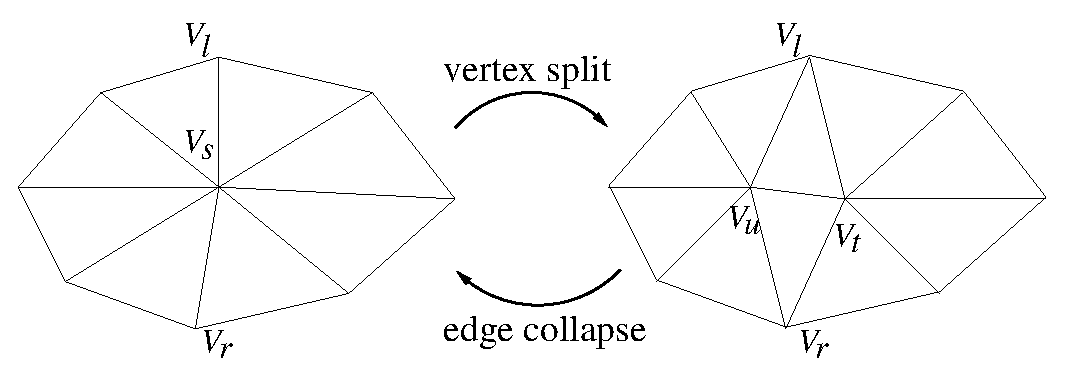
\epsfig{file = split.eps, height = 0.9in}
    \caption{Edge collapse and vertex split.
    This edge collapse removes one vertex by collapsing the edge $V_uV_t$ to a vertex $V_s$, and the
    vertex split reconstructs the edge from $V_s$. Vertices $V_l$ and $V_r$ are
    the cut neighbors of $V_s$.\label{dstream:split}}
    \end{figure}
    A commonly used representation of 3D models to support progressive streaming is
    progressive mesh \cite{237216}, which is based on two operations: 
    \emph{edge collapse} and \emph{vertex split}. 
    With the edge collapse operation,
    we can simplify a complex mesh into a simple base mesh
    by continuously collapsing one edge into
    a vertex. We reconstruct the original mesh
    by applying vertex split, the inverse of the edge collapse, in the
    reverse order of collapsing (see Figure \ref{dstream:split}). Therefore,
    progressive streaming can be implemented by sending the vertex
    splits as refinements after sending the base mesh.

    In progressive mesh streaming, it is desirable to increase the visual quality
    on the client side as quickly as possible.
    The ideal way is to send the vertex splits
    in the descending order of their contribution to
    mesh quality, commonly measured by the Hausdorff distance between
    the original and reconstructed mesh \cite{cignoni98metro}.
    As Hausdorff distance is view independent, 
    bandwidth may be wasted in sending invisible vertex splits
    before the visible ones. Moreover, even among the visible vertex splits,
    the view-independent metric cannot 
    reflect the real contribution to the visual quality of
    clients with different viewpoints. A vertex split that significantly
    changes a mesh may change the rendered image 
    only slightly.

    A better metric for visual contribution of a vertex split, which considers the receiver's viewpoint, is an image-based metric similar 
    to that proposed 
    by Lindstrom and Turk
    \cite{353995}, using the mean square error between the rendered images
    of the original mesh and reconstructed mesh.   
    %Lindstrom and Turk consider 
    %many viewpoints in their simplification since it is done off-line.
    %In the streaming case, we only need to consider the current viewer's
    %viewpoint. % since it is already known. Hence, 
    Based on this metric, \emph{view-dependent} streaming,
    in which vertex splits are sent in the descending order of 
    their contributions to the quality
    of rendered image, is introduced. 
    
    %can optimize the visual quality of the receiver side
    %during the transmission.
    %is a better choice.
    %because of two reasons. First, 
    %non-visible vertex splits will not be sent until all visible one are sent.
    %Second, the visible vertex splits can be sent in the descending order of 
    %their contributions to the quality of rendered image.

    \begin{figure}
    \centering
    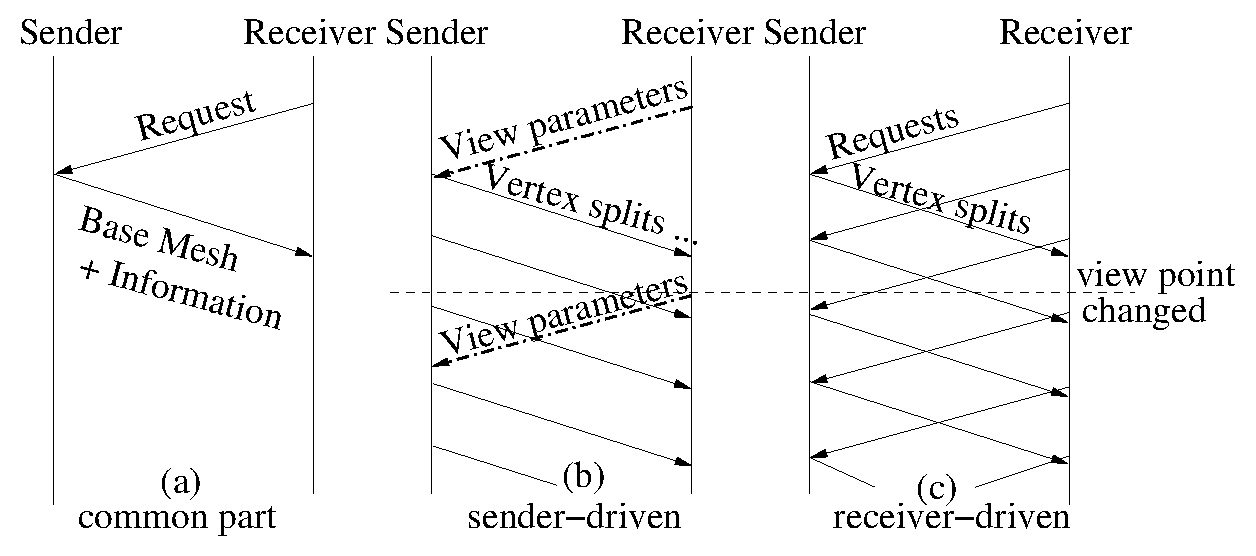
\epsfig{file = protocol.eps, height = 1.5in, width = 3.3in}
    \caption{Sender-driven protocol and receiver-driven protocol 
    \label{dstream:protocol}}
    \end{figure}
    In previous implementations of view dependent streaming
    \cite{To1999, 363375, progressive:Yang, kim:view, zheng:interactive}, 
    the server decides which vertex splits to send. In these implementations,  
    the client sends its
    viewing parameters to the server, and the server sends the chosen vertex splits after
    determining the visibility and the appropriate resolution of 
    different regions of the mesh (See Figure \ref{dstream:protocol}b).
    
    This sender-driven protocol, however, has two significant weaknesses.
    Firstly, it is not scalable to many receivers. Determining visibility of vertices
    and sorting the visible vertex splits based on their visual contributions
    are expensive operations. 
    %As a result, few of the existing schemes use sorting. In most implementations,
    %the visible vertex splits are sent in the reverse of collapse order, which is
    %often based on view-independent metrics. 
    Moreover, the sender needs to maintain
    the rendering state of each receiver to avoid sending duplicate data when receivers
    changes viewpoint.

    Secondly, due to the stateful design and huge computational requirements,
    the sender-driven approach cannot be extended easily to support 
    caching proxy and peer-to-peer architecture, two common solutions to scalability. It is not realistic
    to require each proxy or peer to provide much CPU time and memory. 
    Furthermore, a proxy or peer might not store the complete mesh.

    To address the above weaknesses, we propose a receiver-driven protocol,
    in which the receiver decides the sending order and explicitly requests
    the vertex splits. The sender simply sends the data requested 
    (See Figure\ref{dstream:protocol}c), so no expensive computation is needed.
    %In this protocol, the server is stateless and free of expensive computation.
    %We can exploit the client's GPU in determining the requesting order.
    Furthermore, the server is stateless, so
    existing cache proxy and peer-to-peer techniques can be applied.

    The receiver-driven protocol also reduces the size of data sent by the sender.
    In sender-driven protocols, for each vertex split, the sender has to send identifications
    to indicate which vertex to be split ($V_s$ in Figure \ref{dstream:split}),
    requiring at least $log_2{n}$ bits if $n$ vertices exist \cite{258843}. 
    In the receiver-driven protocol, however, the sender needs not send
    these identifications since the vertex splits can be sent according to
    the requesting order from the receiver. The identifications, sent
    by the receiver, consumes the down-link bandwidth 
    of the sender, which is often less likely to be the bottleneck than the up-link.

    Implementing the receiver-driven protocol is non-trivial. First, we need
    to assign each vertex a unique identification number so that the receiver
    can explicitly request vertex splits. Second, the receiver has to efficiently decide the
    importance of a vertex split based on partially received mesh.
    Although it is difficult for the receiver to accurately measure
    the visual importance of a vertex split, we find that estimation suffices
    in our scheme.  

    The main contributions of our work are as follows.  We
    propose a receiver-driven protocol of view-dependent streaming, which
    significantly reduces the CPU time of the sender
    and makes the sender stateless.  Our protocol exploits the receiver's 
    computing resources to approximate the optimal list of vertex splits to receive
    to improve the rendered mesh quality.  We also introduce an 
    algorithm to efficiently encode the receiver's requests.
    
    %Second, we reduce the transmission data
    %of the server by removing a significant part of data to its incoming channel. 
    %Third, we implement a prototype and evaluate its effectiveness with 
    %experiments.

    The rest of the paper is organized as follows.
    In Section \ref{s:dstream:related}, we introduce the related work. We briefly  
    review the traditional view-dependent approaches in Section \ref{s:dstream:terms}. 
    Then, we present the receiver-driven protocol 
    in Section \ref{s:dstream:protocol}.
    We evaluate our protocol in Section \ref{s:dstream:evaluation} 
    and conclude in Section \ref{s:dstream:conclude}.
\section{Related Work}
\label{s:dstream:related}
%\subsection{View-Dependent}
%\label{ss:view-dependent}
    The view-dependent approach first appeared as 
    a dynamic simplification method used for adaptive rendering of a complex 3D mesh
    \cite{258843, 258847}. Only vertex splits that contribute to the rendered
    image will be rendered, allowing real-time rendering of a complex mesh
    even with limited rendering capability.
    Besides progressive mesh, other multi-resolution representations, 
    such as vertex-clustering  and subdivision scheme,
    are used in view-dependent refinement systems \cite{245627, efficient:Alliez,602344}.

    Later, the view-dependent approach is used in progressive 
	streaming of 3D meshes.     In the scheme proposed by Southern et al. \cite{363375},  the client is stateless and
    maintains only the visible data. 
    To et al. \cite{To1999}
    and Kim et al. \cite{kim:view} proposed that received data are stored
    in the receiver even after they become invisible, 
    so they need not be resent when they are visible again. 
    In these papers, view-dependent approaches mainly aim at addressing
    limited rendering capability. 
    
    Yang et al. \cite{progressive:Yang} and
     Zheng et al. \cite{zheng:interactive}, on the other hand, use
     view-dependent streaming to address limited network bandwidth.
     Yang et al. proposed a scheme where the server chooses the appropriate resolution
     according to the available network bandwidth.
     Zheng et al. \cite{zheng:interactive} use prediction to
     reduce the effect of network latency and 
     compensate the round-trip delay with the rendering time.
     These systems use sender-driven approach and do not address
     server scalability issues.

    %\subsection{Reduce Dependency}
%\label{ss:reduce-dependency}
    The main challenge of these view-dependent schemes is 
    finding an appropriate subset of vertex splits to generate a 
    satisfactory rendered image on the client side.
    The flexibility of choosing a subset of vertices,
    hence, is crucial in view-dependent streaming. But this flexibility is
    restricted by the dependency among the vertex splits.
    For a manifold mesh, a vertex split operation depends on the existence of (a)
    the vertex to be split ($V_s$ in Figure \ref{dstream:split}), (b) two
    cut neighbors ($V_l, V_r$ in Figure \ref{dstream:split}). More dependencies exist if artificial
    folds are strictly forbidden \cite{258843, 258847}, but in this paper we
    ignore these dependencies since we can tolerate temporary folds in our scheme.

     To et al. \cite{To1999} further remove the second dependency.
     In their method, if a cut neighbor does not exist during a vertex split,
     its ancestor will be used as the cut neighbor instead.
     Kim and Lee \cite{kim01truly} improve this method so that the final mesh
     can keep the original connectivity. 
     %In their paper, when the original cut neighbor
     %is below the vertex front, its active ancestor is chosen instead. If the original
     %cut neighbor is above the vertex front, then we choose a proper active descendant of it.
     %As long as the two cut neighbors are not the same vertex, the vertex split can be processed.
     Kim et al. \cite{multiresolution:kim} propose a better scheme that enables
     an ordinary progressive mesh to be split in random order.
     This method is applied in our protocol to reduce the cut neighbor dependency
     and will be described in further details in Section \ref{s:dstream:protocol}.

     The flexibility in choosing split order, however, increases the difficulty
     in developing an effective encoding scheme. Most compression
     algorithms for progressive mesh %\cite{280834,319426, 614450, 383281,602153}
     choose a specific order of vertex splits
     to reduce redundancy by exploring the correlation
     between consecutive vertex splits.
     Moreover, compressed data can only be sequentially decoded
     so we cannot change the sending order. One solution
     proposed by Yang et al. \cite{progressive:Yang}
     is to divide the whole mesh into several segments and encode them
     separately to trade off between flexibility and compression efficiency.
     The weakness is that the size of the base mesh is relatively large
     since the original vertices in the border of segments are kept in the base
     mesh. Furthermore, the quality of the base mesh is uneven.

     Some related work \cite{multiresolution:kim, random:yoon}
     have proposed compression algorithms that allow random splitting of a mesh without
     sacrificing compression efficiency.   These algorithms are not designed for 
	 network transmission, but our scheme extended several ideas from Kim et al. \cite{multiresolution:kim}
     and applied them in view-dependent streaming.  

     The discussion above focuses on view dependent streaming of 3D meshes. View dependent streaming have also been used for other 3D data, such as terrain \cite{chang:terrains} and 3D scenes \cite{ott:tele}. 

\section{Current View-dependent\\ Approaches}
\label{s:dstream:terms}
    In this section, we briefly review the current view-dependent approaches since 
    they are the basis of our scheme.
   
    \begin{figure}
    \centering
    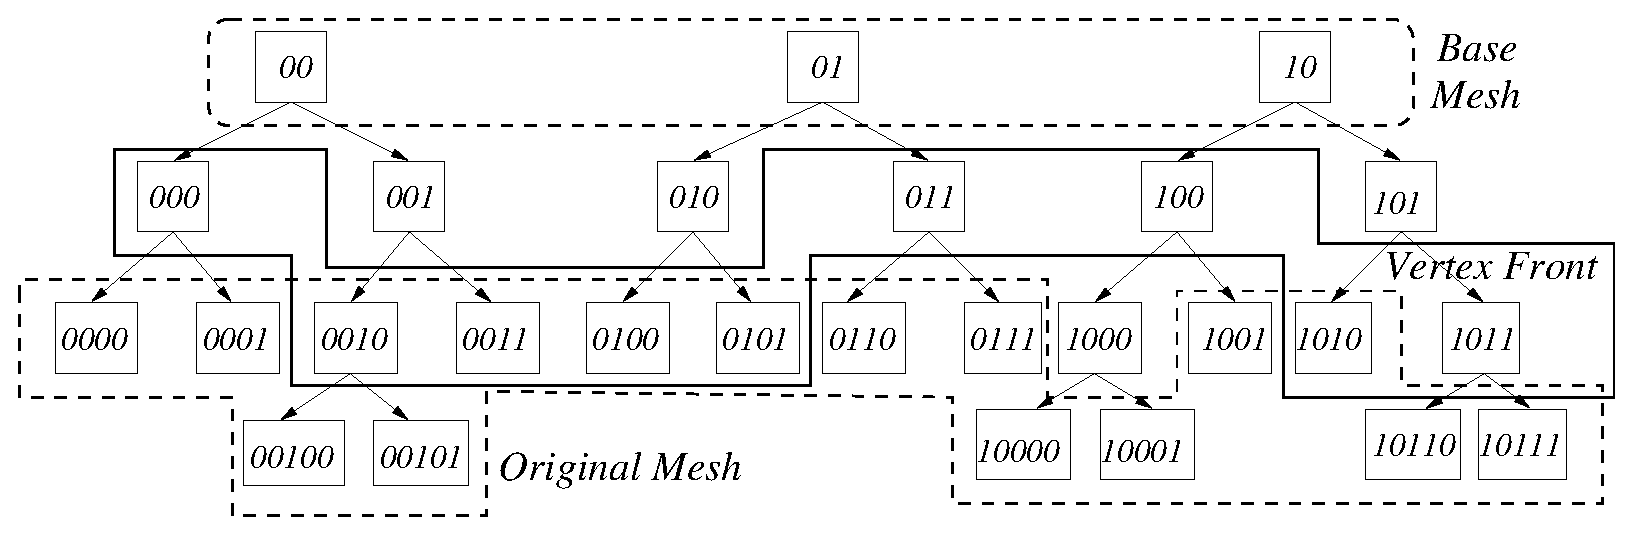
\epsfig{file = hierarchy.eps, height = 1.1in, width = 3.3in}
    \caption{Vertex hierarchy and vertex front. A rectangle represents a vertex and the number inside
    is its identification number, including tree ID and node ID.\label{dstream:hierarchy}}
    \end{figure}
    View-dependent systems often organize the vertices hierarchically.
    For example, Hoppe \cite{258843} represents
    parent-child relation among the vertices in a progressive mesh
    as a forest of binary trees, named \emph{vertex hierarchy},
    in which the root nodes are vertices in the base mesh, and
    the leaf nodes are vertices in the original mesh (see Figure \ref{dstream:hierarchy}).
    A vertex split replaces one vertex ($V_s$ in Figure \ref{dstream:split})
    by its two children ($V_u$ and $V_t$ in Figure \ref{dstream:split}).
    Thus, after applying some vertex splits,
    the result is a mesh lying between the original mesh and the base mesh.
    The set of vertices in current mesh is called \emph{vertex front}
    \cite{258843}
    (see Figure \ref{dstream:hierarchy}).% and vertices in the vertex front are \emph{active vertices}
    
    %When determining the visibility of vertex splits, a vertex split cannot be ignored when it
    %is not visible. If any of its descendants in the vertex hierarchy is visible,
    %the vertex split still needs to be applied. To avoid determining the visibility
    Due to dependencies among the vertices, visibility determination of a vertex cannot be based 
	on the vertex alone.
    An invisible vertex still needs to be split if any of its descendants is visible. 
    To avoid determining the visibility %\footnote{
    %For simplicity, in this paper determining the visibility also includes computing screen-space error.} for each
    recursively for all the descendants,
    %vertex in the vertex hierarchy is expensive. Therefore, 
    a common method is to use a bounding sphere to represent a vertex and all its descendants.
    Then, we can safely ignore a vertex split if its bounding sphere
    falls outside the view frustum.
    Similarly, a bounding cone of normal is used in back face culling \cite{258843}.
    %Therefore, some extra information to represent the bounding sphere
    %and bounding cone of normal is needed. Both Hoppe and Kim et al. \cite{258843, kim:view}
    %pre-compute the radius of the bounding sphere ($r_v$), the semi-angle of
    %the cone of normals ($\alpha$), and other two parameters
    %($\mu$ and $\delta$) for deciding the screen-space error
    %and store them with the vertex together.
    These bounding object-based methods are not appropriate
    in our receiver-driven protocol. First, it can only determine
    the visibility, but cannot sort the vertex splits by their visual contributions. 
    More importantly, the sender has to send
    these bounding parameters with the vertex splits, almost doubling 
    the data size.  We explain our solution to this issue in Section \ref{s:dstream:protocol}.
    %and the transmitted data size will be significantly increased. 
    %Since one vertex split has only five parameters, 
    %the identifications of two cut neighbors ($V_l$ and $V_r$) and the coordinations
    %of the new vertex ($x$, $y$, and $z$)
    %\footnote{We apply the half-edge collapse in our implementation
    %so that only coordinates of one vertex needs to be transmitted.},
    %adding four parameters almost doubles the data size. 
    %It is not acceptable since the network bandwidth
    %is considered as the main bottleneck.  

    After deciding the visibility, the sender sends the chosen vertex splits to the receiver.
    Six parameters are needed in a vertex split of a manifold mesh: the identification number
    (we call ID from now on) of the vertex to be split
    ($V_s$ in Figure \ref{dstream:split}) $Ids$, 
    the IDs for two cut neighbors 
    ($V_l$ and $V_r$ in Figure \ref{dstream:split}), $Id_l$ and $Id_r$,
    and the coordinates $x$, $y$, and $z$ of the right child ($V_t$ in
    Figure \ref{dstream:split}). Here, half collapse is used so $V_u$ remains at the same position
    of $V_s$. Many implementations use the sequence number of a vertex generated as its ID,
    but this method enforces the sender to be stateful since the sender has to remember 
    the sending order of each receiver.
    
    Kim and Lee \cite{kim01truly} proposed a new method, in which every vertex has
    an ID that is independent of the sending order. The ID of a vertex is a bit string
    with two parts: tree ID and node ID.
    Tree ID is the sequence number of the root of this tree in the base mesh, 
    and the node ID represents the path from the root to this vertex in the binary tree.
    For example, if the tree ID is `01', which is also the ID of
    the root vertex of this tree, the bit string `010' and `011' are the IDs
    of the left child and right child of the root vertex respectively. 
    A vertex hierarchy with the assigned IDs is shown in 
    Figure \ref{dstream:hierarchy}.
    
    Besides being independent of the sending order, another benefit of this scheme
    is that the IDs embed the hierarchy. Thus,  
    we can deduce the IDs of the ancestors and the descendants of each vertex. 
    For example, given `1001' as the ID of a vertex,
    we can deduce that `100' is the ID of its parent, `10010' is the ID of its left child and 
    `10011' is the ID of its right child. 
    This property frees the sender from sending the IDs of the two newly generated vertices
    ($V_u$ and $V_t$ in Figure \ref{dstream:split}), as they can be deduced by the receiver.
    
    The above property is also essential in splitting
    a progressive mesh in random order, in which the set of neighbors of a vertex
    during the decoding $\mathcal{N}'$ may not be $\mathcal{N}$, the set 
    during the encoding. If a cut neighbor with an ID of $Id$ %in $\mathcal{N}$
    is not in $\mathcal{N}'$, then either one of its 
    ancestors or at least one of its descendants must belong to $\mathcal{N}'$ \cite{multiresolution:kim}.
    In the former case, the ancestor is found and used as 
    the cut neighbor since its ID is the prefix of $Id$.  
    In the latter case, the descendants of the original 
    cut neighbor in $\mathcal{N}'$ are found since they all have $Id$ as their prefix.
    Kim et al. \cite{multiresolution:kim} propose a method to find out the 
    proper one as the cut neighbor and they show that despite using replacement
    in the vertex splitting, the original mesh can be 
    accurately reconstructed when all the vertex splits are applied.

    Kim et al. \cite{multiresolution:kim} also propose an algorithm
    to encode the IDs of two cut neighbors at about 12 bpv (bit per vertex) 
    and the coordinates $x$, $y$, and $z$ at about 21 bpv (with 12 bit quantization).
    Although their paper focuses on random access of local meshes, we find that this 
	method is useful in progressive streaming as well. 

\section{Receiver-Driven Protocol}
     \label{s:dstream:protocol}
	 We now present our proposed receiver-driven protocol
     for view-dependent progressive mesh streaming.
     We first introduce the process of transmitting 
     a progressive mesh. Then, we explain how the receiver decides the requesting order.
     Finally, we explain how we efficiently encode the request from the receiver.
     
     \subsection{Mesh Transmission} 
     A streaming session is initiated when the receiver requests for a specific
     mesh.
     The sender returns the complete base mesh and other necessary information
     (See Figure \ref{dstream:protocol}a) to the receiver.
     
     \begin{figure}
     \centering
     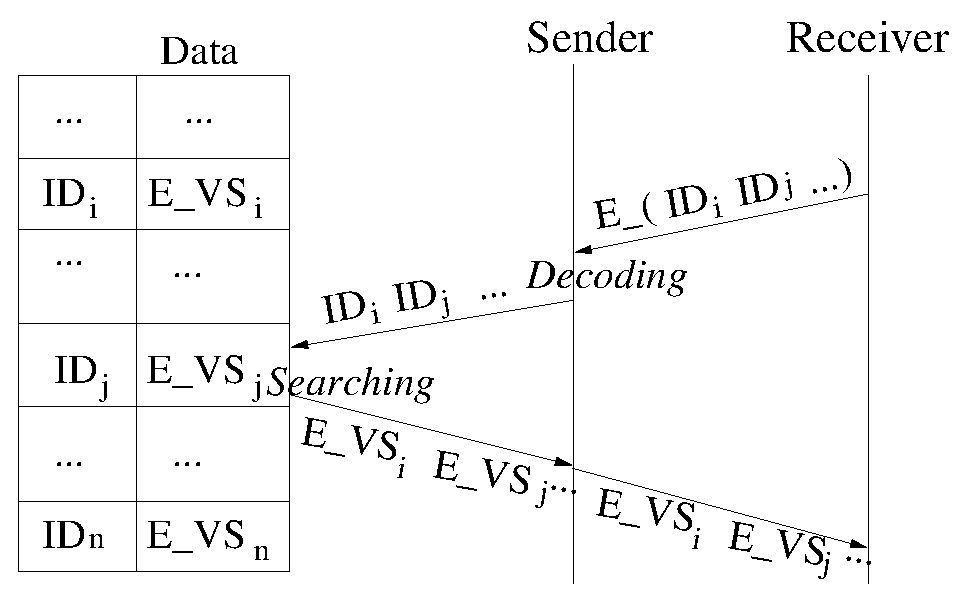
\epsfig{file =process.eps, height = 1.1in}
     \caption{The process of the sender in receiver-driven protocol. 
     E represents encoded data, and VS means vertex split. \label{dstream:process}}
     \end{figure}
     %After receiving the base mesh, 
     Then, the receiver determines
     the requesting order of the vertex splits based on the received base mesh, 
     encodes their IDs, and
     sends them to the sender. On the sender side, the vertex splits are stored
     in an associative array, which maps the ID to the vertex splits. 
     After receiving the encoded IDs from the receiver, 
     the sender decodes the IDs and searches for the vertex splits 
     in the associative array
     with IDs as the key values. The matched vertex splits
     are sent back to the receiver (See Figure \ref{dstream:process}). 
     The sender does only two things -- decode IDs and retrieve the 
     vertex splits, and is therefore stateless. 
     \subsection{Determining Visual Importance}
     \label{ss:dstream:visual}
     We now introduce how the receiver decides the requesting order. 
     We cannot directly use the mean square error between rendered images of 
     reconstructed mesh and original mesh to determine the order, 
     %image-based metric proposed by Lindstrom and 
     %Turk \cite{353995} 
     since we need to know the importance of a vertex 
     split before it is received. To overcome this problem, we estimate
     the importance of the vertex splits to request for based on the received
     mesh, using
     %We find that
     %estimation suffices %in the streaming case 
     %because some error in deciding the order will not affect the rendered
     %image.
     %
    \begin{figure}
    \centering
    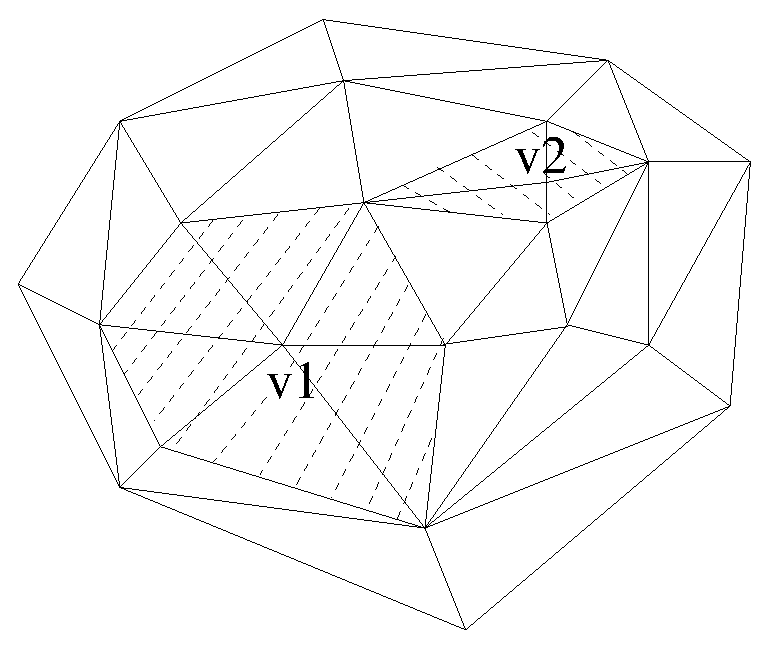
\epsfig{file =screen_area.eps, height = 1.0in}
    \caption{%Screen area of two vertices: v1 and v2.
    Rendered image on the receiver's screen. 
    The shaded are the screen area of vertex $V_1$ and vertex $V_2$.
    \label{dstream:screen_area}}
    \end{figure}
     %We use 
     the screen-space area of all the neighbor faces of a vertex as the 
     metric of its visual importance (see Figure \ref{dstream:screen_area}).
     The rationale is that if the screen area of a vertex ($V_1$ in Figure \ref{dstream:screen_area}) 
    is larger, it is likely the quality can
    be improved more by splitting this vertex. 
    Moreover, the screen-space area can be efficiently
    computed with the help of the GPU, by simply counting the
	number of pixels inside the faces in the frame buffer.
    %A simple method to compute the screen space of a triangle is 
    %to count how many pixels are inside it after rendering by analyzing
    %the frame buffer. 
    %We compute the screen-space area with the help of the GPU. 
    %First we assign each face in
    %the current mesh a unique color and render them. 
    %We can determine the visibility
    %and the screen-space area of each vertex by counting how many pixels with its color
    %are in the frame buffer, where the rendering result is stored. 
    %Then we add the pixel number to the face's three vertices. Thus, the
    %pixel number of a vertex (which is the sum of pixel numbers in its neighbor faces)
    %is proportional
    %to its screen-space area.
    %In brief, we estimate the visual importance of splitting a vertex by checking
    %at the projected area in the screen of the region occupied by this vertex and all its neighbors.
    
    Once the screen-space areas are computed, the receiver sends the requests 
	following the descending order of the 
    screen-space area. If the viewpoint changes, the visual importance will
    be re-computed and a new list of vertex splits will be requested. Since the received
    splits refine the mesh, the receiver recomputes the visual importance periodically
    to update the order even without viewpoint change. The refresh period, one second
    in our experiments, can be decided
    by the receiver based on mesh size and network bandwidth.

    The client can stop requesting once it finds that the rendering quality is sufficient.
    The receiver has the flexibility of continuing to request for the remaining vertex splits for future use.
    It can also pre-fetch some invisible vertices based on the prediction of future viewpoints.

    If the receiver stops requesting % for more vertex splits 
    when the visual quality is satisfactory, 
    it may miss some visible vertices since the visibility determination is just an estimate.
    Some invisible vertices may have potentially 
    visible descendants, but they will not be received if their parent has  
    no screen-space area. 
    Fortunately, in most cases, this kind of error is small and 
    tolerable (See the experiment results in Section \ref{s:dstream:evaluation}).
    If strict accuracy is needed, the receiver can choose to continue requesting 
    for the remaining vertex splits.  
		%Furthermore, some methods may reduce 
    %this kind of error, for example, by generating an appropriate base mesh or giving more
    %weight to the silhouette. We will consider these techniques in the future. 
    \subsection{Encoding of Vertex Splits and IDs}
    \label{ss:dstream:encoding}

    %Our progressive meshes are generated using OpenMesh\footnote{http://www.openmesh.org}. 
    %Here, we consider only manifold meshes and use half collapse in the simplification. We 
    %%The happy Buddha mesh is from Stanford University.
    %also use Kim's algorithm \cite{multiresolution:kim}
    %to code the IDs of two cut neighbors ($Id_l$ and $Id_r$).

	In this section, we explain how we encode the vertex splits 
	and the IDs of the requested vertex splits.  Note that, in 
	our work, we consider only manifold meshes and use half 
	collapse in the simplification.
    
	To encode a vertex split, we need to encode the IDs of the two
	cut neighbors and its $x$, $y$, and $z$ coordinates.
	We use Kim's algorithm \cite{multiresolution:kim} to code
	the IDs of the cut neighbors.
    To encode the coordinates, instead of encoding $x$, $y$, and $z$ directly, we encode $dx$, $dy$, and $dz$ with
    Huffman coding algorithm. Here $dx = x - x_0$, $dy = y - y_0$,
    and $dz = z - z_0$, and $x_0$, $y_0$, and $z_0$ are the coordinates of
    $V_s$, the vertex to be split. 
    The rationale to code the differences is that they have less entropy, especially
    for the later part of vertex splits, which only change the coordinates slightly.
    It is worth noting that all the encoding process are done off-line and the 
    encoded vertex splits are stored in the associative array, so the encoding will
    not increase overhead to the sender.

    According to the results of our experiments with the Stanford Happy Buddha model,
    we can quantize $dx$, $dy$, and $dz$ to 14 bits. 
    We need 11 bpv for both $Id_l$ and $Id_r$ 
    and 20 bpv for all three of $dx$, $dy$, and $dz$ on average.
    It is worth noting that more bits are needed for $dx$, $dy$, and $dz$ 
    for the earlier vertex splits (about 30 to 35 bpv)
    since their values are larger. 
    The number of bits needed decreases significantly for later part of the vertex splits
    as $dx$, $dy$, and $dz$ decrease. We think that compressing $x$, $y$, and $z$ 
    based on better prediction techniques may further increase the 
    efficiency and it will be an interesting topic of future work.

    We now introduce how we encode the vertex split IDs, 
    which need 32 bpv without compression.  
    %First we choose the number of vertex identifications to be packetized appropriately
    %such that their vertex splits after encoded will no exceed
    %the size of an Ethernet packet (often 1500 bytes). The reason is to
    %reduce the dependency among packets so that
    %one packet loss will not affect the decoding of another packet.
    %A previous paper \cite{1291399} has discussed the importance to reduce the dependency
    %among the packets.
    The two parts of an ID, tree ID and node ID, are encoded separately.  We use a bit string \textit{code} to store the encoded result.
    First, we sort the IDs in a packet according to the tree IDs, in increasing order. 
    Then, we store the first tree ID to \textit{code} and 
    store each of the following tree ID as the difference from the previous tree ID.
    Since they are sorted, the differences are positive and relatively small numbers.

    \begin{figure}
    \centering
    \epsfig{file =encode_id.eps, height = 1.0in}
    \caption{The code of ID of the bottom two
    vertices is 1011001000. 
    \label{f:dstream:encode_id}}
    \end{figure}
    \begin{algorithm}
    \caption{Encoding Vertices in One Tree.
    Input: IDs of vertices in a tree to be split;
    Output: a bit string as the \emph{code}.\label{a:dstream:encode_id}}
    \begin{algorithmic}
    \IF{no vertex needs to be encode in the left subtree}
        \STATE append `0' to \emph{code};
    \ELSE
        \STATE append `1' to \emph{code};
        \STATE encode the left subtree;
    \ENDIF
    \IF{no vertex needs to be encode in the right subtree}
        \STATE append `0' to \emph{code};
    \ELSE
        \STATE append `1' to \emph{code};
        \STATE encode the right subtree;
    \ENDIF
    \end{algorithmic}
    \end{algorithm}
    Next, we encode the node IDs in a tree into a bit string with 
    a recursive algorithm (See Algorithm \ref{a:dstream:encode_id}).
    In brief, we use two bits to represent whether one or more descendants need
    to be split (`1' for yes and `0' for no)
    in the left subtree and right subtree respectively. 
    In the example shown in Figure \ref{f:dstream:encode_id}, for the root vertex, since at least one vertex
    in the left subtree needs to be split, we append `1' to the code and encode the
    left subtree. At the root of the left subtree, since no vertex needs to split in its left
    subtree, we append `0' and check its right subtree. Vertices to be split exist in the right
    subtree, so we append `1' and encode its right subtree recursively as `100100'. 
    Finally, we return back to the root and append `0' since 
    no nodes in the right subtree needs to be split. 
    Therefore, the result is `1011001000'.
        
    During decoding, the sender traverses the tree according to the bits of the code. 
    The bit `1' means to decode the subtree and the bit `0' means to stop and return.
    If a vertex has no descendants that needs to be decoded, then this vertex is split. 
    Decoding is done when the procedure returns to the roots.
    
    The advantage of this method is that the code length is variable and the 
    length can be determined without extra flags. The coding efficiency depends
    on how many vertices need to be split inside a tree. Two bits
    are assigned to each vertex traversed during the encoding
    (including the vertices to be split and their ancestors in their path
    to the roots). Thus, the code efficiency is higher when more vertices in one tree
    are encoded since the overhead is amortized across the vertices. 
    %In worst case, we traverse $d$ nodes just for encoding $1$ vertex,
    %so in maximum $2d$ bits are needed for a node ID. Here, $d$ is
    %the depth of a node. In best case, all leaves are needed to be split. 
    %Assuming there are $m$ leaves, then the
    %total traversed nodes are $2m-1$ and the total bits are $4m-2$.
    %Therefore, in minimum about $4$ bits is needed
    %to encode a node ID. 
    %
    %Due to the limited space, we omit the decoding algorithm
    %here. It can be deduced from the encoding algorithm.

    We can further reduce the data size for some receivers whose up-link (receiver to
    sender link) bandwidth is much less than the down-link (sender to receiver link) 
    bandwidth. These receivers can request the sender to send not only the vertex split
    for the requested vertex but also the vertex splits for its descendant.
    For example, if the receiver sends an ID 
    `10010', the sender can send vertex splits for `10010', `100100', `100101'.
    The receiver can explicitly indicate in the packet how many descendants to send. This method 
	also allows the server to better utilize its outgoing bandwidth by filling the pipeline when RTT between the server and the client is high.

\section{Evaluation}
In this section, we introduce the experiments results to evaluate our protocol.
We choose two computers on a LAN as the sender and the receiver. 
We use several meshes from Stanford University in our experiments, but we only
present the result of Happy Buddha in this paper due to the space limit.
\label{s:dstream:evaluation}
\subsection{CPU Usage of the Sender}
\begin{table}[b]
\centering
\begin{tabular}{|c|c|c|}
\hline
&Sender-driven &Receiver-driven\\
\hline
send    base mesh           & 1.40s & 1.13s  \\
%receive encoded IDs         & -     & 0.06s  \\
decode  IDs                 & -     & 1.55s  \\
search vertex split         & 1.85s  & 1.85s \\
%receive the view parameters &       & -      \\
%traverse vertex hierarchy   &   & - \\
determine visibility        & 0.41s & - \\
update vertex front         & 1.41s & - \\
encode IDs                  & 0.94s & - \\
%send data                   &       & 0.10s  \\
others                      &0.16s  & 0.16s\\
\hline
\end{tabular}
\caption{Comparison of CPU usage of the sender.
\label{t:dstream:cpu}}
\end{table}
We compare the CPU usage of the sender in sender-driven
protocol and receiver-driven protocol after all vertex splits
are received (see Table \ref{t:dstream:cpu}). 
The implementation of the sender-driven protocol is modified from
our receiver-driven protocol using the visibility determination
algorithm from Kim et al. \cite{kim:view}. % by adding encoding scheme.
In both experiments, the client changes its viewpoints exactly the
same way.
A computer with an Intel Core 2 Duo 2.4 GHz CPU and 4 GB memory is
used as the sender.  We profile the code five times 
with Google CPU profiler and take the average value.
%We transmit
%the Stanford Happy Buddha mesh with both protocols and compare
%the CPU time used by the servers. 
We can see that the receiver-driven protocol reduces the CPU usage
of the sender by 24\% since we remove the processes for determining the visibility and updating the vertex front on the sender. 
\subsection{Transmitted Data Size}
During transmissions of the Happy Buddha model (542652 vertex splits) using 
the receiver-driven protocol, 1.83 MBytes are sent from the receiver
to the sender as vertex split IDs, and 2.21 MBytes are sent from the sender 
to the receiver as vertex splits. 
Thus, on average, IDs cost 27 bpv and vertex splits cost 32 bpv.
If sender-driven protocol is used, both IDs and 
vertex splits are sent from the sender to the receiver, so the total data 
sent by the sender are 4.04 MBytes. Thus, by moving IDs from the down-link to up-link, we reduce the outgoing bandwidth consumption of the sender by more than 40\%.

Reducing the outgoing data size also shortens the downloading time.
In the receiver-driven protocol, although the total transmitted size remains
the same, about 40\% of the data are now transmitted in the up-link of
the client.  On duplex links where up-link transmission can occur concurrently with down-link
transmission, the total transmission time reduces by about 40\% as well.
%\footnote{Recall that users with low up-link bandwidth can request a packet with its descendants at once to reduce the up-link data rate.}. 
%Assuming that the server keep sending data at $R$ Bps, IDs cost $S_i$ bytes,
%and Vertex splits cost $S_v$ bytes. Then sender-based protocol needs
%$t_s = \dfrac{S_i + S_v}{R}$ to download the mesh, but the receiver-driven protocol
%needs only $t_d = \dfrac{S_v}{R} + t$, where $t$ is the time to send the first several
%packets of IDs before the first packet of vertex splits arrive,
%since the sending of remaining IDs are parallel with the downloading. 
%Because $t$ is much less than $\dfrac{S_v}{R}$, $t_d$ is much shorter than
%$t_s$. 
\subsection{Quality}
%   \begin{figure}
%    \centering
%    \epsfig{file =psnr.eps, height = 2.6in, angle = 270}
%    \caption{
%    Relation between PSNR value and received vertices\label{f:psnr_vertices}}
%    \end{figure}
%In progressive streaming, the optimal sending order generates
%the fastest growing of rendered image quality. Therefore,
%we check the effectiveness of our protocol by checking the
%quality increasing curves. We choose the PSNR value as the 
%metric of rendered image quality. In Figure \ref{f:psnr_vertices}, 
%we can see the relation between PSNR value and the received vertices
%number. The view-independent streaming sends a lot of invisible vertex splits, 
%so the quality increases much slower than the view-dependent streaming.

   \begin{figure}
    \centering
    \epsfig{file =vps2.eps, height = 2.6in}
    \caption{
    The upper row shows the rendered images, and the lower row shows 
    the reconstructed meshes when the quality of rendered images is acceptable.
    %For each mesh, left: front side, right: back side.
    The rectangles over the images represent the viewable areas of the user.
    \label{f:dstream:vps}}
    \end{figure}
   \begin{figure*}
    \centering
    \begin{tabular}{ccc}
    \epsfig{file =psnr2.eps, height = 2.2in, width = 1.5in, angle = 270}
    &
    \epsfig{file = psnr22.eps, height = 2.2in, width = 1.5in, angle = 270}
    &
    \epsfig{file = psnr23.eps, height = 2.2in, width = 1.5in, angle = 270}
    \\
    \\
    View Point 1
    &
    View Point 2
    &
    View Point 3
    \\
    \end{tabular}
    \caption{
    How PSNR changes with amount of received data.  We cut off the curve when PSNR = 35 as its value approaches infinity when enough data are received.
    \label{f:dstream:psnr_bytes}}
    \end{figure*}
We follow Lindstrom and Turk \cite{353995} and use an image-based metric
to evaluate the quality of a reconstructed mesh. It is reasonable since
the representation of a 3D mesh on the receiver side is the 2D rendered image.
In this paper, we use the PSNR value of the rendered image as the metric,
with the rendered image of the original mesh as the reference. 

Figure \ref{f:dstream:psnr_bytes} shows how PSNR changes with the amount of data received. 
Assuming constant transmission rate, this figure
also shows how PSNR value changes with time. 
We do the experiments with three different viewpoints (see Figure \ref{f:dstream:vps}). 
In receiver-driven protocol, the quality grows much faster than sender-driven protocol because 
data transmitted are reduced.
View-independent streaming, although having the highest 
compression ratio (20 bpv \cite{383281}), 
wastes majority of bandwidth in sending invisible
vertex splits, so it increases the quality at a slower rate, 
especially when only a small part of the mesh is visible (e.g. View Point 3). 

\if 0
\begin{table}
\centering
\begin{tabular}{|c|c|c|c|}
\hline
       & receiver-driven & sender-driven & view-independent\\
\hline
viewpoint1 &    718K     &   1383K      &     1332K       \\
\hline
viewpoint2 &    267K     &    511K      &     1302K       \\
\hline
viewpoint3 &    113K     &    200K      &     1280K       \\
\hline
\end{tabular}
\caption{The bytes needed to achieve PSNR > 30.\label{t:dstream:psnr30}}
\end{table}
Now we assume PSNR value being 30 as the acceptable quality. Table \ref{t:dstream:psnr30} shows
the bytes needed to be received to achieve the acceptable quality, and Figure \ref{f:dstream:vps}
shows the rendered images and reconstructed meshes.
Table \ref{t:dstream:psnr30} shows that our protocol can achieve the acceptable quality much quicker. 
\fi
\begin{table}
\centering
\begin{tabular}{|c|c|c|c|}
\hline
             & View Point 1 & View Point 2 & View Point 3 \\
\hline
error pixels &   305           &      226       &     115         \\
\hline
proportion   & 0.12\%             &   0.09\%           &  0.05\%           \\
\hline
PSNR         &   37.8        &    38.3        &    40.6        \\
\hline
\end{tabular}
\caption{Errors of rendered mesh when only visible vertices are split.
There are 250,000 (500$\times$500) pixels in total.\label{t:dstream:error}}
\end{table}
As we explained in Section \ref{s:dstream:protocol}, if the receiver stop requesting vertex splits after all the visible splits received,
some potentially visible vertices may not be generated.
We use two methods to compare the rendered images between the original mesh and the reconstructed mesh when all visible vertices
are split. One is to find
how many pixels are different and the other is to compute the PSNR value. 
Table \ref{t:dstream:error} shows that the error is negligible.
% -- less than 0.12\% of the pixels are different and the PSNR values of the rendered images are at least 37.8.
%add figures and explanation here.
\section{Conclusion}
\label{s:dstream:conclude}
\if 0
In traditional view-dependent systems,
senders decide which refinements to send, so they are
stateful and need expensive computation. %Not only the CPU time but also
Besides the CPU time,
the output bandwidth also make the sender not scalable to many receivers,
since cache proxy and peer-to-peer system cannot be applied easily.

We propose a receiver-driven protocol to address the above weakness.
The main finding of us is that %the accuracy of rendered image is not
%strictly required during previewing,
receivers can estimate the visual importance of a vertex split, even before
it is received, based on the current received mesh. Moreover, we can exploit the GPU
in determining the visibility and visual importance of vertices.

In our protocol, the sender is stateless,  so the receiver can easily
switch from different senders during transmission or even simultaneously
download from multiple senders. Therefore, we can easily apply
the cache proxy or peer-to-peer techniques to solve the scalability problem. 

Another benefit is that the receiver explicitly requesting the vertex splits
frees sender from sending the IDs of vertex splits. As a result, the
transmission data on the down-link of the sender is significantly reduced. 
\fi
In this paper, we propose the receiver-driven approach for view-dependent 
streaming of 3D meshes.  Our preliminary study shows that the approach
is promising in reducing the sender's resource requirements, both in CPU and
outgoing bandwidth.  The stateless nature of the sender in our approach makes
it a natural choice in peer-to-peer mesh streaming and caching proxy.
We plan to study how our protocol can be applied in these two areas.  Our
protocol can also be easily extended to support streaming of a scene with
multiple mesh objects.
%This paper is the first step in receiver-driven approach
%and many improvements can be done in future. 
%For example, better visual importance estimating algorithms may be
%developed later. Progressively improving the geometrical precision
%may be used to reduce the bandwidth requirement in the initial
%stage. Peer-to-peer system of progressive mesh streaming can be
%designed based on our idea. Moreover, our scheme can be further
%extended to progressive streaming of a complex scene instead of just one
%object. 
\section*{Acknowledgment}
This work is supported by National University of Singapore Academic Research Fund R-252-000-306-112.

\chapter{Characterizing and Modeling User Interaction with Progressively Transmitted 3D Meshes}
\label{c:user}
\section{Introduction}
High-resolution 3D meshes are typically data rich and demand high network bandwidth 
and computational power. 
When these meshes are viewed on portable devices with
low bandwidth and slow CPUs, delays in both transmitting and
rendering become unavoidable. To minimize negative user experience, the
streaming system needs to prioritize data chunks according to user needs and
efficiently cache the most frequently viewed data.  Designing such
systems requires a thorough understanding of user behaviors in viewing 3D
meshes.

Moreover, if we could derive certain pattern in users' interaction with
high-resolution meshes, we could create a large number of synthetic traces,
which simulate users' actions, and these traces can be used in modeling system
performance during simulations. This method is much cheaper than collecting 
a large number of traces from real users and can be used in developing and evaluating
prototypes. For example, we use the synthetic traces we generated to test our P2P mesh
streaming systems introduced in next Chapter.

Most previous work on user interactions with 3D objects
focused on design of specific interaction
techniques
(e.g., the study by Chen et. al \cite{chen88study} and Hinckley et. al \cite{hinckley97usability}). 
In this thesis, however, we study
user behavior from the system design point of view, 
such as predictability (for pre-fetching) and locality of access patterns (for caching),
similar to the spirit of the landmark studies for the Web \cite{huberman98web} and file system \cite{ousterhout85trace}.  
No such prior study exists for progressive meshes. This chapter presents our first step towards filling 
this gap.

We conducted a user experiment\footnote{Thanks for Ransi De Silva for conducting this experiment.}
with 37 users interacting with 9 meshes.
We log the user's actions while they interact and view the meshes in a mock online shop.  
We present the analysis of these traces in this paper\footnote{Dan Liu helps in part of the analysis (session time,
think time, and predictability).}, 
and highlight findings that are significant to the design of efficient 
and scalable progressive mesh streaming systems.  
In particular, we found that 
(i) in certain scenarios, user actions are highly predictable, making pre-fetching useful in these cases; 
(ii) users' viewpoint concentrates on part of the meshes, making caching these popular spots useful. 
We also develop a simple model, which can be used to generate synthetic traces for evaluating large-scale progressive mesh streaming systems.
\begin{figure}[htp]
\centering
\begin{tabular}{cc}
    \epsfig{file=figs/thai, height = 0.6\textwidth} &
    \epsfig{file=figs/happy, height= 0.6\textwidth} \\
    Thai Statue &
    Happy Buddha \\
\end{tabular}
\epsfig{file=figs/dragon, width = 0.7\textwidth} \\
Dragon
\caption{Meshes used in experiment.   
Thai Statue (5 million vertices), Dragon (3.6 million vertices), and Happy Buddha (0.5 million vertices).}
\label{fig:3dmodels}
\end{figure}

\section{User Study}
\label{s:user:study}
\textbf{Meshes}

Three 3D meshes are chosen from the freely available
Stanford 3D Scanning Repository\footnote{http://graphics.stanford.edu/data/3Dscanrep/}:
\textit{Happy Buddha}, \textit{Dragon}, and \textit{Thai Statue}.
These meshes vary in complexity (amount of vertices), orientation, and
symmetry in space from default viewing direction. \textit{Happy Buddha} is the
simplest, is vertically oriented, and has a default viewing direction
orthogonal from the face of the Buddha. From that direction, the mesh is
asymmetric between front and back. The geometric shape of \textit{Happy Buddha} is
somewhat representative of all human-like statues. \textit{Dragon} is more complex
and is horizontally oriented. The default viewing point is from one
side of the body. Unlike \textit{Happy Buddha}, it is front-back symmetric
relative to the default viewing direction. The geometric shape of \textit{Dragon} is
somewhat representative of most mammals. \textit{Thai Statue} is the most complex
and is actually a compound mesh composed of three identical sides, each 
with three different objects: a Goddess, an elephant, and a dragon,
stacking vertically from top to bottom.  These three sides connect to
form a triangular cylinder. There are three possible default
viewing directions, one each from three corners of the triangular mesh. The
\textit{Thai Statue} is included as an example of complex compound mesh.

We replicate each mesh above twice, generating nine meshes in total.  
We added one localized visual defect, by denting a small region, to each replicated mesh 
without changing its number of vertices or faces. The reason for adding the defects will be explained later. 
The location and nature of the
defects vary between the meshes. As \textit{Happy Buddha} is
relatively simpler and has a smooth surface, its defect is
 more obvious than \textit{Dragon}
and \textit{Thai Statue}.  Defects for the later two meshes, due to the
irregular surfaces, are hard to find unless the user zooms in
considerably.

The meshes are encoded progressively and streamed over a simulated network of 320Kbps and 400ms round trip time.  

\textbf{Participants.}

A total of 37 (25 male and 12 female) participants, aged 19 to 36
(mean 23), mostly from the university community participated in the
experiment. None had any visual handicaps.

\textbf{Design and Procedure}

Our experiment mimics the following general real world scenario. Customers
are shopping in an online antique store. Each product in the store has a
number of items, and each item is represented by a 3D mesh closely resembling
the corresponding real world item. These items vary in quality, and some
have visible defects. Before purchasing, customers will carefully examine the
available items for a product in order to pick the best item available for
that product category.

We designed our experiment using a simple case of the above scenario. 
Our online store has three different products,
corresponding to the three different meshes mentioned earlier. Each product
has three available items in varying quality. Two of them have visual
defects (note: defects are created without changing any mesh
characteristics). Due to the different complexity of each mesh, the defects
are easier to find in the simpler meshes (\textit{Happy Buddha}) compared to the more
complex ones (\textit{Thai Statue} and \textit{Dragon}).

\begin{figure}
    \centering
    \epsfig{file=online_shop.eps, width = 0.85\textwidth}
    \caption{The user interface we used to mimick an online shop.}
    \label{f:user:shop}
\end{figure}
The participants were first instructed about the keyboard commands 
to view and interact with the 3D meshes, and given brief practice of
these commands on a simple mesh before starting the experiment. The
participants were presented with an user interface mimicking an online
catalog with three products (see Figure \ref{f:user:shop}).  For each product, images of three items 
(i.e., three versions, one original and two with defects) are shown on the screen.
The order of the products are randomized to avoid order effects.
The participants' job is to pick the best item among the three. Each item 
can be viewed in any order and if desired, multiple times.  When 
a participant selects an item, a new viewing window (width of 14cm and
height of 15cm, with a resolution of $500 \times 500$ pixels) opens, and the 3D mesh corresponding to that item is
progressively streamed and rendered in the window.  
The participants can interact freely
with the mesh until they close the window.
They would mark the item to be purchased after viewing all three items and
move on to the next product. Each participant must go through all three products to
complete the experiment.

\textbf{User Behavior Logs}

During the experiment, users' key press actions and viewpoints
were logged for off-line analysis. The representation of the viewpoints
and actions are introduced in detail as follows.

A viewpoint indicates from where and to which direction users view the mesh.
Users can change their viewpoints during the session. Changing the position of 
viewpoint is equivalent to changing the position of the mesh. 
%Therefore, from another aspect,
%users are changing the position and direction of the mesh during the session.
When the application starts, the user begins with the default viewpoint,
where the user looks at the center of the mesh (more precisely,  the center of the bounding box of the mesh)
from a distance far enough to see the whole mesh. 

We use a 6-tuple, ($x, y, z, \theta_x, \theta_y, \theta_z$) to indicate the relative position of the mesh,
%The ($x, y, z, \theta_x, \theta_y, \theta_z$) means
when the mesh is translated $x$ units right, $y$ units up, and $z$ units closer to the user (i.e. out of the screen),
and rotated $\theta_x$ degrees around $x$ axis, $\theta_y$ degrees around $y$ axis,
and $\theta_z$ degrees around $z$ axis. 
%During the rotation, the center of the mesh is not moved.
The positive directions of translation and rotation are shown in the Figure \ref{f:user:viewpoint}.
The default position is ($0, 0, 0, 0, 0, 0$).
\begin{figure}
    \centering
    \epsfig{file=viewpoint.eps, width=0.3\textwidth}
    \caption{The positive direction of translation and rotation.}
    \label{f:user:viewpoint}
\end{figure}
The position of $x$, 
$y$, and $z$ changes in unit equivalent to one tenth of the bounding length, which is the edge length
of the bounding box of the mesh. The angles of $\theta_x$, $\theta_y$, and $\theta_z$ change in unit of 10$\degree$,
and their range is $[0, 1, \cdots, 35]$.

To facilitate the analysis, we ensure the six values are all integral. 
Therefore, an action will change one of the six values by one unit.
Table \ref{t:user:action} lists out the name, the abbreviation, the result,
and the corresponding key (or key combination) of each action.\footnote{
There is a small inconsistency in our design. 
We use $\uparrow$ to move the mesh closer and $\downarrow$ to move the mesh
further. It is more like moving viewpoint than moving the mesh. 
It is the flaw in our design, but fortunately the users were used to it quickly
during the experiments.}
%When moving and zooming, 
%we move the viewpoint of the user, 
%but when rotating, we rotate the mesh. 
%In other words, when we press ALT + $rightarrow$, 
%we move ourselves to the right side of the mesh. 
%When we press $rightarrow$, however, we revolve the statue to right. 
%Fortunately, users accept this setting well and without confusion.}.

\begin{table}
    \centering
    \begin{tabular}{|c|c|c|c|c|}
        \hline
        Name & Abbreviation & Result & key/key combination \\
        \hline
        move right & MR     & $x + 1$  & ALT + $\rightarrow$\\
        move left  & ML     & $x - 1$  & ALT + $\leftarrow$\\
        move up    & MU     & $y + 1$  & ALT + $\uparrow$\\
        move down  & MD     & $y - 1$  & ALT + $\downarrow$\\
        zoom in    & ZI     & $z + 1$  & $\uparrow$\\
        zoom out   & ZO     & $z - 1$  & $\downarrow$\\
        tilt backward & TB  & $\theta_x + 10\degree$ & CTRL + $\downarrow$\\
        tilt forward & TF   & $\theta_x - 10\degree$ & CTRL + $\uparrow$\\
        revolve anticlockwise & REAN & $\theta_y + 10\degree$ & $\rightarrow$\\
        revolve clockwise & RED & $\theta_y - 10\degree$ & $\leftarrow$\\
        rotate  anticlockwise & ROAN & $\theta_z + 10\degree$ & CTRL + $\leftarrow$\\\
        rotate  clockwise & ROC &  $\theta_z - 10\degree$ & CTRL + $\rightarrow$\\
        %reset      & RS     & $all = 0$  & R \\
        quit       & Q      & quit     & Q \\
        \hline
    \end{tabular}
    \caption{Introduction of the actions.}\label{t:user:action}
\end{table}


As a result, a user session can be seen as a random process 
with viewpoints as the states. Each action transits
the system from one state to next state, until the QUIT
action terminates the session (see Figure \ref{f:user:transition} as an example). 
During the session, we record
all the user actions and the time they happened.  We call these 
records \textit{user trace}.
Moreover, ($x, y, z, \theta_x, \theta_y, \theta_z$) can be seen as a point in a 6-dimension space, and
the six axises in this space are $X$, $Y$, $Z$, $AX$, $AY$, $AZ$. 
In this sense, a session is a random walk in the 6-dimension space.
\begin{figure}
    \centering
    \epsfig{file=transition.eps, width=0.7\textwidth}
    \caption{An example of a user session}
    \label{f:user:transition}
\end{figure}


\section{Results and Implications}
In this section, we present our analysis on the user behavior. We present only on the analysis of the original (non-defect) statues, unless otherwise specified.
In addition, we also discuss what implications these results have on system design.

\subsection{Session Length}
\label{ss:user:session}
Session length refers to the time each user spends in viewing a mesh. 
Generally, the session length is short, with the average values of 107s, 76s, 47s for \textit{Thai Statue}, 
\textit{Dragon}, and \textit{Happy Buddha}, respectively (see Table \ref{t:TimeTable}). 
Figure \ref{fig:session-length}(a) shows the distribution. 
The session length decreases with complexity of the meshes, as expected. 
The session length fits the \textit{log-normal} distribution.

%The three models show different distributions. Such results are expected, for the session length is related to the users' interest in the models and the levels of details in different models.  Among these three models, Thai Statue is the biggest one, which provide the most coarse model to users when users start to view it, while ``Happy Buddha`` is the smallest one with less interesting details in it. 
%In generaly, the results of the session length distribution gives us two implications. First, the session length is short with maximum value of $376 sec$, which increase the difficulty in data sharing in P2P 3D mesh streaming systems. Second, the session length is dependent on the content of the models, and thus we need to consider the different features of the content of the model when generating synthetic traces for them.

\begin{figure}[htp]
\begin{center}
\begin{tabular}{cc}
\epsfig{file=figs/unconditionalThinkTimeResults/sessionLengthdistribution.eps, width=0.45\textwidth,angle=270}&
\epsfig{file=figs/unconditionalThinkTimeResults/Inter-operationTimeDistribution.eps, width=0.45\textwidth, angle = 270}\\
\end{tabular}
\caption{\label{fig:session-length} (a) Session Length and (b) Inter-stroke Time}
\end{center}
\end{figure}

%\begin{figure}[htp]
%\begin{center}
%\epsfig{file=figs/RegionType0/sessionLengthdistribution.eps, width=0.28\textwidth, angle = 270}
%\caption{The Session Length Distribution}
%\label{fig:session-length}
%\end{center}
%\end{figure}

\begin{table}[hbp!]
\begin{center}
\begin{tabular}{|c|c|c|c|c|c|}
\hline 
Mesh&\multicolumn{2}{c|}{Session Length}&\multicolumn{2}{c|}{Think Time}\\
\cline{2-5}
&Mean($s$)&Max($s$)&Mean($ms$)&Max($s$)\\
\hline
Thai Statue&107&376&593&25\\
\hline
Dragon&76&272&574&20\\
\hline
Happy Buddha&47&98&403&13\\
\hline
\end{tabular}
\caption{Session Length and Think Time\label{t:TimeTable}}
\end{center}
\end{table}%\begin{table}[hbp!]
%	\centering
%	  \caption{Session Length Stastistics}
%		\begin{tabular}{|c|c|c|c|}
%		\hline
%		Model&Sample Size&Mean(s)&Max(s)\\
%		\hline
%		Thai Statue&60&107&376\\
%		\hline
%		Dragon&63&76&272\\
%		\hline
%		Happy Buddha&39&47&98\\
%		\hline
%		\end{tabular}
%		\label{SessionTable}
%\end{table}

\subsection{Think Time}
\label{ss:user:thinktime}
We refer to the time between two key strokes as \textit{inter-stroke time}. 
Consecutive key strokes of the same type with inter-stroke time smaller than 20 $m$s
are grouped together as one \textit{action}. 
The time between two actions is \textit{think time}. 
We choose the threshold of 20 $m$s because there is an obvious gap between 5 $m$s and 35 $m$s
in the CDF of inter-stroke times for all meshes (see Figure \ref{fig:session-length}(b)).
%shows part of the inter-stroke time distributions. A gap exists between 5 $m$s and 35 $m$s approximately. 
%For larger values, the inter-stroke times follow similar distribution among different meshes. 
%Therefore, we select 20 $m$s as the threshold. 

%\begin{figure}[htp]
%\begin{center}
%\epsfig{file=figs/Inter-operationTimeDistribution.eps, width=0.28\textwidth, angle = 270}
%\caption{Inter-operation Time Distribution}
%\label{fig:interOpsTime}
%\end{center}
%\end{figure}
 
%The think time thus reflects the time interval between users' changing viewpoint. We study the think time distribution not only considering different models but also considering the different viewpoint regions of the model. 

%First, we give the results without considering the different viewpoint regions. 

We find that think time follows similar distributions for all of the three meshes (Figure \ref{fig:think-time}(a)). 
About 90\% of the think time is smaller than a second. There is a jump in the curve of think time distribution for all the three meshes -- 
about 5\% of the think time clusters around 0.5 seconds. 
We hypothesize that this is related to the 0.4-second round trip time in our experiments. 
After a user performs an action, it takes 0.4 seconds before the user can see progressive refinement of the mesh
(although the system responses to the change in viewpoint \textit{immediately}). 
Some users might wait for the refinement to come before the next action.

The mean and maximum think time are shown in Table \ref{t:TimeTable}. We note that the maximum is up to 50 times larger than the mean.

\begin{figure}[htp]
\begin{center}
\begin{tabular}{cc}
\epsfig{file=figs/unconditionalThinkTimeResults/ThinkTimeDistribution3.eps, width=0.45\textwidth, angle = 270}&
\epsfig{file=figs/conditionalThinkTimeResults1/ConditionalThinkTimeDistribution1hugenormal.eps, width=0.45\textwidth, angle = 270}\\
\end{tabular}
\caption{\label{fig:think-time} Think Time (x-axis in log scale).}
\end{center}
\end{figure}

To investigate the relation between think time and viewpoints, we
classify the viewpoints into 4 regions: front-far (FF), front-near
(FN), back-far (BF), and back-near (BN), based on \textit{front/back} and
\textit{far/near}. We find that the think time distribution is not
affected by the viewpoint (see Figure \ref{fig:think-time}(b)). 

Next, it is reasonable to assume think time is small when user just repeat 
the previous action and the think time tends to be big when user change to another action.
Figure \ref{f:user:thinktime} shows this assumption is correct.
\begin{figure}
    \centering
    \epsfig{file=thinktime.eps, width=0.5\textwidth}
    \caption{Think time is smaller when user repeat the previous action.}
    \label{f:user:thinktime}
\end{figure}

\subsection{Access Pattern}
Proxy caching of meshes is useful in reducing the service load.  
In this section, we show that the user traces exhibit access
patterns that can lead to efficient caching.

\textbf{Caching for Mesh Streaming}.
In progressive mesh streaming, vertex splits are often grouped into chunks
for transmission. These chunks can be cached at a proxy to reduce server overhead.
To study the usefulness of proxy caching, we look at the access pattern to chunks. 

We first replay the log of actions from the users, and generate
a list of chunks accessed  by users during the experiment.  
From these chunk traces, we count
the number of times each chunk 
is accessed.  We then sort the chunks 
in decreasing order of the access count, and plot the cumulative
access count versus rank in Figure \ref{fig:CDF}(a).  We
normalize both axes to between 0 and 1 so that we can plot
all three meshes on the same graph.  
Figure \ref{fig:CDF}(a) shows how many requests we can satisfy (i.e., hit rate) 
by storing the most frequently requested chunks in a proxy. 
The x-axis denotes the number of chunks stored in the proxy, 
as a fraction of total number of chunks requested
(note: not the total number of all chunks).
It can be observed that by building a static
cache that stores 20\% of the most frequently accessed
chunks, the proxy can achieve more than 70\% hit rate for
\textit{Thai Statue} and \textit{Dragon}, and 55\% for 
\textit{Happy Buddha}.

    \begin{figure}[htp]
        \begin{center}
        \begin{tabular}{cc}
            \epsfig{file=RequestCountCDF2.eps, width = 0.45\textwidth}&
            \epsfig{file=vpCDFpercentage.eps, width = 0.45\textwidth}\\
        \end{tabular}
    \end{center}
        %\caption{Normalized cumulative access count of mesh (left: chunks, right: pre-rendered images) versus rank.\label{fig:CDF}}
        \caption{Cumulative Access Count versus Rank\label{fig:CDF}}
    \end{figure}

\textbf{Caching of Remote Rendering.}
For rendering on mobile devices \cite{bao06remote} or for 
protection of mesh data \cite{koller04scanview}, 
the server could send a rendered image directly according to the users' viewpoint.
In this
scenario, the caching proxy can cache the rendered images.  We can
similarly find the viewpoints ``visited'' by the most users.  A
viewpoint visited multiple times by the same user is only counted
once, since the user can keep the received image locally and need not
request it the second time.  Figure \ref{fig:CDF}(b) shows a plot
similar to Figure \ref{fig:CDF}(a), but for access frequency of 
viewpoints.  The figure shows the hit rate at the caching proxy 
if we choose to store pre-rendered images corresponding to the
most frequently accessed viewpoints.
The distribution is not as skewed as access count for chunks, 
but still, caching the rendered images for 20\% of the most 
frequently accessed viewpoints can yield 40 - 50\% hit rate.

\textbf{Caching of Vertices and Pixels.}
Caching mesh data in graphic card memory 
(e.g. using VBO (Vertex Buffer Object) and PBO (Pixel Buffer Object) supported in OpenGL), 
could significantly increase the rendering speed when the memory bandwidth is the bottleneck.
For graphic cards without enough memory to store the whole mesh, we could just store the most frequently viewed part of the mesh
in the graphic card memory. 
%Since changing the stored data in graphic card memory is usually expensive, so 
%the stored data cannot be adaptively changed.

We replay all the user traces, and whenever the viewpoint changes 
%count the number of times each face is viewed.
we add the access number of the visible faces by one. 
Therefore, the access number of a face is the count of viewpoints at 
which it is visible (revisiting to a previously visited viewpoint is also counted
since the mesh will still be rendered). 
We normalized the number of views of each face and visualize them with
 a heat map (Figure \ref{fig:heat_map}). 
%duration of different parts of the ``Happy Buddha'' mesh obtained by
%replaying all the traces we collected.  
We can see that the most frequently viewed region of \textit{Happy Buddha} (viewed 4205 times) is 
the base between the two legs because it is visible from both the front and the back.
%Next, we sort the faces in decreasing order of the access count, and draw 
Figure \ref{fig:face_hit_rate} plots the normalized cumulative view count of faces versus rank, 
similar to Figure \ref{fig:CDF}. We can see that the locality is slightly less than
that in the previous two scenarios, but for \textit{Happy Buddha} and \textit{Thai Statue}, hit rate of 40\%  can be achieved
%accesses can be satisfied 
by storing 20\% of the most frequently viewed faces in the graphic card memory.
The mesh \textit{Dragon} has the least locality. We hypothesize that this is because %related to two reasons:
people tend to view \textit{Dragon} at many different viewpoints due to its complex shape,
%Hence, it is relatively less common for users to come back to viewpoints previously visited. 
leading to more evenly distributed viewpoints around the mesh.
%and faces have even chances to be viewed.
%    \begin{figure}[htbp]
%        \centering
%        \begin{tabular}{cc}
%        \epsfig{file=heatmap2.eps, width =0.5\textwidth}&
%        \epsfig{file=faceCache.eps, width = 0.5\textwidth}\\
%    \end{tabular}
%        \caption{(a)The normalized number of views for each face. (b) The hit rate when we save part of the faces in the graphic card.\label{fig:heat_map}}
%    \end{figure}
    
\begin{figure}[htp!]
    \centering
\begin{tabular}{c}
 \epsfig{file=heatmap_buddha_bw.eps, height=0.45\textwidth} \\
 \epsfig{file=heatmap_dragon_bw.eps, height=0.45\textwidth} \\
 \epsfig{file=heatmap_thai_bw.eps,   height=0.45\textwidth} 
\end{tabular}
\caption{The normalized number of views for each face. \label{fig:heat_map}}
\end{figure}

\begin{figure}[htdp!]
    \centering
 \epsfig{file=faceCache.eps, height=0.45\textwidth}
\caption{The hit rate when we save part of the faces in the graphic card.\label{fig:face_hit_rate}}
\end{figure}

\subsection{Predictability}
\label{ss:user:predictability}
Besides the session length, think time, and the access pattern,
it is also interesting to see if user actions are predictable. 
If so, pre-fetching can be used to reduce response time when
users change their viewpoints. For example, when the connection between the 
receiver and the sender has limited bandwidth
or long delay, the requests for vertex splits of the new viewpoint 
can be sent based on the prediction before the user changes the viewpoint.
Another example is that when the client has limited
rendering power, the next viewpoint can be rendered
in advance based on the prediction to reduce the response time. 
%In both cases, the accuracy of the prediction is important.

The next action of a user, $A_n$, is a random variable with 14 possible values
(see Table \ref{t:user:action}). 
A naive way to predict the value of $A_n$ is based on the unconditional distribution 
of $A_n$, which can be estimated as the frequency of each value in the traces
we collected.  
Then the $A_n$ can be predicted as the action with highest probability.
Figure \ref{f:user:frequency}
shows the frequency of occurrences of 12 different actions.
%\footnote{We ignore RESET and QUIT 
%in this figure because they have the lowest probability.}
on the traces from each of 9 meshes,
displayed as a bubble chart. 
The bubble size indicates the frequency of an action occurring for a mesh.
We can see that the most frequently used actions are two revolving (rotating around y-axis). 
As a result, without any extra information, we can always predict that the next action is 
one of the two revolving.
The accuracy of this prediction, however, is low. 
Take the Thai mesh as an example,
the accuracy is $33.07\%$. % if we guess one action and $64.34\%$ if we guess two actions
%(if the real action is one of the predictions, we consider our prediction is accurate).
The prediction could be more accurate with more information,
such as the previous action of the user and the current viewpoint of the user.
\begin{figure}[htdp!]
    \centering
    \epsfig{file=UnActionEventFrequency.eps, width=0.45\textwidth}
    \caption{The frequency of 12 actions in the traces we collected.}
    \label{f:user:frequency}
\end{figure}

\textbf{Considering Previous Action}

From the traces we found that the value of $A_n$ highly correlates
with the value of $A_p$, the previous action taken by the user.
Figure \ref{f:user:prev_next_relation} shows the conditional 
probability of taking the next action given the previous action
%for \textit{Thai Statue}.
for the three meshes.
The shaded diagonal shows that the same action has the 
significantly larger probability (e.g., more than 0.93 for revolving) 
of being taken next. %The other meshes exhibit the similar pattern. 
\begin{figure}[htp!]
    \centering
    \begin{tabular}{c}
        \epsfig{file=figs/traceHistogram0/Inter-operationprobability-hugenormal.eps, width=0.45\textwidth}\\
        \epsfig{file=figs/traceHistogram0/Inter-operationprobability-dragonnormal.eps, width=0.45\textwidth}\\
        \epsfig{file=figs/traceHistogram0/Inter-operationprobability-happynormal.eps, width=0.45\textwidth}
    \end{tabular}
\caption{The conditional probability of next action if the previous action is given.}
\label{f:user:prev_next_relation}
\end{figure}

According to this observation, 
we categorized the actions into two types: \textit{repeat}, \textit{non-repeat}. 
Then we can predict the next action by choosing ``repeat'' unconditionally.
The probability of ``repeat'' for three meshes can be seen in Figure \ref{f:user:cont_prob}.
Therefore, always choosing ``repeat'' as the prediction has high accuracy 
(larger than $80\%$ for all meshes). 
\begin{figure}[htdp!]
    \centering
    \epsfig{file=cont_prob_9.eps, width=0.6\textwidth}
    \caption{The probability of repeating the previous action for 9 meshes.}
    \label{f:user:cont_prob}
\end{figure}

\begin{figure}
    \centering
    \epsfig{file=happy_2.eps, width=0.55\textwidth}\\
    Buddha\\
    \epsfig{file=dragon_2.eps, width=0.55\textwidth}\\
    Dragon\\
    \epsfig{file=thai_2.eps, width=0.55\textwidth}\\
    Thai Statue
    \caption{The probability of repeating the previous action for each combination of previous two actions (Thai Mesh).
    'x' means that the sample size of this combination is too small (less than 10 samples) to obtain reliable probability.}
    \label{f:user:prev2}
\end{figure}
Next, we check whether it helps to consider one more action, the second latest action. 
The probability of repeating the previous action under different combination of
previous two actions for Thai Mesh is shown in Figure \ref{f:user:prev2}.
In this figure, we can see that the second latest action does affect the 
repeat probability, but the effect is much less significant than the previous action. 
Moreover, we found that in around 99.9\% of the combinations, 
repeating the previous action still has the largest probability,
so the prediction based on previous action and the one based on previous two actions are the same in
most of the cases. 
Therefore, we conclude that considering only the previous action is enough for the prediction.

\textbf{Considering Viewpoint}

The other method to improve the prediction accuracy is to consider the current viewpoint of the user.
We compute the conditional distribution of next action $A_n$ on each viewpoint, 
and always choose the action with the highest conditional probability as the prediction.

Since we estimate the probability of an action as the frequency 
of its occurrence in the real traces, 
enough number of samples are required to give reliable results. 
By analyzing the traces we collected, we found that majority of the samples are 
on a small proportion of viewpoints, and for the rest viewpoints, we have few
samples (See Figure \ref{f:user:sample_size_1}).
\begin{figure}
    \centering
    \epsfig{file=happy_sample_size_1.eps, width=0.55\textwidth}\\
    Buddha\\
    \epsfig{file=dragon_sample_size_1.eps, width=0.55\textwidth}\\
    Dragon\\
    \epsfig{file=thai_sample_size_1.eps, width=0.55\textwidth}\\
    Thai Statue
    \caption{The number of samples on all viewpoints, and the viewpoints are sorted from the most popular to the least popular.}
    \label{f:user:sample_size_1}
\end{figure}
Including the viewpoints having few samples may exaggerate the accuracy.
For example, the predictions on all the viewpoints having one sample are 
always 100\%, which is not realistic.
Therefore, we ignore all those viewpoints with less than 10 samples.
The accuracy of this method can be seen in Figure \ref{f:user:accuracy_comp} (labelled ``Vp'').
We can see that this method has lower accuracy than the one based on previous action.

\textbf{Considering Viewpoint and Previous Action}
To improve the accuracy, we could consider both viewpoint and previous action.
%Now we consider both current viewpoint and  previous action.
Similarly, we compute the conditional distribution of next action $A_n$ for each combination. 
Then we always choose the action with highest conditional probability as the prediction.

The same problem of lacking samples exists for most combinations (See Figure \ref{f:user:sample_size_2}).
\begin{figure}
    \centering
    \epsfig{file=happy_sample_size_2.eps, width=0.55\textwidth}\\
    Buddha\\
    \epsfig{file=dragon_sample_size_2.eps, width=0.55\textwidth}\\
    Dragon\\
    \epsfig{file=thai_sample_size_2.eps, width=0.55\textwidth}\\
    Thai Statue
    \caption{The number of samples on all combinations of viewpoint and previous action, and the combinations are sorted from the most popular to the least popular.}
    \label{f:user:sample_size_2}
\end{figure}
We ignore those combinations with  less than 10 samples.
The accuracy of this method can be seen in Figure \ref{f:user:accuracy_comp}.
This method has the highest accuracy among the four methods.

We compare the four methods in Figure \ref{f:user:accuracy_comp} for three meshes\footnote{
To increase the sample size, we aggregate the data of the three version of the same mesh together.
It is reasonable because the meshes has a defect are almost identical to the original one, 
and users do not know which one has defect in advance. Therefore, their behavior are similar to
all three versions of the same mesh.}.
Our conclusion is that the user action is somewhat predictable and the prediction is simple.
We can always predict the next action same as the previous one without considering
any extra information, and the accuracy is good enough. 
Considering both previous action and viewpoint has the highest accuracy,
but it depends on the statistics of user behavior and differs on every mesh. Hence, it can only 
be done when enough user traces are already collected for a specific mesh. 
The slightly better accuracy may not justify the much higher complexity.
\begin{figure}
    \centering
    \epsfig{file=accuracy_comp.eps, width=0.65\textwidth}
    \caption{The accuracy of four prediction methods.}
    \label{f:user:accuracy_comp}
\end{figure}

\section{Generating Synthetic Traces}
To evaluate the effectiveness and performance of a system, we often need many user traces. 
It is expensive to collect a large number of real traces. 
A cheaper way is to consider a user trace as a Markov chain
and derive the transition matrix from the collected traces.
Then following the transition matrix, we can generate as many traces as we want.

The viewpoint, represented as a 6-tuple: {$x, y, z, \theta_x, ay, \theta_z$}
as introduced in Section \ref{s:user:study}, can be defined as the states in the Markov chain.
According to the observation that the previous actions highly affects the next action
(Section \ref{ss:user:predictability}),
it is not a first order Markov chain because
the previous states affect the transition probability. 
It, however, is not practical to consider the whole history before. 
To make the analysis possible, we consider only one step before and assume
``(previous state, current state)'' decides ``next state''. In other words, 
it is a second order Markov chain. 
As we introduced in Section \ref{ss:user:predictability}, the latest action affects the most, so
this simplification is reasonable.

We can reduce the second order Markov chain to first order by defining the current state as
(previous viewpoint, current viewpoint). After a user action, the new state becomes 
(current viewpoint, next viewpoint) (See Figure \ref{f:user:reduction}(A)). 
Then, the transition probability only depends on the current state.
Notice that (previous viewpoint, current viewpoint) is equivalent to (current viewpoint, previous action), 
so we finally define the state to be ($x, y, z, \theta_x, \theta_y, \theta_z, A_p$). 
(See Figure \ref{f:user:reduction}(B)).
\begin{figure}
    \centering
    \epsfig{file=reduction.eps, width=0.6\textwidth}
    \caption{(a), State = (previous viewpoint, current viewpoint); (b), State = ($x, y, z, \theta_x, \theta_y, \theta_z, A_p$)}
    \label{f:user:reduction}
\end{figure}

Each record in the user traces can be seen as a sample of this random process.
From these samples, we can compute the transition probability between two states, and hence
the transition matrix, with which we can generate synthetic traces.

This method, however, has limitations when the number of collected traces is small. First, if a viewpoint is 
never accessed by the real traces, it will not accessed by synthetic traces either. Therefore, no matter how
many synthetic traces are generated, the number of accessed viewpoints is upper-bounded. 
Second, due to the large sample space and limited number of samples, most of the states has only one sample
(See Figure \ref{f:user:sample_size_2}). 
In other words, in the transition matrix, the next action for most states are determined. 
As a result, after several steps, the synthetic trace follows the exact path as one of the real traces. Therefore, the synthetic traces are not random enough.

To address these two limitations, we propose a method to generate traces that are more random in the next section.
It is based on a simplified model, which does not directly derive and follow the transition matrix.

\subsection{Simplified Model}
To generate a synthetic trace, we need to determine the probability of each possible $A_n$ based on current
state ``($x,y,z,\theta_x,\theta_y,\theta_z,A_p$)''. Due to the limited number of samples, we cannot obtain the reliable
transition probability for most of the states. As a result, we need to find a new way to determine the 
conditional distribution of $A_n$.

To address the problem of lacking samples, we consider only the main factors 
affecting the probability of $A_n$ and ignore others. 
According to our observation, 
repeating the previous action has the highest probability in most cases. 
Therefore, the previous action is chosen as one of the most important factor. 
Based on the relation with the previous action, we categorized actions to three groups: 
\textit{repeat}, \textit{reverse}, and \textit{change}. 
We determine the next action in two steps:
\begin{enumerate}
    \item We determine the probability of ``repeat'', ``reverse'', and ``change'',
        i.e. $Pr(repeat|_{\textrm{current state}})$, 
        $Pr(reverse|_{\textrm{current state}}$, 
        and $Pr(change|_{\textrm{current state}})$,
        respectively. 
    \item We decide the distribution of $A_n$ if ``change'' is decided, 
        i.e. $Pr(A_n |_{\textrm{current state}, A_n != A_p, A_n != \textrm{reverse}(A_p)})$ 
        for each possible $A_n$. 
\end{enumerate}


%We think it is mainly because users tend to press the same key multiple times. 
%Sometimes, when users moves the mesh to the edge, they tend to reverse the action to move it back. 
%Otherwise, if the user has decided to change to a new direction, 
%then the previous action may have no effect on the next action.

%We assume that only step 1 depends on the previous action, and step 2
%only depends on ($x,y,z,\theta_x,\theta_y,\theta_z$). 

In step 1, besides this most important factor, the previous action, we consider only one coordinate instead of six.
%In step 1, the repeat probability depends on the previous action and the 6-tuple ($x, y, z, \theta_x, \theta_y, \theta_z$).
%To simplify the model, we only consider the most important factor and ignore others. 
As we know, an action only changes one coordinate in the 6-tuple. We call this coordinate \textit{corresponding coordinate}.
For example, the corresponding coordinate of ``Move Left'' is $x$, and the corresponding coordinate of 
``Revolving Clockwise'' is $\theta_y$. 
When users are repeating or reversing the previous action, 
only the corresponding coordinate is changed. 
As a result, we only consider the corresponding coordinate in determining the repeat probability. 
For example, when a user keeps pressing ``Move Left'', the mesh may nearly be out of the viewable area, 
then the probability of ``repeat'' decreases, and the probability of ``reverse'' increases. 
Another example is that when the user keeps pressing ``Revolve Clockwise'' and find something interesting
in the mesh from the current direction,
the probability of ``repeat'' decreases and the probability of ``change'' increases.
In summary, in this simplified model, we assume that the probability of ``repeat'', ``reverse'', and ``change''
only depends on ``(previous action, corresponding coordinate)''.
As a result, the number of available samples of each combination increases a lot compared with the first method
(See Figure \ref{f:user:newsample}). 
\begin{figure}
    \centering
    \epsfig{file=new_sample.eps, width=0.5\textwidth}
    \caption{The sample size of each combination (previous action, corresponding axis), 
    sorted from the most popular to least popular.  Mesh: Thai}
    \label{f:user:newsample}
\end{figure}

In step 2, we need to determine $Pr(A_n |_{\textrm{current state}, A_n != A_p, An != \textrm{reverse}(A_p)})$
for each possible $A_n$. In this step, we ignore the effect of previous action. 
We think the high probability of ``repeat'' is mainly because users tend to press the same key multiple times. 
It affects the probability of ``change'', but its effect on which action to choose as ``change'' is little.
%When a user has decided to go along another axis, we think the previous action has little effect on the choice of
%next action. 
Hence, we assume that $Pr(A_n |_{\textrm{current state}, A_n != A_p, An != \textrm{reverse}(A_p)})$
only depends on $(x, y, z, \theta_x, \theta_y, \theta_z)$. Here, all coordinates, except the corresponding coordinate
(it will not be changed since ``repeat'' and ``reverse'' are already excluded from the choices),
are important to decide the next action, so the sample size is not large enough to derive the probabilities
from the trace.
Instead, we propose a heuristic based on the assumption
\[
    Pr(x, y, z, \theta_x, \theta_y, \theta_z) = Pr(x)Pr(y)Pr(z)Pr(\theta_x)Pr(\theta_y)Pr(\theta_z)
\]
In other words, we assume that the probability for a viewpoint has a specific coordinate is independent with its 
other coordinates. This is an assumption to simplify our model, and will introduce some difference between
synthetic traces and real traces. In the validation part, however, we show that the difference is not 
significant.

At a specific viewpoint $Vp$: $(x, y, z, \theta_x, \theta_y, \theta_z)$, if we change the value of $x$, 
then we stay in the 5-dimension space
\[
    (Y=y, Z=z, AX=\theta_x, AY=\theta_y, AZ=\theta_z).
\]
The probability of the viewpoint staying in this space is 
\begin{align*}
    &Pr(y, z, \theta_x, \theta_y, \theta_z)\\
    =&Pr(y)Pr(z)Pr(\theta_x)Pr(\theta_y)Pr(\theta_z)\\
    =&\frac{Pr(x)Pr(y)Pr(z)Pr(\theta_x)Pr(\theta_y)Pr(\theta_z)}{Pr(x)}\\
    =&\frac{Pr(x, y, z, \theta_x, \theta_y, \theta_z)}{Pr(x)}\\
    =&\frac{Pr(Vp)}{Pr(x)}.
\end{align*}
Similarly, we can know the probability of the viewpoint staying in other spaces. 

Hence, we set the probability of changing a value of a axis to be proportional to the probability of staying in the
corresponding space. For example, the probability of changing $x$ when the previous action is on $AY$
\begin{align*}
    =&\frac{\frac{Pr(vp)}{Pr(x)}}
            {\frac{Pr(vp)}{Pr(x)}
            +\frac{Pr(vp)}{Pr(y)}
            +\frac{Pr(vp}{Pr(z)}
            +\frac{Pr(vp)}{Pr(\theta_x)}
            +\frac{Pr(vp)}{Pr(\theta_z)}}\\
    =& \frac{\frac{1}{Pr(x)}}
            {\frac{1}{Pr(x)}
            +\frac{1}{Pr(y)}
            +\frac{1}{Pr(z)}
            +\frac{1}{Pr(\theta_x)}
            +\frac{1}{Pr(\theta_z)}
            }.
\end{align*}
Similarly, we can know the probability of changing other coordinates. Intuitively, we can think $Pr(x)$ as 
the popularity of current $x$ value. The above equation means that we tends to change the coordinate having low
popularity.

%We verify it with the traces we obtained and we can find that it is a reasonable simplification
%except for the first several viewpoints. 
%These first several viewpoints are the default viewpoint and its neighbors almost all users will pass, 
%so their probability is significantly higher. We ignore these points in this simplified method.
%Because we have enough samples for these viewpoints, we
%still use the standard method to derive the transition probability for these viewpoints. 

Next, for each axis we have two directions to move, and we need to know the probability of each direction.
We assume users tend to move to a position with higher popularity, i.e. $Pr[vp]$. We set the probability 
of a direction to be proportional to the sum of popularity of its several neighbors in that direction (we choose
3 neighbors in our implementation). 
For example, if the axis to change is $X$ and its current value is $x$, 
the probability of moving to $x+1$  
\begin{align*}
   =&\frac{Pr(x+1)+Pr(x+2)+Pr(x+3)}
          {Pr(x+1)+Pr(x+2)+Pr(x+3)+Pr(x-1)+Pr(x-2)+Pr(x-3)}.
\end{align*}
Notice all these viewpoints have same $y$, $z$, $\theta_x$, $\theta_y$, and $\theta_z$.
We consider several neighbors instead of one because users tend to repeat 
the same action several times. 

In brief, we generate a synthetic trace as follows:
\begin{enumerate}
    \item Determine the session time according to the distribution of session time we derived from the real traces.
    \item For the default viewpoint, we derive the transition probability from the traces and decide the
        next action based on it.
    \item For other viewpoints, we choose ``repeat'', ``reverse'', or ``change'' 
        based on {previous action, corresponding coordinate}.
    \item If we choose ``change'', 
        we first determine the axis to change based on $Pr(x)$, $Pr(y)$, $Pr(z)$, 
        $Pr(\theta_x)$, $Pr(\theta_y)$, and $Pr(\theta_z)$. 
        Next, we choose the direction based on the popularity of three
        neighbors in both directions.
    \item We randomly select a think time from two different distributions 
        based whether the action is ``repeat'' or not (see Section \ref{ss:user:thinktime}).
        Then go back to step 3 unless the session time is expired.
\end{enumerate}

The synthetic traces generated by our method satisfying some important requirements. 
When replaying the traces we generated, the mesh will not stay in abnormal state for long 
(abnormal positions include upside down, titled, out of viewable area, etc.).
Since we decide the ``repeat'' and ``reverse'' probability considering the corresponding coordinate,
the probability for the mesh to enter abnormal state is low, and it tends to go back to normal state
by ``reverse'' action. 
Moreover, whenever ``change'' is chosen, 
the mesh tends to go to a more normal state (a state having higher probability). 

\subsection{Validation}
In this section, we validate our model by comparing the synthetic traces we generated with the real traces.
We generated 10000 synthetic traces following the simplified model we introduced in the last section.
Thai mesh is chosen as the mesh used in this validation because of its high complexity and hence
the high challenge.

First, we compare the unconditional probability of each action in the traces. 
From Figure \ref{f:user:frequency_comp}, we can see that the traces we generated fit well with the real traces. 
This result is impressing because we never consider unconditional probability in our model, but  
still the traces generated have similar unconditional probability for each action.
\begin{figure}[htdp!]
    \centering
    \epsfig{file=general_prob_comp.eps, width=0.5\textwidth}
    \caption{Comparison of occurrence frequency of each action.}
    \label{f:user:frequency_comp}
\end{figure}

Second, we compare the probability of repeating the previous action, including unconditional repeat probability
and the repeat probability under different previous action. We can see from Figure \ref{f:user:repeat_prob_comp},
the synthetic traces we generated has similar repeating probability under all conditions.
\begin{figure}[htdp!]
    \centering
    \epsfig{file=repeat_prob_comp.eps, width=0.5\textwidth}
    \caption{Comparison of unconditional repeat probability and repeat probability under different previous actions.}
    \label{f:user:repeat_prob_comp}
\end{figure}

Third, we compare how the viewpoints distributed on each axis, 
i.e. the value of $Pr(x)$, $Pr(y)$, $Pr(z)$, $Pr(\theta_x)$, $Pr(\theta_y)$, and $Pr(\theta_z)$. 
Figure \ref{f:user:axis_distribution} shows that the synthetic traces we generated has similar distributions on all 
axises. Among the six axises, only the $Y$ axis has a slightly higher error. The synthetic traces tend to stay in the
center ($0$) more often. The correlation between these two set of values, however, is still close to $1$. 
Again, this result is interesting. Although we have considered these probabilities in selecting new action when
``change'' is selected, the majority of selections (recall that more than 80\% of actions are ``repeat'')
has nothing to do with these values. 
\begin{figure}[htdp!]
    \centering
    \begin{tabular}{cc}
    \epsfig{file=x.eps, width=0.45\textwidth}&
    \epsfig{file=y.eps, width=0.45\textwidth}\\
    \epsfig{file=z.eps, width=0.45\textwidth}&
    \epsfig{file=ax.eps, width=0.45\textwidth}\\
    \epsfig{file=ay.eps, width=0.45\textwidth}&
    \epsfig{file=az.eps, width=0.45\textwidth}
    \end{tabular}
    \caption{Comparison of distribution of viewpoints on different axises.}
    \label{f:user:axis_distribution}
\end{figure}

The final comparison is on the transition probability on certain state, $Pr(A_n|_{(x, y, z, \theta_x, \theta_y, \theta_z, A_p)})$. 
If the Markov chain method used, the synthetic traces should have the same transition probability with the real trace.
Due to the limited sample size, however, we have to use a simplified method. 
This comparison shows how much difference we introduced by this simplification. 
We only choose some states with enough number of samples to ensure the transition probabilities
are reliable. Some of the results are shown in Figure \ref{f:user:transition_comp}.
\begin{figure}
    \centering
    \begin{tabular}{cc}
        \epsfig{file=transition6.eps, width=0.45\textwidth}&
        \epsfig{file=transition8.eps, width=0.45\textwidth}\\
        \epsfig{file=transition10.eps, width=0.45\textwidth}&
        \epsfig{file=transition11.eps, width=0.45\textwidth}\\
        \epsfig{file=transition12.eps, width=0.45\textwidth}&
        \epsfig{file=transition16.eps, width=0.45\textwidth}\\
        \epsfig{file=transition17.eps, width=0.45\textwidth}&
        \epsfig{file=transition18.eps, width=0.45\textwidth}\\
    \end{tabular}
    \caption{Comparison of transition probabilities on certain states.}
    \label{f:user:transition_comp}
\end{figure}
In most of the cases, the synthetic traces have similar transition probability. The largest error happens
when the sample size is small (22) and the distribution of next action is relatively even (the 6th figure). 
In this case, the transition probability derived from the real traces itself is not so reliable. In short, due to the limited number
of real traces, the value of comparison based on states is limited. According to the results we have, however, we still can conclude 
the simplified model works well.

\section{Conclusion}
We conclude this chapter by showing the most significant findings we have.
First, the analysis of user traces reveals that locality exists in both data and viewpoint access. 
We can exploit this locality in designing progressive mesh streaming systems and rending systems.
%storing the most popular mesh data in caching proxies, the server overhead could be significantly reduced. 
Second, user actions are predictable to certain extent. The prediction based on previous action is simple and effective. 
Therefore, pre-fetching becomes possible both in streaming and rendering.
Third, we proposed a simple model to generate synthetic traces based on real traces we collected. These synthetic traces have similar
properties with the real traces and hence can be used in simulations to measure system performance without collecting
a large number of traces.


\chapter{Peer-Assisted View-Dependent Streaming}
\section{Introduction}
%    \todo{Motivation Here}
%    \todo{Why 3D streaming}

    Advances in 3D scanning technology and 3D modeling
    techniques have enabled creations of huge,
    high-resolution, 3D meshes.  These meshes are
    increasingly available for viewing over the Internet, in
    applications such as virtual worlds and virtual museums.
    Huge models may take long time to download completely
    for display at the client.  For example, the Stanford
    model of the David statue, with 28 million vertices and
    56 million triangles, is still 70 MB in size with
    state-of-the-art compression
    \cite{alliez2001progressive} and needs around 10 minutes
    to download at 1 Mbps.

    To reduce waiting time, huge meshes are usually
    progressively coded \cite{hoppe96progressive} and
    transmitted via \textit{progressive streaming}, where a
    low resolution version of the mesh (called \textit{base
    mesh}) is transmitted and rendered first.  Refinements
    (called \textit{vertex splits}) are then continuously
    transmitted to incrementally improve the level of
    details of the mesh (See Figure \ref{progressive}).
    Each vertex split splits a vertex into two vertices.
    This technique allows the client to view a coarse
    version of the mesh quickly, trading off details and
    waiting time.  The client may stop receiving the
    refinement once sufficient details are received.
    Further, only the visible region needs to be sent (so called
    \textit{view-dependent} \cite{258843} streaming). 
    
    \begin{figure}[htbp!]
    \centering
    \epsfig{file=progressive.eps, width=0.45\textwidth}
    \caption{
    Progressive 3D mesh streaming. Original mesh 
    courtesy of Stanford Computer Graphics Laboratory.
    \label{progressive}}
    \end{figure}
    In applications such as virtual art gallery, virtual
    earth, virtual museums, and virtual auction house,
    statues, artifacts, and auction items are streamed to
    potentially a large number of visitors or bidders,
    sometimes within a short period of time (e.g., when an
    item is released for bidding).  The clients for these
    applications are likely to inspect the items carefully,
    zooming in to view the fine details, and rotating the
    item back-and-forth to examine all facets of an item.
    Such flash crowd can potentially impose substantial
    bandwidth requirements on the server.

    Peer-to-peer (P2P) data dissemination is commonly used to
    alleviate server's bandwidth cost.  Downloading
    peers forward the received data to other peers,
    contributing their upload bandwidth and reducing the
    burden of the server, hence allowing more users to
    be supported.  P2P techniques have been successfully used 
    in bulk file transfer (e.g., BitTorrent) and video
    streaming (e.g., PPLive).

    Using P2P techniques for view-dependent progressive mesh
    streaming, or \textit{P2P mesh streaming} for short, poses 
    several new challenges.  First, each
    client may view, and therefore request mesh data, in a 
    different order.
    Thus, a client needs
    to frequently search for peers to download visible mesh
    data from when its view point changes.  Second, we
    found that a user stays in the system for a short time,
    in the order of minutes
    (Figure \ref{f:cdf}(a))
    when viewing a mesh, leading to high churn rate.  Third,
    determining the visible region of a mesh given a view
    point is computationally intensive and is
    traditionally done at the server.  In the P2P context,
    how to determine the visible region of a mesh is
    non-trivial.

    Fortunately, the nature of mesh streaming alleviates
    other constraints in the system design:  (i) we found
    that users can tolerate higher response time when
    interacting with the mesh, due to progressive mesh rendering, 
    and (ii) unlike video, there is no strict 
    deadline to render the mesh.
    Together, these differences 
    %in the nature of mesh streaming 
    lead us to new challenges and different design decisions in 
    designing P2P mesh streaming systems, in contrast to P2P
    video streaming and P2P file downloading.  This paper
    reports on our design of a P2P mesh streaming system and
    its evaluations.

    In P2P data dissemination, the data (a file, video, or
    mesh) are typically divided into \textit{chunks}.  A
    peer that has downloaded a chunk can potentially serve
    this chunk to other peers.  We call such a peer a
    \textit{provider} of the chunk.  This paper addresses
    two important design questions of P2P mesh streaming.

    The first question is how to define a chunk.  While one 
    can easily segment a 
    file or a video into chunks, due to progressivity
    of progressive meshes, chunks have to be carefully 
    constructed in a hierarchical way that can
    incrementally improve the quality of the mesh, with
    minimal coding dependency among the chunks.
    Moreover, chunk size should be small enough to 
    reduce the fraction of invisible vertex splits
    received. 

    Second, how can
    a peer know the best provider of a given chunk?   
    Consider the a large number of queries and high churn
    rate, we first consider simply using a 
    centralized lookup service for chunk provider,
    allowing fast peer failure detection and one-hop lookup.
    Centralized lookup, however, is not scalable to large
    number of peers, due to the overhead in maintaining
    peer states and handling queries.
    We therefore propose a hierarchical P2P
    system, which retains the advantages of centralized
    lookup but with significantly fewer 
    requests to the server.  The
    basic idea is to group peers according to the
    hierarchical structure of chunks in a progressive mesh.
    Each group has a leader that takes over most of the responsibilities of the server to
    reduce server overhead.
    
    Our contributions in this paper are as follows.
    First, we compare and contrast P2P mesh streaming to P2P
    video streaming and P2P file downloading and point out
    the main difficulties of P2P mesh streaming.  Second, 
    considering the differences and challenges, 
    we investigate on two content discovery schemes for P2P
    mesh streaming.  The structure of the progressive
    mesh is considered in the second design to further
    reduce server overhead.  Third, we propose a 
    chunking scheme for progressive meshes to support P2P mesh
    streaming.  Finally, we run simulations based on real
    traces collected from users to evaluate the P2P
    mesh streaming system we proposed.  Analysis and
    simulation results show that server overhead can be
    reduced by 90\%. Meanwhile,  average response time and
    control overhead are low.

    We structure the rest of the paper as follows.  We
    introduce previous work on progressive mesh streaming
    and P2P techniques in Section \ref{s:related}.  We
    compare P2P mesh streaming with P2P video streaming and
    P2P file downloading in Section \ref{s:comp}.  
    Sections \ref{s:receiver} and \ref{s:chunk} introduces the
    receiver-driven protocol and the hierarchical chunk structure,
    two essential components of our system, respectively.  We propose two content discovery schemes
    in Section \ref{s:content}.
    We present experimental results in Section
    \ref{s:experiment} and conclude in Section
    \ref{s:conclude}.

\section{Related Work}
\label{s:related}
\subsection{Streaming of 3D Data}

%Research in streaming of 3D data has previously considered different
%representations for the data, 
Previous studies in 3D data streaming have considered different
approaches for data representation,
including point-based, image-based, 
and mesh-based.  In this section, we focus on mesh-based representation 
as it is most related to our work.

The main concern in streaming of 3D meshes is 
how to improve the quality of the received mesh as fast as possible, 
mitigate distortion to rendered mesh in the presence of packet losses,
and scale to a large number of users.

At the transport layer, Al-Regib and Altunbasak \cite{3tpregib}, Li
et al. \cite{Li2006}, and Chen et al. \cite{chen05hybrid} have
investigated how to intelligently select either TCP or UDP for
transmissions to trade off reliability and end-to-end delay.  Li et
al. have also considered SCTP with partial reliability.
%for this purpose.  
Harris III and Kravets \cite{harris:design} propose a new
transport protocol that exploits loss tolerance and
partially-ordered property of 3D objects organized into trees of
bounding volumes.

At the application layer, the major error control techniques: error
resilient coding, error protection, retransmission, and error
concealment, have all been applied to mesh streaming.  Park et al.
\cite{error:Park} and Yan et al. \cite{error:Yan} focus on how to best
segment a progressive mesh into smaller partitions such that it is
more resilient to losses.  Al-Regib et al. \cite{1061349} consider a
joint-source channel coding method to determine appropriate level of
error protection to use.  Chen et al. \cite{chen05hybrid} also use
FEC for transmission of 3D data.  Error concealment is considered by
Park et al. \cite{Park2003}.  Cheng et al. \cite{cheng07analytical}
argue for retransmissions as the main error control method, while
Tian \cite{Tian2006} uses selective retransmission in their system.

The issue of scaling 3D streaming to a large number of users has not
been sufficiently addressed.  In our previous work, we focus on
reducing the computational overhead at the server \cite{Cheng2008}, by
shifting the burden of visibility computation from the sender to
the receiver.  
Hu et al. \cite{Hu2008} and Cavagna et al. \cite{Cavagna2006} have considered using peer-to-peer architecture to stream a 3D scene
to improve scalability.  Our work is similar in
spirit, but we focus on streaming single, large,
progressive mesh in a view-dependent manner, rather than a 3D scene,
    %. Streaming a single, highly detailed, progressive
    %mesh is different from streaming of a 3D scene,
    %The 3D scene streaming, however, is quite difference with the
    %streaming of single highly detailed progressive mesh targeted in this
    %paper. 
    where visibility decision is mainly done at the object level.
    %%could we remove the following sentences for simplicity? 
    %The streaming
    %of a single visible object, however, is still following a fixed
    %pre-decided order independent of the user's view point. 
    %The object level view-dependent system works well
    %for scenes with many small objects but not for the
    %scenarios we target,
    %where %one or a few highly detailed 3D models are streamed.
    %the data size of one object is already huge.  
    Streaming 
    %large 
    progressive meshes needs 
    a much finer granularity for view dependency. 
    In this paper, we study view-dependent streaming at 
    chunk level, which can be of much smaller size (can be as small as a packet) than an object.

Yang et al. \cite{viewcast:yang} proposed a view-dependent 
3D video streaming system, in which a set of gateways is used 
to disseminate the streams depending on the views of the receivers.
Similar to our goals, the technique aims to reduce the server 
overhead.  The number of gateways, however, is limited and the
gateways are assumed to be stable.  Further, 3D videos are not
progressive in nature. 

\subsection{P2P Video Streaming}
\label{ss:related_p2p}
%simplified by Liu Dan
P2P techniques have been widely studied in file downloading, live
streaming, and video-on-demand (VoD) streaming applications. In this section,
we introduce the related work on P2P video streaming systems.

Generally, P2P streaming systems can be categorized into tree-based
and mesh-based approaches. In tree-based approaches, peers are
organized into a single tree \cite{jannotti:overcast, chu:narada}
or multiple trees \cite{castro:splitstream,
padmanabhan:coopnet}.
%Compared to the single-tree structure, multiple-tree topology is more
%robust to node dynamics, more scalable, and also more widely exploited
%in P2P video streaming protocols. 
In typical multi-tree-based
approaches, like CoopNet \cite{padmanabhan:coopnet}, different parts of a video segment are
separately pushed down along different sub-trees. SplitStream
\cite{castro:splitstream}
utilizes Multiple Description Coding (MDC) scheme to further improve
streaming quality by introducing data redundancy. Besides, each peer
serves as an interior node in only one sub-tree to minimize the
negative effect of node failures. 
%Even so, multiple-tree-based
%approaches still have the limitations in terms of robustness and
%scalability.

To further improve robustness and scalability, mesh-based approaches
have been more widely explored in P2P live streaming systems,
including PPLive and PPStream. Typically, gossip-like protocols are
used for peers to pull video content from qualified peers. Compared to
tree-based approaches, such systems incur higher end-to-end latency
and control overhead. To reduce these negative effects,
push-pull-based approaches are proposed in \cite{zhang:coolstreaming}. 
Moreover, PRIME \cite{magharei:prime}
incorporates swarming scheme and MDC to improve robustness and
streaming quality, but its two-phase design increases end-to-end
latency.

Similar tree-based and mesh-based approaches can also be utilized in
P2P VoD streaming. Different from live streaming, peers
may seek to different playback points in the video, causing
higher peer dynamics. 
%Therefore, tree-based approaches, like P2VoD
%\cite{do:p2vod},
% are not good choices for P2P VoD. 
Further, since peers have different views of the video, it is more challenging
to locate providers. The oStream \cite{cui:ostream} system
utilizes sliding window to maintain certain video content so that
peers can obtain content from other peers with smaller interval
between their windows. Yiu et al. \cite{yiu:distributed} propose that
each peer randomly stores some segments and uses DHT to locate peers
storing previous, current, and next segments, respectively. This
approach can achieve better scalability and shorter initial delay than
sliding window scheme, but maintaining the segment
lists in a highly dynamic environment is difficult.
    %P2P techniques have been widely studied in live streaming
    %and video-on-demand streaming applications
    %to fully utilize uploading bandwidth of all peers
    %in the system and reduce %the burden of the server. 
    %server overhead.
    %Peer-to-peer systems can be basically categorized into two classes: 
    %tree-based approaches and mesh-based\footnote{not to be confused
    %with 3D mesh.} approaches. 
    %Tree-based approaches construct the topology into a single tree 
    %or multiple trees for content delivery, while mesh-based approaches
    %construct the topology into a random mesh. 


    %Tree-based approaches %are originated from the application-layer
    %multicast systems, which 
    %usually deliver the same content by
    %pushing them down from the server along the single tree.
    %The difference among various single-tree systems lies in the way
    %the single tree is constructed. 
    %For example, Overcast \cite{jannotti:overcast} 
    %system directly constructs the tree topology,
    %while Narada \cite{chu:narada}
    %constructs a minimum spanning tree over the mesh
    %constructed first.
    
    %%Although 
    %Single-tree based systems 
    %%can alleviate the burden of
    %%the single server, there are 
    %have three main disadvantages.
    %First, the single-tree structure is sensitive to node failure
    %and network dynamics, and thus is not robust. 
    %Second, the uploading bandwidth of the leaf nodes cannot be utilized.
    %Third, the single-tree topology can cause long end-to-end delay with
    %the increasing depth of the tree as the number of peers increases,
    %which is not scalable. 

    %To overcome these disadvantages, multiple-tree based peer-to-peer
    %systems have been proposed. Splitstream \cite{castro:splitstream}
    %and CoopNet \cite{padmanabhan:coopnet} are 
    %two representatives. In Splitstream system, the video stream 
    %is divided into multiple descriptions using MDC
    %(Multiple Description Coding), 
    %with each description transmitted along a single tree to reduce
    %the end-to-end latency and quality of stream. 
    %To improve the robustness in face of node failures and network dynamics, 
    %each node serves as the interior node in only one tree and the leaf node
    %in all the other trees so that one node leave can only affect one tree.
    %Nevertheless, multiple-tree based systems face the problem 
    %to maintain the complex trees. 

    %To further improve the robustness and scalability of P2P live streaming
    %systems, mesh-based approaches have been widely explored and utilized
    %in large scale P2P live streaming systems, such as PPLive and PPStream. 
    %These large scale systems usually organize peers into a random mesh, 
    %in which each peer can pull video content from a group of 
    %neighbors according
    %to certain peer selection schemes. 
    %Pure-pull and push-pull based mechanisms
    %are used in the content delivery. 
    %In pure-pull mechanisms, to find the appropriate
    %content from the neighbor peers, each peer usually notify their neighbors which
    %chunks it has, and then each of the neighbors can selectively pull chunks 
    %required from multiple neighbors. Compared to tree-based approaches, 
    %such pull-based systems are more scalable and more robust to node failures
    %and network dynamics, but incur longer end-to-end latency and management overhead.
    %So, push-pull based approaches \cite{zhang:coolstreaming}
    %have been studied to reduce the end-to-end latency.
    %These approaches, however, cause unavoidable duplicated packets. 
    %PRIME \cite{magharei:prime} incorporates content swarming scheme and MDC into live streaming 
    %in order to improve the robustness and streaming quality. 
    %Although using pushing in diffusion phase and pulling in swarming phase can diversify
    %the content among different users, these two phases unavoidably increase the end-to-end
    %latency for content delivery. 
%
%    Similar tree-based approaches and mesh-based approaches can also be utilized
%    in P2P video-on-demand streaming. Zhou and Liu \cite{zhou:hybrid} proposed a hybrid method, 
%    in which each peer participates in a random mesh overlay for normal video streaming
%    and a tree overlay for urgent video streaming. Different from live streaming, 
%    in video-on-demand streaming, %different 
%    peers may require the content from different
%    time instants rather than the same content. So in VOD P2P streaming, 
%    it is more difficult to find the peers who have the content the peer needs. 
%    The oStream \cite{cui:ostream} system adopts sliding window mechanism to maintain certain video 
    %content so that a peer can obtain required content from another peer with the smaller
    %interval between their windows.  
    %In the P2VoD system \cite{do:p2vod}, the peers with similar
    %cache are grouped as one generation, and thus a peer has multiple potential 
    %sources among a generation to improve system robustness. 
    %Besides, the pre-fetching 
    %technique can also be applied into P2P VoD streaming systems 
    %The dPam System \cite{sharma:dpam} 
    %is an example. Different from the sliding window mechanism, Yiu et al \cite{yiu:distributed} 
    %proposed an interesting storing mechanism, in which each peer randomly store some 
    %segments. Furthermore, each peer maintains three separate 
    %lists composed of peers having previous segment, next segment and the same segment, respectively.  
    %Using these lists, each peer can find the next parents following the lists in the previous parents 
    %after locating the initial parent using DHT. This method can achieve better scalability and shorter 
    %initial delay than sliding window mechanism, but it is difficult to 
    %maintain the lists in highly dynamic environment.

    %We compare the video streaming with the view dependent 3D mesh streaming in next section and explain why the above techniques cannot be directly applied into P2P mesh streaming system.
   
\section{P2P Mesh Streaming}
\label{s:comp}

    Although P2P techniques have already been studied in
    file downloading, live video streaming, and
    video-on-demand streaming, P2P view-dependent
    progressive mesh streaming (or P2P mesh streaming for
    short) has a different set of requirements and
    characteristics, leading to different design decisions and
    new challenges.
    In this section, we elaborate on these differences.

    In P2P file sharing, a peer is interested in obtaining a
    complete file.  In most cases, the file is not useful
    until it is completely downloaded.  During downloading,
    \textit{any} new chunk of the file downloaded is useful.
    %A peer is equally likely to have a chunk than any other
    %peers.  
    Chunks can be downloaded in any order.
    Therefore, peer $p$ can receive chunks from peer $q$ as
    long as $q$ possesses fresh chunks that $p$ have
    not received.

    In P2P video streaming, however, the video is played
    back mostly in the increasing time order\footnote{unless the
    user seek to another playback point}.  The point the
    peer is watching the video is the \textit{playback
    time}, and each chunk in the video has an associated
    timestamp.  Unlike file sharing, not every chunk is
    useful.  A peer is only interested in a chunk whose
    timestamp is later than the playback time.  Chunks
    nearer to the playback time have higher priority.  
    %To download a chunk with timestamp $t$, a peer should
    %contact all other peers whose playback time is later
    %than $t$ or close to $t$.  Further, since 
    Since chunks are
    needed and playback in the same order, if a peer $p$
    receives a chunk with timestamp $t$ from a peer $q$, it
    is likely that $p$ can receive the chunk with timestamp
    $t+1$ from $q$.  In other words, a peer can exploit
    \textit{temporal locality} in chunk access to discover
    other peers to retrieve the chunks from.

    %\begin{figure}
    %\centering
    %\epsfig{file =diff.eps, height = 1.5in}
    %\caption{
    %In video streaming, peers receive chunks in the same order, so $p$
    %may request many chunks from $q$ (e.g, in the order of C3, C4, C5).
%	 In file sharing, peers can receive
%    chunks in any order, so $p$ can request all chunks received by $q$
%	(e.g., in the arbitrary order of C3, C6, C2). In
%    P2P mesh streaming, however, a peer often needs to keep finding
%    new providers.  If $p$ changes its view to be different from $q$,
%	$q$ may not be able to supply $p$ with the needed chunks anymore 
%	(e.g., C1). \label{f:diff}}
%    \end{figure}

    Temporal locality does not apply to mesh.  In P2P mesh
    streaming, however, users might be interested in
    different parts of the mesh at different level of
    details.  Each may choose to look at different facets,
    or zoom into different levels.  Therefore, each peer may
    be interested in different chunks of the mesh at
    different time.  Consequently, even if peer $p$ can
    receive a chunk from peer $q$ now, $p$ may not receive
    subsequent chunks from $q$ later, since $p$ may request
    a chunk that $q$ has never seen and is not visible to
    $q$. %(See Figure \ref{f:diff}).  
    Thus, a peer would have
    to continuously query for peers to retrieve the mesh
    data from, as the peer's view point and level of details
    change over time.  More queries are needed in mesh
    streaming than in file downloading or video streaming.
    Reducing such overhead is one of the main challenges of
    P2P mesh streaming.

    Another characteristic of mesh streaming is that the
    session length, i.e. how long a user stays in the
    system, is significantly shorter than that in file
    downloading and video streaming.  Users usually leave
    the system after viewing all the interesting parts of a
    mesh in several minutes.  Such short session time
    increases the churn rate and makes typical approaches to
    reduce query overhead inappropriate. To reduce the
    number of queries, a peer typically caches information
    about the chunks available in a provider for future
    requests.  High churn rate invalidates these cache
    information quickly.

\section{Receiver-Driven Mesh Streaming}
\label{s:receiver}

To exposit our P2P view-dependent mesh streaming system, we first address
the question of the visibility determination.
Traditionally, view-dependent mesh streaming systems use sender-driven
protocols, in which the receiver sends the view point to the
sender.  The sender computes which vertex splits are visible
and sends the vertex splits in the decreasing order of the
visual contributions to the receiver.  The sender also
maintains the states of which vertex splits have been sent
for each receiver, to avoid sending duplicate data.  This
design is originally meant for client/server architecture.
In P2P mesh streaming, a peer plays the role of the sender.
This design is not desirable for P2P streaming for three
reasons.  First, computing the visibility and sorting the
vertex splits are expensive and may deter peers from
participating. Second, a peer might not have the complete
mesh so determining visibility may not be possible.
Finally, maintaining the receiver states requires
synchronization across multiple peers, since a peer might
retrieve data from multiple other peers.

We have previously \cite{Cheng2008} proposed a
receiver-driven protocol, in which a receiver determines the
visible vertices based on its own view point and explicitly
requests these vertex splits.  The sender, under this
protocol, is stateless and simply serves the requests.  We
adapt the protocol in this work, as its stateless server
design fits naturally into P2P mesh streaming.

The key question in designing the receiver-driven protocol
is how a receiver can determine the visible vertices when it
has not yet received the complete mesh.  In our proposal, 
we exploit the progressive nature of meshes and assume that 
if a vertex is visible, the vertex from which it is split is also
visible. Therefore,
we split visible vertices to refine the mesh.
Our experiments found that
we can approximate the visible vertices with negligible
errors using this rule of thumb \cite{Cheng2008}.

    %\begin{figure}
    %\centering
    %\epsfig{file =screen_area.eps, height = 1.0in}
    %\caption{%Screen area of two vertices: v1 and v2.
    %Rendered image on the receiver's screen. 
    %The shaded are the screen area of vertex $V_1$ and vertex $V_2$.
    %\label{screen_area}}
    %\end{figure}

    %The requesting order is periodically re-computed based on
    %the reconstructed mesh because new vertices are generated. 
    %Moreover, 
    %if the view point changes, the visual importance will
    %be re-computed and a new list of vertex splits will be requested.

    \begin{figure}
    \centering
    \epsfig{file = hierarchy.eps, height = 1.1in, width = 3.3in}
    \caption{Vertex hierarchy. A rectangle represents a vertex and the number inside
    is its identification number, including tree ID and node ID.\label{hierarchy}}
    \end{figure}
    Once a receiver finds a visible vertex, it
    requests the vertex split from the sender to split this vertex.
    To allow the receiver to explicitly request a vertex split, a
    unique identification (ID) is assigned to each vertex split.  In a
    progressive mesh, vertex splits are hierarchically organized as a forest of
    binary trees, 
    with a parent vertex $v$ being a coarser representation of its
    two children.  Thus, the leaves of the trees are vertices
    belonging to the original mesh (the mesh before simplification).  
    The roots of the trees are the 
    vertices in the base mesh (See Figure \ref{hierarchy}).
    
    We use the method proposed by Kim and Lee
    \cite{kim01truly} and assign each vertex a bit string
    consisting of two parts -- a tree ID and a node ID.  The
    tree ID is the sequence number of the root of this tree
    in the base mesh, and the node ID represents the path
    from the root to this vertex in the binary tree.  For
    example, if the tree ID is `01', which is also the ID of
    the root of this tree, the bit string `010' and
    `011' are the IDs of the left and right child of
    the root respectively.  Figure \ref{hierarchy} shows
    an example of vertex hierarchy.

    Since the IDs embed
    the vertex hierarchy, all IDs can be deduced.  The ID of the vertices in the base mesh
    is their sequence number, and the IDs of new
    vertices generated from a split can be deduced from the
    parent's ID.  Thus, the sender need not send additional information
    to identify a vertex.

\section{Hierarchical Chunk Structure}
\label{s:chunk}
We now elaborate on how to group vertex splits into chunks while maintaining
progressiveness among the chunks.
    In the original design of receiver-driven protocol \cite{Cheng2008}, 
    the receiver explicitly requests individual vertex splits.
    Such design is not appropriate for P2P streaming for three reasons. 
    First, %since a packet can comprise
    %300 compressed vertex splits in our implementation, 
    %300 IDs need to be encoded in a request packet, equivalent to
    %600 bytes in our implementation. 
    the receiver needs to send one ID (2 bytes in our implementation)
    to request for one vertex split (less than 5 bytes in our
    implementation).
    Hence, the requests occupy a large proportion of the up-link bandwidth,
    which is precious in P2P streaming, in which the up-link bandwidth
    are needed to share data with other peers. 
    Second, data packets need to be generated dynamically at the
    sender whenever requests are received, increasing
    computation overhead and delay. 
    Finally, a peer needs to find proper
    peers to retrieve each vertex, which is expensive since the 
    number of vertices is huge in a large progressive mesh.

    To address these drawbacks, we adapted the receiver-driven
    protocol to the concept of chunk, commonly used in P2P systems.
    Our chunk, however, is of much finer granularity, to allow a peer
    the flexibility of retrieving only the %segments of mesh visible.
    mesh data within current visible region.
    Each chunk consists of multiple vertex splits, and each vertex
    split only belongs to one chunk. When a peer needs a vertex split,
    it finds the chunk that includes this vertex split and sends its
    chunk ID to request it. Each chunk is requested only once to avoid
    duplicate requests.
    %A peer sends a chunk ID to request a set of vertex splits.
    Once a chunk is received, 
    all the vertex splits in this chunk are decoded and processed.
    
    This method sacrifices some flexibility in choosing vertices,
    but has several advantages. First, 
    it significantly reduces the up-link bandwidth requirement since
    now only one chunk ID is needed to request a set of vertices.
    Second, the cost of searching for peers to retrieve data is also reduced.
    Third, grouping vertex splits into chunks can be done offline at
    the server, so no computation cost and time are needed by peers 
    for online packetization. 
    
    The question now is that how a peer knows which chunk to request
    when it decides to refine a certain part of a mesh.  
    One naive solution is to store the chunk ID together with vertex
    splits,
    but this method adds %additional data to a chunk 
    relatively expensive overhead to each vertex split. For example, the
    chunk ID usually accounts for 2 bytes, while each encoded vertex
    split accounts for only 3-4 bytes, so the overhead is more than 50\%.
    %(suppose the chunk
    %ID is 2 bytes and in our mesh encoding a vertex split just needs 3-4 bytes, the overhead is
    %more than 50\%).  
    Another method we considered is to organize the mesh into
    %a hierarchy of bounding boxes, and each bounding box is a chunk.
    many bounding boxes with the same size, and the vertex splits of the
    vertices inside a box belongs to a chunk. 
    The chunk ID can thus be deduced from the vertex coordinates.
    Nonetheless, this method still needs extra information to
    associate the chunks with the bounding box. %spatial cubes. 
    %Each packet needs to be assigned a spatial cell, such as a cube.   
    Moreover, since a
    vertex in a bounding box might have ancestors in other bounding
    boxes, this method increases dependencies among chunks, which might
    delay the decoding of some received vertices until other chunks are received.

    In our solution, we define chunks based on vertex dependencies as follows.
    First, we simplified the mesh to $s$ vertices. 
    For convenience, we choose $s$ to be the power of 2, i.e., $s = 2^i$.
    Then we split these vertices up to $w$ levels and use the 
    generated mesh as the base mesh. During the split, each of the
    original $s$ vertices is split to $2^w$ vertices. 
    Therefore, the base mesh has 
    %\begin{displaymath}
    $s \times 2^{w}  = 2^{i+w}$
    %\end{displaymath}
    vertices. 
    We divide these vertices into $s$ chunks and let the vertices
    split from a common ancestor to be in the same chunk.
    %and then we have $s$ packs. 
    For each of these vertices, we also add its descendants up
    to $d$ levels.  Thus, a chunk comprises of $2^w$ subtrees of
    vertices, each of height $d$.
    The vertices in a chunk satisfy the following
    conditions: (i) their vertex IDs (binary form) have a common
    $i$-bit prefix; (ii) the bit length of their vertex IDs is in $[i+1, i+d]$. 

    Therefore,  
    $s$ chunks are available to be requested when only the base mesh is received, 
    and each chunk has
    %\begin{displaymath}
    $2^{w} \times (2^{d} - 1)$
    %\end{displaymath}
    vertex splits.
    When a chunk is decoded,  $2^{w+d}$
    %\begin{displaymath}
    %$2^{w} \times 2^{d} = 2^{w+d}$
    %\end{displaymath}
    vertices will be generated. 
    
    We generate $2^d$ chunks from these $2^{w+d}$ vertices 
    by putting the vertices which only differ in the last $w$ bits
    into a chunk. These vertices are the roots of the subtrees in the chunk.
    Then, again for each vertex, we put its descendants up to $d$
    levels
    in the same chunk.  Therefore, we now have a chunk hierarchy with $2^{w}$
    root chunks and each chunk has $2^{d}$ children chunks.
    We call this chunk the 
    \textit{parent} chunk of these $2^{d}$ children.
    
    All vertices in a chunk have a common ancestor, so we 
    assign the vertex ID of this common ancestor as the chunk
    ID of this chunk (e.g. in Figure \ref{f:packetize}, the vertices
    in a chunk '000' are all children of vertex '000').
    In other words, the chunk ID is the longest common prefix
    of the binary form of the vertex IDs of its members.

   \begin{figure}[t]
    \centering
    \epsfig{file = packetize.eps, height = 1.5in, width = 3.3in}
    \caption{An example of hierarchical chunk structure. Here $w$ = 1 , $d$ = 2
    and $i$ = 1. 
    \label{f:packetize}}
    \end{figure}
    Figure \ref{f:packetize} is a simple example with 
    $i=1$, $w = 1$, and $d = 2$. The base mesh has 4 vertices: 
    $00$, $01$, $10$ and $11$. 
    After the base mesh is received, two chunks $0$ and $1$ become
    available. 
    %and their packet ID are $0$ and $1$. 
    %forming the top group. 
    The vertex splits for vertices $00$ and $01$, as well as vertices from $000$ to $011$ 
    are inside the chunk $0$. 
    When chunk $0$ is decoded, %and all the vertex splits are processed, 
    eight new vertices from $0000$ to $0111$ are generated. 
    They become the root vertices of four new chunks from chunk $000$ to 
    chunk $011$.%, and these 4 chunks are in group $0$.  
    
    The main advantage of hierarchical chunk structure %grouping 
    is that it fits the dependencies among the vertex splits
    well.
    First, such packetization does not increase the dependencies
    among chunks because 
    %the  vertices in the chunks 
    %are independent to others.
    vertices in a chunk are independent of any vertex splits except
    those inside the ancestor chunks.
    Second, both the dependency among chunk IDs and the relation between
    chunk ID and vertex ID are implicitly 
    coded with the vertex ID.  
    If the vertex ID of the root vertex is $I_v$, 
    then the chunk ID is
    %\begin{displaymath}
    $I_c = (I_v >> d)$, 
    %\end{displaymath}
    %and the group ID is
    and the ID of the parent chunk is
    %\begin{displaymath}
    $I_p = (I_c >> d) = (I_v >> 2d).$
    %\end{displaymath}
    Since the vertex ID itself can be deduced as introduced in
    Section \ref{s:receiver}, we implement this hierarchical system without any extra cost.

    Moreover, since the vertices in a packet are all children of a
    common ancestor, they are connected and are typically close to
    each other. Therefore, if one of the root vertices is needed by a
    peer, other root vertices are likely needed as well. Hence,
    it is reasonable to put them into one chunk.
    
    With this packetization, a peer that needs some vertex splits,
    can deduce the IDs of the chunks to
    request from the vertex IDs. Some invisible vertex splits may be received, but 
    because vertices inside a chunk are nearby each other, 
    they may be visible soon anyway when this peer changes viewpoint. 
    
    We now describe how to determine the values of $i$, $w$ and $d$.
    %A chunk has $2^{w}$ root vertices and each root
    %vertex has $2^{d} - 1$ children. 
    Suppose a chunk can carry about $n$ vertex splits after compression. 
    Therefore we have  
    \begin{displaymath}
    2^{w} \times (2^{d} - 1) < n 
    \end{displaymath}
    Choosing a large $w$ can improve the quality more quickly since 
    typically the vertex splits in low levels contribute more
    to the mesh quality,
    but it increases the possibility of including many invisible
    vertices.
    In our implementation, each chunk is the size of one packet, although we can easily generalized to larger chunk.  Since about 300 vertices can fit into an IP packet 
    (i.e. $n=300$),
    We choose $w=4$ and $d=4$, so a total of $240$ vertex splits are 
    in one chunk (if the progressive mesh is completely balanced).

    After deciding the value $w$, value of $i$ can be decided 
    based on the size of base mesh. 
    Certain number of vertices are needed in the base mesh to ensure 
    the minimal quality, and we know that the base mesh has $i \times 2^{w}$ vertices.
    So we can choose a proper $i$ value to satisfy the quality
    of base mesh. 
    In our implementation, we choose $i= 1024$. 
    Thus, the base mesh has
    $16382$ vertices.
%\subsection{Comparison}
%\todo{Then what is the cost of P2P: query, reliability}
%
%\todo{Why traditional decentralized P2P is not appropriate.}
%
%\todo{Why centralized method is a natural choice. High churn rate,
%small query size.}
%
%In this section, we introduce the problem of P2P mesh streaming, and
%compare it to other P2P systems, in particular, P2P file downloading
%and P2P video streaming.
%
%First, let us consider the design goals of a P2P mesh streaming
%system.
%The motivation of building a P2P mesh streaming system, like many
%other P2P systems, is to reduce server bandwidth bottleneck and
%infrastructural costs.  Thus, in any effective solution to this
%problem, a peer should, as much as possible, retrieves data from
%another peer and avoid getting data from the server.  
%
%Mesh streaming, unlike video streaming and file downloading, is highly
%interactive.  A user has the flexibility of changing its view point --
%she can zoom in, zoom out, or rotate around the mesh to view different
%regions of the mesh.  The response time, i.e., time between a user
%changing its view point, to seeing changes in the mesh displayed, needs
%to be as small as possible. 
%/todo{Note that even delay is large, the user can still see the
%response immediately.}
%
%A third requirement in P2P mesh streaming is low message overhead.
%Peers need to periodically exchange information about which chunks of
%data they have or need.   These control overhead should be as low as
%possible.
%/todo{Not necessarily by exchanging. In our system and centralized system,
%the information of providers are managed by the leaders.}

%The three requirements above, low server overhead, low response time,
%and low message overhead, are in conflict with each others.  Finding
%proper trade-offs between these requirements is a challenge of P2P
%mesh streaming.  If we remove the low message overhead requirements,
%then the solution is trivial -- just flood information about the
%chunks that a peer possess to all other peers frequently.  A peer can 
%thus identify quickly and accurately who has which chunk, allowing a
%required chunk to be retrieved from another peer without going
%through the server unless necessary (e.g., in cases where no other

%peers has the chunk).   We therefore focus on reducing message
%overhead in this paper in the condition that the other two requirements
%are satisfied.

%We now discuss the challenge in keeping low message overhead in P2P
%mesh streaming, by contrasting the uniqueness of mesh streaming to P2P
%video streaming and file downloading.

%    In this section, we introduce why the techniques used in P2P video streaming systems and P2P file sharing systems cannot
%    be directly used in P2P mesh streaming. The main difference is that in P2P mesh streaming, a client
%    has to keep finding a new peer as the source of data. 

%    Such need to switch frequently between peers to retrieve chunks from brings two difficulties 
%    in implementing a P2P mesh streaming system. First,
%    the message overhead for managing churns
%    and searching for chunks needed needs to be reduced with
%    careful design.  
%    As it is hard to retreive relevant chunks from the same
%    peer for a long time, the cost of searching for chunks cannot be amortized.
%    Due to the same reason, push-based methods
%    are not appropriate for P2P mesh streaming since it is not meaningful
%    to maintain an overlay when the peers do not remain connected
%    for long.
%    Second, the switching delay may increase the response time of the mesh
%    streaming system. Therefore, it is not realistic to use P2P
%    indexing and searching techniques with long delay, such as DHT, to
%    look for peers to retrieve relevant chunks from.
%    %peers as data sources because of the high delay. 
%    Ideally, 
    %The ideal case is 
%    each user knows a list of potential peers for a given chunk,
%    so that it can directly request data from one of these peers 
%    without searching.
%    \todo{Our system now does not ensure this ideal case.}
    
    %In brief, an effective P2P mesh streaming system has to help clients to find proper peers with short 
    %delay and meanwhile to keep the management cost low. 

%    One naive solution is to use a BitTorrent-like system, 
%    in which the mesh is divided into many small segments, each
%    corresponds to a chunk in BitTorrent.
%    A bit vector, like the piece graph in BitTorrent, can be used to indicate
%    whether a segment is available in a peer. 
%    This solution, however, does not consider view dependence and
%    progressiveness in mesh streaming.
%    First, the chunk needs to be small to ensure the flexibility needed in view-dependent streaming.
%    Hence the bit vector of a mesh might be huge. 
%    Second, dependencies exist among the data in a progresive mesh.
%    A chunk cannot be decoded before the chunks it depends on are
%    received. 
%    Therefore, a flat bit vector is not the most appropriate data
%    structure.

%    The realizations above motivate our design of P2P mesh streaming
%    system.  In our design, we employ a pull-based, receiver-driven protocol.
%    There is a set of challenges related to designing this protocol,
%    which we have addressed in our previous work \cite{Cheng2008}. 
%    We briefly present this protocol in the next section for
%    completeness.  We also design a hierarchical group system, which
%    hierarchically organizes chunks of a mesh, considering
%    the dependencies among the mesh data. The detail of this
%    organization is introduced in Section
%    \todo{totally changed.}
%    \ref{s:design}. 

\section{Content Discovery}
\label{s:content}

    We now consider how a peer can discover other peers can provide a given chunk.
    We first consider distributed
    hash table (DHT) and gossip-based techniques, 
    commonly used in file sharing and video streaming, and
    discuss why they are unsuitable for our application.  We then
    describe a simple centralized scheme that works reasonably well,
    followed by a more complex scheme that exploits the 
    hierarchical structure in the data, trading off
    the number of messages processed by server with response time and control overhead.

    DHT, a well-known technique for 
    content discovery,  hashes a chunk to a
    peer, which maintains a directory of peers storing the
    chunk.  DHT, however, is expensive to maintain and 
    causes huge control overhead under high churn 
    rate.  As mentioned, %we observed churning due to short session
    %time.  %DHT are expensive to maintain under high churn rate.
    short session time (typically several minutes)
    causes high churn rate in mesh streaming system.
    Moreover, DHT generally takes $O(\log{n})$ hops to lookup,
    too long for the application we have in mind.
    We therefore preclude DHT in our solution.

    Another common solution is gossip-based protocol, in which, peers
    exchange a bit-vector to notify each other which chunk it is
    holding on to. This approach is very flexible, but it does not fit
    well in P2P mesh streaming, either. The bit-vector is large
    due to small chunk size in our system, causing high
    control overhead. Second, due to short session times, much
    bandwidth is wasted in exchanging obsolete bit-vectors. 

    Compared to using DHT and gossip-based methods, maintaining 
    a centralized lookup directory at the server has two 
    advantages.  First, the lookup is only a single hop.  Further,
    the server can monitor peers' states and detect peer 
    failures more quickly than in decentralized P2P systems, 
    reducing the influence of churn.
    For these reasons, we study a P2P
    mesh streaming system with centralized lookup and evaluate its performance.

\subsection{P2P With Centralized Lookup}
\label{s:cp2p}

    We first consider one of the simplest ways of supporting content discovery,
    using a central lookup server that maintains the information of providers 
    for each chunk of the mesh. 
    The server maintains a list of peers who have downloaded each chunk.
    A peer $p$ who needs a chunk $i$ contacts the server.  The server
    chooses a peer who has chunk $i$ as provider and inform $p$ (see
    Figure \ref{f:cp2p} (a)).  Peer $p$
    informs the server after downloading chunk $i$, and is then added to the
    list of peers with chunk $i$.
    The server becomes the provider for a chunk $i$ when there is no 
    provider available for $i$ or when $p$ fails to receive a chunk from the
    given provider (e.g., if the provider has left or failed)
    (see Figure \ref{f:cp2p} (b)).

   \begin{figure}[t]
    \centering
    \epsfig{file = centralized.eps, height = 1.5in}
    \caption{Centralized Lookup. 
    \label{f:cp2p}}
    \end{figure}

    To keep the list of peers updated in an environment with high
    churn rate,  the server monitors
    the list of providers. %potential providers.
    In our implementation, peers periodically (every 5 seconds in our
    implementation) send
    heart beat messages to the server, and the server 
    ``forgets'' peers who have not been heard from after a certain
    period (15 seconds in our implementation).

    The centralized lookup is suitable for a small or middle-scale 
    P2P mesh streaming system.
    First, a query only costs two packets in terms of control overhead and 
    one RTT in terms of delay.
    Second, 
    states are maintained in one reliable
    node (the server), removing the needs of synchronizing states among
    peers. 
    Third, the server, maintaining all states, can employ better %simple 
    algorithms to determine the provider to improve the performance. 
    For example, topology-aware provider selection can 
    reduce the response time and inter-ISP traffic; load- and capability-aware 
	provider selection can balance the load among peers and improve fairness.
    
    Nonetheless, the centralized lookup is not scalable to large
    number of peers, as provider monitoring and selection incur
    server overhead.  Every request still causes a small packet to be
    sent from the server.  We only decrease the size of outgoing 
    packets, not the quantity.   When
    the cost in handling requests is expensive
    (e.g. when topology-aware provider selection and load balancing is considered), 
    the CPU becomes the bottleneck. 
    For example, for a server with 100Mbps outgoing bandwidth and four 2GHz
    %\todo{8 GHz is beyond today's technology?} 
    CPUs, assuming the outgoing packet size is 64 bytes, 
    then the transmission delay is only $4.92\mu{s}$. If 
    handling a request requires more than 40000 clock cycles, CPU becomes 
    the bottleneck rather than the network bandwidth. Therefore, to further increase the
    scalability, we have to reduce the number of requests and the
    cost in handling requests.
    
    To address this weakness, we propose a hierarchical P2P lookup approach,
    retaining most advantages of centralized lookup without 
    introducing much overhead.  We introduce this approach next.  

\subsection{Hierarchical P2P Lookup}
\label{s:hp2p}
    In our hierarchical P2P %mesh streaming system, 
    lookup approach, a set of
    peers, called a \textit{group}, is associated with each
    chunk of the mesh.  A group $G_i$ contains only peers
    that have already received chunk $i$.  Each group
    $G_i$ has a \textit{leader}, denoted $l_i$, which acts
    similarly to the server in the 
    %centralized P2P mesh streaming system we introduced
    P2P mesh streaming system with centralized P2P lookup we
    introduced
    above.  The members act as the providers for the chunk
    and are monitored by the leader.  Since the group and
    the chunk have a one-to-one mapping, the leader of group
    $G_i$ is also called the leader of chunk $i$.

    Assume for now that a peer knows the group leader $l_i$
    given $i$ (we will show how this is done later).  When a
    peer $p$ needs chunk $i$, it contacts $l_i$ to join
    group $G_i$.  The group leader $l_i$ then selects a
    provider from the members of $G_i$ and informs $p$ of the
    identity of this provider.  The peer $p$ then contacts the
    provider for the chunk.  Once %the peer 
    $p$ receives the
    requested chunk from the provider, it informs $l_i$ and
    becomes a member of $G_i$.

    Group leader acts as a provider when no other member
    exists.  But, unlike the centralized lookup approach, %P2P system, 
    if peer $p$ fails to receive chunk $i$ from a provider, it requests
    the chunk from the server rather than the group leader.  The
    rationale here is that the server is more reliable than
    a group leader, so the response time can be guaranteed.

    Note that one peer can belong to multiple groups.  But a
    peer should not lead multiple groups
    simultaneously, (i) to ensure the peer has enough
    capacity to serve requests for one chunk, and (ii) to
    avoid a single peer failure affecting multiple
    groups.

    Because a leader is also a peer, neither reliable nor
    having a well-known, fixed, address, two questions need
    to be answered: (i) how each peer knows the leader of a
    given group; (ii) how to deal with the leader failure.
    We explain our solutions in following sections.

    \subsubsection{Leader Hierarchy}
    %\begin{figure}[t]
    %\centering
    %\epsfig{file = leader_hierarchy.eps, height = 1.1in}
    %\caption{From chunk hierarchy to leader hierarchy. 
    %\label{f:leader_hierarchy}}
    %\end{figure}

    Leaders inherit the hierarchical structure of
    chunks, due to the one-to-one mapping
    between groups and chunks.  The leaders form a tree, 
    mirroring the structure of chunks.  We use the common terms 
    leaf, root, parent, and child to describe leaders and their 
    relationship in a self-explanatory way.  Further, 
    we consider the server as the parent of all root leaders.
    
    Due to the dependency among the chunks, children of a
    chunk $i$ is only useful after $i$ is received.  Hence,
    it is natural for a leader to supply the information of
    its children to its members.  When a peer joins the
    group $G_i$, in addition to the information of provider
    $s_i$, the leader $l_i$ also returns the information of its children.
    By exploiting the hierarchical property of the chunks, the 
    leader information is obtained progressively without any query.

\subsubsection{Leader Assignment and Replacement}

    In this section, we explain how leaders are assigned and
    how a failed leader is replaced.
    Initially, no peer exists in the system, and the server
    behaves as the default leader of all chunks. When a
    non-leader peer $p$ joins a group $G_i$ led by the
    server, the server assigns $p$ as the leader of $G_i$.
    The server will not assign a peer as a leader if this
    peer is leading another group.
    When there are many candidates, how the server selects leaders
    is an interesting topic for further research. In our current
    implementation, the server only chooses peers with enough
    uploading bandwidth (larger than 512Kbps) as leaders.

    Since leader assignments and replacements are done by 
    the server, the server knows the current leader hierarchy.
    When assigning a peer $p$ as the leader of group $G_i$, the
    server also include information about $p$'s parent and 
    children in the tree.  The new leader then notifies its 
    parent and all its children of its new role.   

    \begin{figure}[t]
    \centering
    \epsfig{file = leader_assign.eps, height = 1.5in}
    \caption{(a) Peer B is assigned a leader. (b) An old leader is
    replaced by peer B. 
    \label{f:leader_assign}}
    \end{figure}

    To maintain the tree of leaders, a parent monitors all
    its children via heart beat messages.  Failure of a
    child is reported by the parent to the server, which
    then chooses one non-leader peer from the peers who
    newly joined the system (see Figure \ref{f:leader_assign}(b)).  
    The server maintains a list of recent, non-leader peers 
    who query the server for root leaders initially. 
    If no such peer is available, the server becomes the leader 
    itself.  
    
    The leader replacement information is disseminated
    %to all group members, parent, and children of the leader.
    to the parent and children of the leader when the new leader
    notifies its role. The parent leader in turn notifies
    its own members of this leader changes. So a member in the parent
    group of $G_i$ will always know the updated leader
    of $G_i$. 

    It is possible that a peer may contact a failed leader
    and experience timeout.  If a peer receives new leader
    updates from the server, it contacts the new leader;
    otherwise it requests the chunk from the server and 
    reports the failure.
    
\subsubsection{Reducing Monitoring Overhead}

    A peer becomes a member of group $i$ when it receives
    chunk $i$.  For a popular chunk $i$ (such as the root), 
    many members may exist.  Monitoring and maintaining 
    a large number of members is expensive for the leader.
    Furthermore, after receiving many chunks, a peer belongs
    to many groups, leading to high control overhead.
    This problem can be easily solved by restricting the 
    group size and the number of groups a peer belongs to.  

    We reduce the number of group a peer belongs to by the 
    following rule: if a peer $p$ obtained two chunks $i$
    and $j$, and $i$ is an ancestor of $j$, then $p$ only
    belongs to $G_j$.  

    By following the above rule, as a peer progressively 
    obtains more and more chunks, it joins groups that are
    lower down the hierarchy and leaves the higher groups.
    Note that a peer leaves a group as long as it obtains
    \textit{any} of the children chunks, not necessarily
    all.  At a later time, a peer may want to download a 
    child chunk $i$ of a group it has left (perhaps due to 
    a change of view point).  But, since a peer is no 
    longer in the parent group of the chunk $i$, it may not
    have up-to-date information about the leader of $i$.

    To avoid this, a group leader propagates updates %information 
    about its children down to its sub-tree.  As a result,
    a peer always knows its leader, the leader's ancestors,
    and the immediate children of the leader's ancestors.
    Knowing the children of the leader's ancestors allows
    a peer to download any children chunk through the leaders.

    This solution raises another problem.  If a peer belongs
    to multiple descendants of a group $G_i$, it may receive
    duplicate leader updates, %information, 
    leading to unnecessary messages.  
    Such duplicates can be removed by simply having
    this peer to explicitly register it to the leader closest
    %the peers to explicitly register themselves for updates.
    %If a peer belongs to multiple descendant groups of $G_i$, 
    %it registers to the leader closest 
    (in terms of hops count in the
    leader hierarchy) to $l_i$ for leader updates of $G_i$.
    This peer will not receive leader updates of $G_i$ from other
    leaders since leaders only send its members the messages they have
    registered. %to avoid 
    %Such duplicates can be removed by simply having the
    %peers to register themselves for updates from the leader
    %of a subset of groups.

    \begin{figure}[t]
    \centering
    \epsfig{file = register.eps, height = 1.5in}
    \caption{This peer will register in Group $00000$ for leader
    updates from group $0$
    and $000$, and it will register in Group $0000300$ for leader
    updates from group $00003$. 
    \label{f:register}}
    \end{figure}
    For example, as shown in Figure \ref{f:register}, a peer is a member in both group
    $00000$ and $0000300$. It has already received chunk $0$, $000$,
    and $00003$ before, but has left those groups. Since it
    may join group $001$, $002$, and $003$ in the future, it needs the
    leader updates from group $0$. Group $00000$ and $0000300$ are
    both descendant groups of group $0$, but $00000$ is closer to group
    $0$, so this peer registers to the leader of group $00000$ %that it needs the
    for updates from group $0$. 
    Similarly, it registers to the leader of 
    group $00000$ %that it needs 
    for updates from group $000$
    and registers to the leader of group $0000300$ %that it needs
    for updates
    from group $00003$. 
    This method ensures that the leader updates will be received with
    the minimum delay
    and without duplication.

    Note that only non-leader members may leave a group. To keep the leader
    hierarchy stable, the leader always stays in the group until
    it fails or the server assigns a new leader for this group.
    
    \subsubsection{Discussion}
    In the P2P system with hierarchical P2P lookup approach, %P2P system, 
    each group behaves like a small P2P system with centralized lookup
    approach. 
    First, most provider selection algorithms that can be used in centralized
    %P2P system, 
    lookup approach, 
    such as topology-aware and load balancing, can also
    be used in the hierarchical P2P lookup approach. %P2P system. 
    Second, providers are also monitored, so the failure rate of requests is 
    low even with high churn rate. Third,
    query for a provider can be finished within 1 RTT in
    most cases. In short, most of the advantages of the 
    %centralized P2P system are kept. 
    centralized lookup approach are retained.

    Compared with the centralized lookup approach, %P2P system, 
    the management overhead of the 
    server in hierarchical P2P lookup approach %P2P system 
    is significantly reduced. 
    In the stable stage, most group leaders are peers, so the server
    only monitors the leaders of the top chunks instead of all the peers in 
    centralized P2P system. 
    In addition, in hierarchical P2P lookup approach, %P2P system, 
    the server is also responsible
    for replacing the failed leaders, and thus maintains the leader hierarchy
    at a small overhead.
    First, the number of leaders only relates to
    the number of chunks and thus is independent of the number of peers. 
    Second, the rate of replacing leaders 
    only relates to the leaving rate of the peers, which is typically
    small compared with the total number of peers.
    Thus, the management overhead is significantly smaller and the
    server is more scalable to a large number of peers compared
    with the centralized lookup approach. %P2P system.
    
    The hierarchical P2P lookup approach, %system, 
    however, increases the control overhead and response time. 
    It may also cause more chunks to be provided by the server.
    First, more control messages are needed to maintain the leader
    hierarchy, to propagate leader updates down to sub-trees, and
    to exchange heart beat messages between parent and children. 
    Second, average response time increases since leaders may fail or leave.
    A peer who fails to contact a leader needs an additional RTT (to server) before receiving a chunk. 
    Third, leader failure causes the server to provide more chunks.
    Another reason is that some valid providers
    may not be used after they leave a group, 
    which will not happen in the centralized lookup
    approach. 

    In the next section, we further evaluate the centralized 
    and hierarchical P2P lookup approaches %P2P system 
    by simulations.

\section{Experimental Results}
\label{s:experiment}
    In this section, we present the experimental results to evaluate 
    the performance of the two lookup approaches we studied: 
    centralized lookup and hierarchical P2P lookup.

\subsection{Experiment Setup}

    We developed two systems to support the experiments:
    (i) a receiver-driven client and server 
    implementing view-dependent streaming
    of progressive meshes 
    used to collect and generate traces; 
    and (ii) a simulator that replays the traces generated
    and simulates large-scale P2P mesh streaming.

    The client-server system is programmed in C++ based on 
    OpenGL and OpenMesh\footnote{http://www.openmesh.org}. 
    In our experiments, we use the Thai Statue from  
    Stanford Computer Graphics Laboratory\footnote{http://www-graphics.stanford.edu/data/3Dscanrep/}, 
    which has 5 millions vertices and takes up 22.5 MB after
    being compressed with our encoding method. The mesh is packetized 
    into 147897 chunks following the approach introduced in Section
    \ref{s:chunk}.
    We choose this mesh since details exist all over the statue, 
    so users may have interest in different positions and levels of details 
    (see Figure \ref{thai}). 

    \begin{figure}
    \centering
    \epsfig{file =thai.eps, height = 2.1in}
    \caption{%Screen area of two vertices: v1 and v2.
    The Thai Statue. The top left is the whole mesh, and the 
    rest is the closeup of some parts of it.
    Original mesh courtesy of Stanford Computer Graphics Laboratory.
    \label{thai}}
    \end{figure}

    We collected 60 traces from 37 students from our
    university.  The session length of these traces ranges
    from 9 seconds to 380 seconds. When collecting the
    traces, the streaming bandwidth is set to 320 Kbps, with
    a client-server RTT of 400 millisecond.

    To simulate many users, we generated 4000
    random traces after analyzing  
    the collected user behavior traces, 
    following the same distribution of the session length (log-normal
    with $\mu = 18.23$, $\sigma = 0.754$ in $\mu$s), 
    inter-action time interval (generalized extreme value distribution
    with $\mu = 266,370$, $\sigma = 199,870$, and $\xi = 0.51$, in $\mu$s), and the probability of
    selecting an action (zoom, pan, or rotate).
    We replay these generated
    traces to obtain the sequence of chunk requests
    and use the latter in the simulation.
\begin{figure*}[htb!]
\centering
\def\picheight{2.0in}
\begin{tabular}{ccc}
\epsfig{file = plot/sessionLengthCDF.eps, height=\picheight, angle=270}
&
\epsfig{file = plot/delayCDF.eps, height=\picheight, angle=270}
&
\epsfig{file = plot/bandwidthCDF.eps, height=\picheight, angle=270}
\\
\end{tabular}
\caption{CDF of the session length (mean = 91.4s), peer-to-peer delay (mean =
75.8ms), and peer
bandwidth (download mean = 4292.8Kbps, upload mean = 1023.0Kbps) used in our simulation.
\label{f:cdf}}
\end{figure*}

    The P2P simulator is a discrete-event simulator based on 
    OMNeT++.  In our simulator, peers follow a Poisson arrival 
    model.  Each peer randomly selects a trace from 4000 random 
    traces we generated and leaves the system at the end of the trace. 
    Our experiment lasts for 320 seconds, and the period from $300s$
    to $320s$ is seemed as the stable stage (approximately).
    We choose the arrival rate ($\lambda$) as 20, 40, 60, and 80. 
    During the stable stage, the number of online peers are around 1720, 3550,
    5200, and 6920, respectively.


    %Figure \ref{f:peerNumber} shows the number of peers in the system
    %for different arrival rate ($\lambda$) of 20, 40, 60, and 80.

    %\begin{figure}[htbp!]
    %\centering
    %\epsfig{file=plot/numberOfPeers.eps, width=0.2\textwidth, angle =
    %270}
    %\caption{
    %The number of peers online corresponding to different arriving
    %rate.
    %\label{f:peerNumber}}
    %\end{figure}

    The end-to-end delay between two peers (including server to peers)
    are taken from the data collected from the Meridian
    \cite{meridian:wong}
    %\todo{CITE and check spelling of Meridian}.
    project. The original data is a $2500 \times 2500$ matrix
    recording the pair-wise delay between 2500 DNS servers. We assign
    each peer and the server a random DNS server and assume that the
    end-to-end delay of two peers equals the delay between their DNS servers
    (see Figure \ref{f:cdf}(b) for the CDF of end-to-end delay).

    The downloading and uploading bandwidth of peers are randomly
    selected from the data reported by DSLReports.com
    \footnote{http://www.dslreports.com/archive}, which records 
    and updates daily the
    access speed of users over the world. We use 21,206 samples, 
    collected on 14 April 2009.
    Figure \ref{f:cdf}(c) shows the CDF of the downlink and uplink
    bandwidth.

    In the following sections, we evaluate our P2P design in terms of
    server overhead, 
    incoming message rate of the server, 
    control overhead, and average response time.
    
    %Here, server overhead is %calculated 
    %defined as the ratio of the size of 
    %all data sent by the server to the size of mesh data received by
    %all peers, so for client-system system, the server overhead is
    %$1$.
    %Message overhead is the ratio of the size of message
    %data received to the size of mesh data 
    %received by all peers. 
    %The response time for each chunk request
    %is obtained by subtracting the receiving time of the chunk by the
    %sending time of the corresponding request. The average response
    %time is the average value of all the response times of chunk
    %requests during one second.

\subsection{Server Overhead}
\begin{figure*}[p!]
\centering
\def\picheight{2.3in}
\begin{tabular}{cc}
\epsfig{file = plot/serverdatarate.eps, height=\picheight, angle=270}
&
\epsfig{file = plot/serverDataRate_stable.eps, height=\picheight, angle=270}
\\
\epsfig{file = plot/serverOverhead.eps, height=\picheight, angle=270}
&
\epsfig{file = plot/serverOverhead_stable.eps, height=\picheight, angle=270}
\\
\epsfig{file = plot/serverVisit.eps, height=\picheight, angle=270}
&
\epsfig{file = plot/serverVisit_stable.eps, height=\picheight, angle=270}
\\
\epsfig{file = plot/messageOverhead.eps, height=\picheight, angle=270}
&
\epsfig{file = plot/messageOverhead_stable.eps, height=\picheight, angle=270}
\\
\epsfig{file = plot/responseTime.eps, height=\picheight, angle=270}
&
\epsfig{file = plot/responseTime_stable.eps, height=\picheight, angle=270}
\\
\end{tabular}
\caption{Comparison between centralized lookup approach and hierarchical
P2P lookup approach. The left column indicates how the results change with time, and
the right column how the results change with the arriving rate of
peers. The value in stable stage is averaged from $t = 300s$ to $t =
320s$.
%In the measurement, we choose the average value from 300 second
%to 320 second as the stable value.
\label{f:result}}
\end{figure*}

    In this section, we measure the server overhead in three forms. 
    First, we measure the outgoing data rate of the server.
    %, which is
    %the \emph{absolute server overhead}. 
    %In our experiments, when
    %$\lambda$ exceeds $40$, the absolute server overhead exceeds
    %1Gbps, which indicates client-server model cannot scale well without
    %increasing number of servers and outgoing bandwidth. Therefore,
    %we will not consider this model in the following experiments.
    Second, we measure the ratio of the server's outgoing data rate 
    to the total chunk size received by the peers. It is a \emph{relative
    server overhead} compared with the client-server model based
    system.
    Third, to evaluate how busy a server is in handling incoming messages,
    we measure the incoming message rate %the number of
    %incoming requests per second) 
    of the server to indicate the
    server overhead in handling incoming requests.

    The outgoing data rate is shown in  Figures \ref{f:result}(a) and
    (b).
    %, 
    %and relative server
    %overhead in Figures \ref{f:result}(c) and (d). 
    Figures \ref{f:result}(a) shows that the server outgoing data rate 
    in the client-server model exceeds 1Gbps when $\lambda$ exceeds $40$. 
    It indicates that the client-server model cannot scale well
    without increasing the number of servers and outgoing bandwidth,
    so we will not consider the client-server model in further
    comparisons.
    
    Figures \ref{f:result}(c) and (d) show the relative server
    overhead.
    The relative server overhead of the hierarchical P2P lookup is
    slightly larger than that of the centralized lookup in our
    implementation. The main reason is that more chunks are provided
    by the server in hierarchical P2P lookup than that in centralized
    lookup, as we will discuss in the section about response time.%The relative server overheadapproach
    %, so we could compare
    %our systems with the client-server model based system.
    %, so a client-server
    %system  

    %As we discussed, CPU may become the bottleneck under certain
    %condition. To evaluate how busy a server is, we measure the
    %number of messages per second 
    %incoming message rate of the server in both design. 
    The server incoming message rate of the two designs are shown in
    Figures \ref{f:result}(e) and (f), where we can see that 
    the hierarchical P2P lookup reduces the number of incoming
    messages by around
    80\%. Moreover, the incoming message rate increases more slowly with
    $\lambda$ in hierarchical P2P lookup, indicating that 
    the CPU overhead of the server (to handle the messages) also 
	increases more slowly.

    Note that in these two designs, the server responses to incoming
    requests are different. The responses are leader
    information (for failed \emph{join}s) and chunks (for failed
    \emph{request}s) in hierarchical P2P lookup approach, but are
    mainly provider information in centralized approach. 
    %is the leader information, while th
    %when using hierarchical P2P lookup, the server responses 
    %to the requests are data packets (chunks) and leader information, while the responses 
    %in centralized lookup includes also control information
    %(providers).  
    Retrieving a chunk or leader information is typically
    cheaper than deciding the best provider, especially when
    topology awareness and load balancing are considered. Hence 
    hierarchical P2P lookup not only reduces the incoming message rate, but
    also reduces the handling overhead per request to the server.
    
    %Although most of the packets sent by the server %\todo{by who?} 
    %are much larger in hierarchical P2P lookup approach,
    %but due to the less quantity, the outgoing data rate of the
    %server %'s \todo{?} outgoing data rate 
    %is only slightly higher 
    %to 
    %than that in centralized lookup as we see in previous section, 
    %especially when the number of peers are large. 

    \subsection{Control Overhead}
    %We measure the message overhead using $\frac{total data size - chunks
    %size}{total data size}$. 
    In this section we examine how much network bandwidth is used by
    control messages.
    We define control overhead as the ratio of the size of control
    messages to the size of chunks received by all peers during one
    second.
    Figures
    \ref{f:result} (g) and (h) show that hierarchical P2P lookup has 
    higher control overhead than centralized lookup.
    The higher overhead is caused by maintaining the
    leader hierarchy and propagating leader updates. 
    %The small burst of control overhead along the curve is due to the 
    %periodic propagation leader updates.
    Moreover, in
    hierarchical P2P lookup, peers may belong to multiple %number of 
    groups, leading to more messages used in monitoring.
    Nonetheless, the control overhead of both systems are within an
    acceptable range. 
    
\subsection{Response Time}
    Another important metric to evaluate the P2P mesh streaming system
    is the response time. 
    The response time for each chunk request
    is obtained by subtracting the receiving time of the chunk by the
    sending time of the corresponding request.     Since %the 
    no strict order in receiving
    chunks is required in mesh streaming, the response time of a
    single request is not as important as that in audio and video
    streaming. Instead, we emphasize on the average response time of
    requests sent in a second, which is  %The average response
    %time is 
    the average value of all the response times of chunk requests in a
    second.

    Figures \ref{f:result}(i) and (j) show that the hierarchical P2P system
    has higher average response time.
    The higher response time is caused mainly by two reasons.
    First, unlike providers, only one leader exists for one chunk.
    Leader failures cause many peers to spend one more round trip
    to obtain chunks. It is possible to use multiple leaders in a
    group in the future to reduce this effect. 
    Second, a leader in hierarchical P2P lookup approach does not have
    the information of all the providers as the server in centralized
    lookup, and congestion may happen due to limited supply ability,  %may cause congestion in the
    causing request failures and higher response time. %hence request failure.

    The response time of hierarchical P2P approach, however, is still
    under 1 second, which according to our experience, does not
    significantly affect users' experience.  When a user interacts with
    the mesh (e.g., rotate), the renderer responds almost immediately. 
    The response time of chunk requests only affects how fast the 
    mesh quality improves after users change their view points.
    
    %peers sending \emph{join}
    
    %messages to the failed leader. 
    
    %The difference in response time
    %between two designs, however, is small.  \todo{not small -- one is
    %twice the other!}
    %The reason is that the majority of requests are successful in both
    %systems, and the longer response time of small number of ``unfortunate''
    %peers does not change much. 

    \subsection{Summary}
    The results above indicate that
    both designs work well under an environment with heterogeneous peers, 
    asymmetric bandwidth, and high churn rate. Compared with a
    client-server design, the server outgoing bandwidth 
    is reduced by more than 90\%.  Hierarchical P2P
    lookup also reduces 60\% of incoming messages to the server,
    but generates  
    only around 10\% of control overhead when the number of peers is large. 
    The average response time of both systems is below 
    a second and does not affect the user experience due to the
    progressive rendering nature of the mesh.   
    Further, as the number of peers
    increases, the control overhead and response time remain
    relatively stable.

\section{Conclusion and Future Work}
\label{s:conclude}
This paper investigates into the problem of P2P view-dependent,
progressive mesh streaming, and studied two important components of
the problem - chunking and content discovery. We find that in P2P mesh
streaming, peers need to keep finding new chunk providers, increasing
the control overhead. Furthermore, the short session length of peers
increases the churn rate. We considered these unique characteristics
of mesh streaming and explored two content discovery schemes. We found
that centralized lookup works well with these challenges. To further
reduce the CPU overhead of the server, a hierarchical P2P lookup
approach can be used to move the lookup service to selected peers.

Further research can be done on other aspects of P2P mesh streaming. 
First, authentication is needed to detect malicious tampering of the
mesh by peers. Second, the user pattern in viewing the mesh could be
exploited for pre-fetching. We plan to pursue these research issues
next.

\textbf{Acknowledgement}:
This project is supported by National University of Singapore Academic
Research Fund R-252-000-306-112.



\chapter{Conclusion}
\label{c:conclusion}
This research concentrated on streaming of progressive meshes over network. 
First, the effect of dependency over lossy network was quantitatively analyzed. 
To enable quantitative analysis, an analytical model was developed to compute 
the probability distribution of the decoding time of each vertex split. 
Many experiments were carried out to verify the accuracy of the analytical model, 
and different network traces and progressive meshes were used to avoid bias. 
In these experiments, the predicted decoding time of vertex splits obtained 
with the analytical model was reasonably close to the measured one. 
Therefore, with the help of the analytical model, 
the quality of the received mesh could be predicted efficiently before transmission.
Consequently, adaptive transmitting vertex splits according to the network condition
becomes possible. Besides streaming of progressive meshes, 
streaming of other partially ordered data could also be modeled
with the analytical model in this thesis. 
For example, this model was successfully applied in streaming of 3D plants.

The analytical model in this thesis assumes that the packet losses 
are independent with each other, 
so a network trace with many burst packet losses may cause considerable error in the prediction. 
Gilbert model of packet loss may be used to obtain results that are more accurate, 
but using Gilbert model may significantly increase the complexity of the analytical model. 
Moreover, burst packet losses happen less commonly in the Internet
after widespread application of RED in routers. 
Therefore, the precision of the analytical model
without considering burst packet loss may be acceptable in most cases now.

It is observed in the experiments that the effect of dependency
is only significant in the short period at the beginning of transmission, 
and the length of this period increases
when the round trip time or packet loss rate increases. 
This observation is consistent with the result of the analytical model. 
Since each lost packet will be retransmitted as soon as the packet loss is detected, 
the effect of a packet loss is restricted to a certain period. 
This effect decreases with time because of two reasons. 
First, the contribution of the vertex splits sent decreases; 
second, the quality of the reconstructed mesh increases. 
Consequently, the relative value of the effect, 
represented as the ratio of the contribution of vertex
splits to the quality of the reconstructed mesh, decreases.
As a result, considering the dependency among the vertex splits 
is only needed for applications requiring high interactivity
because these applications require low initial latency. 
For these applications, the greedy method proposed in this thesis
could generate a adaptive sending strategy to reduce the initial latency. 

View-dependent streaming is needed in streaming of large meshes
to improve the quality quickly, but current implementations cannot be easily scaled
to large number of receivers because the sender is not stateless. 
To address this weakness, a receiver-driven view-dependent streaming system,
in which the sender is stateless, was proposed in this thesis. 
According to the experimental results, the receiver-driven approach
can reduce both the CPU usage and outgoing bandwidth of the sender significantly. 
Moving the visibility decision to the receiver reduces the overhead of the server. 
Moreover, it also reduces the outgoing bandwidth of the sender because the server
does not need to send the identifications of the vertex splits any more. 
Above all, a significant advantage of receiver-driven approach is that
now both the caching proxy and P2P techniques can be applied to increase the scalability of the system
because of the sender is stateless. 

The visibility decision made by the receiver may not be accurate 
because the receiver can only estimate the visibility based on
the partially received mesh. 
Visible vertices may be not displayed if their ancestor vertices are not visible. 
According to the current results, however, this kind of error is negligible in most cases. 
For applications that tolerate no error, 
further research could be done to remove this kind of error. 
A possible solution could be to split those vertices near the silhouette even when they are invisible.

To increase the scalability of the view-dependent mesh-streaming systems, 
a P2P mesh streaming system was proposed in this thesis based on the receiver-driven approach. 
According to the experimental results, the server overhead can be reduced by 90\%
and the response time is still close to the low bound. 
The control overhead introduced in this system is about 10\%, a reasonable value. 
The response time is low because most requests in this system are successful in the first try, 
and the message overhead is reasonable because the hierarchical group system proposed in this thesis effectively 
reduces the message overhead. 
The prototype developed in this thesis shows that P2P mesh streaming system is feasible
and it can significantly reduce the server cost when there are many clients.

The control overhead at 10\% is acceptable in this system since the majority of
control messages are transmitted among the peers and the server overhead keeps low. 
Nonetheless, the message overhead could be further reduced. 

During the study, it is found that in some cases the bottleneck can be the rendering of the meshes, 
especially when the graphic card is used in deciding the visibility of vertices. 
Improving the rendering efficiency of the progressive mesh during the streaming 
could be an interesting research problem.  
During the streaming, a progressive mesh with only partial modification is frequently re-rendered, 
so it is possible to exploit the similarity between two consecutive meshes to improve the rendering speed.
\bibliographystyle{abbrv}
\bibliography{thesis}
\end{document}
